% Hinweis: Optionen der Dokumentenklasse werden an alle folgenden \usepackage{package} Befehle weitergegeben
\documentclass[
	pdftex,
	fontsize=12pt,
	paper=a4,
	halfparskip,
	twoside=false,
	numbers=noenddot,	% Kein Punkt am Ende einer Überschrift
	%draft=true,			% Deckt Schwächen auf: overfull und full boxes werden markiert; Bilder werden nicht geladen
	bibliography=totoc,	% Literaturverzeichnis ins Inhaltsverzeichnis aufnehmen
	listof=totoc,		% Tabellen- und Abbildungsverzeichnis ins Inhaltsverzeichnis aufnehmen
	titlepage=true,		% Separate Titelseite; Gestaltung mit Hilfe der Titlepage-Umgebung
	headsepline=true,	% Kopflinie aktivieren
	footsepline=true	,	% Fußlinie aktivieren
	abstracton			% Abstract aktivieren
]{scrreprt}

% Zeichenkodierung Input ist UTF-8: Umlaute können direkt eingegeben werden
\usepackage[utf8]{inputenc}

\usepackage{tabularx}

% Zeichenkodierung Ausgabe ist T1-Kodierung: Wichtig für die Ausgabe von Umlauten
\usepackage[T1]{fontenc}

% Schrift festlegen
\usepackage{lmodern}

% Sprachauswahl für Lokalisierungen und Silbentrennung
\usepackage[ngerman]{babel}

% Zitate: Anführungszeichen automatisch anhand der Sprache wählen
\usepackage[babel=true]{csquotes}

% Source-Code-Listings
\usepackage{listings}

% BibTeX-Symbol
\usepackage{texnames}

\usepackage{xcolor}

% Symbole, z.B. Haken
\usepackage{pifont}

% Zeilen in Tabellen zusammenfassen
\usepackage{multirow}

% Silbentrennung kann bei bestimmten Wörten mit Hilfe von diesem Paket deaktiviert werden
\usepackage{hyphenat}

% Abkürzungsverzeichnis
\usepackage[printonlyused, withpage]{acronym}
% Abstand mit Punkten füllen
%\renewcommand*\bflabel[1]{\textbf{\normalsize{#1}}\hfill}

% Tiefe des Inhaltsverzeichnisses
\setcounter{tocdepth}{1}

% Punkte im Inhaltsverzeichnis
\usepackage{tocstyle}
\usetocstyle{allwithdot}

% Zum Einbinden von PDF-Dateien.
\usepackage{pdfpages}

% Paket zum Anpassen von Kopf- und Fußzeilen
\usepackage[plainfootsepline, plainheadsepline, headsepline, footsepline, automark]{scrpage2}
% Liniendicke
\setheadsepline{0.1pt}
\setfootsepline{0.1pt}

% Kopf- und Fusszeile löschen
\clearscrheadfoot
% Kopf- und Fusszeile aktivieren
\pagestyle{scrheadings}

% Kopf links
\ihead[\titel]{\titel}

% Fuss links
\ifoot[\verfasser]{\verfasser}
% Fuss rechts
\ofoot[\pagemark]{\pagemark}

% Grafiken einbinden
\usepackage{graphicx}
% Pfad zu den Grafiken
\graphicspath{{Abbildungen/}}

% Seitenränder setzen
\usepackage[left=2cm, right=4cm, top=2.5cm, bottom=2cm]{geometry}

% Zeilenabstand auf 1.5 setzen
\usepackage{setspace}
\onehalfspacing

% Literaturverzeichnis
%\usepackage[backend=bibtex,style=authoryear]{biblatex}
\usepackage{bibgerm}
\usepackage[backend=bibtex,style=alphabetic]{biblatex}
%\bibliographystyle{alphadin}

\bibliography{Literatur/Literatur.bib}

% Glossar
\usepackage[toc,nonumberlist]{glossaries}

% Titel als Referenzierung verwenden
\usepackage{titleref}

% Währungen
\usepackage{textcomp}

% Fussnoten fortlaufend nummerieren.
\usepackage{chngcntr}
\counterwithout{footnote}{chapter}

% Persönliche Daten
\newcommand{\titel}{Qualitätssicherung in agilen Softwareprojekten am Beispiel eines Softwareprojektes bei einer Bausparkasse}
\newcommand{\untertitel}{}
\newcommand{\art}{Bachelorarbeit}
\newcommand{\verfasser}{Steffen Schmitz}
\newcommand{\kurs}{WWI13SCA}
\newcommand{\ausbildungsbetrieb}{SAP SE}%, Dietmar-Hopp-Allee 16, 69190 Walldorf}
\newcommand{\ausbildungsadresse}{Dietmar-Hopp-Allee 16}
\newcommand{\ausbildungsort}{69190 Walldorf}
\newcommand{\abgabedatum}{15. Februar 2016}

\newcommand{\martrikelnr}{4864651}
\newcommand{\betreuer}{Karlheinz Natt}
\newcommand{\betreuermail}{kxxxxxxx@xxxx.com}
\newcommand{\studiengangsleiter}{Frank Koslowski}
\newcommand{\zeitraum}{20.11.2015 - 15.02.2016}


% Links- und PDF-Einstellungen
\usepackage{hyperref}
\hypersetup{
	pdfauthor = {\verfasser},
	pdftitle = {\titel},
	pdfsubject = {\art},
	pdfkeywords = {},
	pdfstartview = {Fit},
	colorlinks = {false},
	breaklinks = {true},
	bookmarksopen = {true}
}

% Verhinderung von Schusterjunge und Hurenkind
\clubpenalty = 10000
\widowpenalty = 10000
\displaywidowpenalty = 10000

% Seitenzähler für große, römische Zahlen
\newcounter{RomanPagenumber}

% Abkürzungen
\newcommand{\dash}{d.\,h.}
\newcommand{\zB}{z.\,B.}

% Mathematiksymbole
\usepackage{amssymb}
\usepackage{amsthm}

%Fix position of images
\usepackage{float} 


\begin{document}
	% Titelseite
	\thispagestyle{plain}

\begin{titlepage}

%    \begin{longtable}{p{.55\textwidth} p{.85\textwidth}}
%        {
\includegraphics[height=2.4cm]{Abbildungen/SAP_grad_R_min}}&
%        {
\includegraphics[height=2.6cm]{Abbildungen/dhbw}}	
%    \end{longtable}
%    \enlargethispage{20mm}
	
	\begin{center}
        Duale Hochschule Baden-Württemberg\\
        Mannheim\\
        \vspace*{20mm}	{\large\bf \art}\\
		\vspace*{12mm}	{\LARGE\bf \titel }\\
		\vspace*{12mm}	{\large Studiengang Wirtschaftsinformatik - Sales\&Consulting}\\
        \vspace*{3mm} Bearbeitungszeitraum: \zeitraum\\

%		  \vspace*{3mm} 	\textbf{Bachelor of Science (B.\,Sc.)}\\
%		  \vspace*{12mm}	des Studienganges Wirtschaftsinformatik - S\&C\\
%		  \vspace*{3mm} 	an der Dualen Hochschule Baden-Württemberg Mannheim\\
%		  \vspace*{12mm}	von\\
%		  \vspace*{3mm} 	{\large\bf \verfasser}\\
%		  \vspace*{12mm}	\abgabedatum\\
		 % \vspace*{3mm}     -- Sperrvermerk --\\
		\end{center}
		\vfill
		\begin{spacing}{1.2}
			\begin{tabbing}
				mmmmmmmmmmmmmmmmmmmmmmmmmm     \= \kill
				%\textbf{Bearbeitungszeitraum}  \>  \zeitraum\\
                \textbf{Verfasser} \> \verfasser\\
				\textbf{Matrikelnummer}  \>  \martrikelnr\\
                \\
                \textbf{Kurs} \> \kurs\\
                \textbf{Studiengangsleiter} \> Prof. Dr. \studiengangsleiter \\
                \\
                \textbf{Wissenschaftl. Betreuer} \> \betreuer \\
                \textbf{E-Mail Adresse} \> \betreuermail\\
                \\
				\textbf{Ausbildungsbetrieb}      \>  \ausbildungsbetrieb\\
                                                \> \ausbildungsadresse\\
                                                \> \ausbildungsort\\

			\end{tabbing}
		\end{spacing}
\end{titlepage} 
	
	% Ab hier große, römische Seitenzahlen
	\pagenumbering{Roman}
	
	% Sperrvermerk
	%\addchap{Sperrvermerk}
Die nachfolgende Arbeit enthält vertrauliche Daten und Informationen der \ausbildungsbetrieb.
Veröffentlichungen oder Vervielfältigungen -- auch nur auszugsweise -- sind ohne ausdrückliche schriftliche Genehmigung des Unternehmens nicht gestattet.

Die Arbeit ist nur den Korrektoren sowie den Mitgliedern des Prüfungsausschusses zugänglich zu machen.
Über den Inhalt ist Stillschweigen zu bewahren.
	
	% Eidesstattliche Erklärung
	\addchap{Eidesstattliche Erklärung}

    Hiermit erkläre ich ehrenwörtlich,
    \begin{enumerate}
      \item dass ich die vorliegende Arbeit ohne fremde Hilfe angefertigt habe,
      \item dass ich die Übernahme wörtlicher Zitate aus der Literatur sowie die Verwendung der Gedanken anderer Autoren an den entsprechenden Stellen innerhalb der Arbeit gekennzeichnet habe,
      \item dass diese Arbeit noch nicht in gleicher oder ähnlicher Form oder auch auszugsweise bei einer anderen Prüfung vorgelegt und auch noch nicht veröffentlicht wurde,
      \item dass die digitale Version der Arbeit exakt mit der vorliegenden Ausarbeitung übereinstimmt.
    \end{enumerate}

    Ich bin mir bewusst, dass eine unwahre Erklärung rechtliche Folgen haben wird.
\\
\vspace{2cm}
\\
\noindent\verfasser
\\
\noindent Mannheim, den \today 
	
	%Abstract
	\addchap{Kurzfassung}

%    \begin{tabularx}{\textwidth}{lX}
%     \textbf{Verfasser} & Steffen Schmitz \\
%      \textbf{Kurs} & WWI13SCA \\
%      \textbf{Firma} & SAP SE \\
%      \textbf{Thema} & Qualitätssicherung in agilen Softwareprojekten am Besipiel eines Softwareprojektes bei einer Bausparkasse \\
%    \end{tabularx}

    \vspace{\baselineskip}

    Die Entwicklung von funktionaler, verlässlicher und wartbarer Software ist für Bausparkassen ein komplexes Verfahren. Mit klassischen Softwareentwicklungsmethoden werden die Zeit- und Budgetpläne für Projekte häufig überzogen und die Software wird nicht, oder nicht vollständig, den zuvor definierten Qualitätsanforderungen gerecht.

    Agile Entwicklungsmethoden, wie Scrum und Extreme Programming, wurden entwickelt, um im Rahmen des vorgegeneben Zeit- und Budgetplans eine hohe Qualität der Software zu gewährleisten. Durch flexible Entwicklungspläne und kurze Iterationen, die jeweils fertige, potenziell auslieferbare Software produzieren, sind diese Projekte sehr dynamisch und bieten gegenüber dem Zeit- und Budgetaspekt eine sehr gute Planbarkeit.

    Eine häufige Sorge ist es, dass die Qualität der Software auf Grund der kurzen Entwicklungszeiten und des kurzen Planungshorizonts nicht sichergestellt werden kann.

    Im Rahmen dieser Arbeit werden Erweiterungen für die agilen Methoden entwickelt, die die Qualität erhöhen. Hierzu werden Lean Software Development, Scrum und Extreme Programming kombiniert und um Methoden aus anerkannten Qualitätssicherungsstandards wie ISO 9000 und Six Sigma erweitert. Das Ergebnis sind Ansätze, wie bestimmte Qualitätskriterien auch in agilen Projekten erfüllt werden können.

    Darauf aufbauend wird, auf Basis der ISO 9000, ein Prozess skizziert, wie die Ansätze in agile Projekte eingebunden werden können. Der Mehrwert dieser Maßnahmen wird im Rahmen des skizzierten Prozesses überprüft und bewiesen. Um die Vorgehensweise des agilen Projektes kontinuierlich zu verbessern, muss der Prozess in jeder Iteration durchlaufen werden. 

	
	% Inhaltsverzeichnis
	\tableofcontents
	\pagebreak
	
	% Abbildungsverzeichnis
	\listoffigures
	\pagebreak
%    \addchap{Abbildungsverzeichnis}
%	\begin{tabularx}{\textwidth}{X r}
    2.1 Services und Back-End & 3\\
    2.2 Bausteine des Service oriented Development Accelerator & 6\\
    2.3 Referenzszenarien der Integration & 7\\
    2.4 Phasenmodell ASAP & 8\\
    2.5 Integrationsrelevante Dokumente & 9\\
    3.1 Interne Überweisung & 10\\
    3.2 Kapselung von Service Operations in IFX Web Services & 16\\
\end{tabularx} 
%	\pagebreak
	
	% Tabellenverzeichnis
	\listoftables
	\pagebreak
%    \addchap{Tabellenverzeichnis}
%	\begin{tabularx}{\textwidth}{X r}
    3.1.1 Unterschiede: Identifizierung von Schnittstellen & 12\\
    3.2.1 Unterschiede: Publikation von Services & 14\\
    3.3 Vergleich von IFX BMS und ISO 20022 & 15\\
    3.3.1 Unterschiede: Kommunikation von Services & 17\\
\end{tabularx} 
%	\pagebreak
	
	% Abkürzungsverzeichnis
	\addchap{Abkürzungsverzeichnis}
	\begin{tabular}{p{3cm} l}
    ASAP & Accelerated SAP \\
    DMAIC & Define Measure Analyze Improce Control \\
    HANA & High Performance Analytical Appliance \\
    ISO & International Organisation for Standardization \\
    KVP & Kontinuierlicher Verbesserungsprozess \\
    QB & Qualitätsbeauftrager \\
    SEPA & Single Euro Payments Area \\
    UML & Unified Modelling Language \\
\end{tabular} 
	\pagebreak
	
	% Abschnitt beenden
	\clearpage
	
	% Seitenzähler erhält den Wert der aktuellen groß römisch nummerierten Seite; Zwischenspeichern für später
	\setcounter{RomanPagenumber}{\value{page}}
	
	% Ab hier arabische Seitenzahlen
	\pagenumbering{arabic}
		
	% Kopf links auf aktuelles Kapitel ändern
	\automark{chapter}
	\ihead[\headmark]{\headmark}	
	\renewcommand*{\chaptermarkformat}{}	
	
	% Inhalt der Arbeit

    \chapter{Einleitung}
\label{cha:einleitung}

%    Umfeld definieren -> Warum SAP? Warum Bausparkasse? In das Thema hineinführen

    \section{Motivation und Ziel}
    \label{sec:motivation}

        Die SAP SE ist ein globaler Anbieter für Standardsoftware zur Unternehmenssteuerung und -kontrolle. In Kooperation mit einer Bausparkasse soll ein Modul entwickelt werden, dass die Abwicklung von Bauspar- und Baufinanzierungsverträgen vereinfacht. Dabei werden von Seiten der Bausparkasse hohe Anforderungen hinsichtlich der Qualität der Lösung gestellt, da Softwarefehler in einem Finanzinstitut sehr teuer sein können.

        \begin{quote}
          \enquote{32\% aller Projekte werden im Zeitplan, im Budget und entsprechend der Erwartungen fertig gestellt.}\footnote{Standish Group (CHAOS Summary), S.1.}
        \end{quote}

        Um den Anteil der 68\% an zu teuren, zu langsamen oder unfertigen Softwareprojekten nicht zu vergrößern, sollen agile Entwicklungsverfahren verwendet werden, die eine bessere Planbarkeit versprechen und unabhängig von der Projektdauer ein getestetes und lauffähiges Produkt bereitstellen. Die Prüfung der Software, die sich bei traditionellen Softwareentwicklungsmodellen an die Entwicklung anschließt, ist sehr schwer zu planen, da die Zahl der zu korrigierenden Fehler im Vorhinein nicht festzulegen ist.

        Als Antwort auf diese Problematik wurden agile Projektmethoden entwickelt, die die Projekte deutlich flexibler und planbarer machen sollen. Daher wurde entschieden, dass das betrachtete Projekt agil gestaltet wird.
        Bei agilen Methoden wird die Software in Bausteine aufgebrochen, die in kurzen Iterationen entworfen, implementiert und getestet werden. Am Ende jeder Iteration steht ein fertiger Baustein der finalen Software, der mit den restlichen Bausteinen das Endprodukt bildet. Da jeder Baustein in sich geschlossen eine Funktionalität anbietet, gibt es zum Schluss einer Iteration meist ein lauffähiges Produkt.

        Doch wie lässt sich sicherstellen, dass die Bausteine zu einander passen? Wie wird der Fortschritt des Projektes während der Laufzeit geprüft? Wie kann der Projektplan frühzeitig angepasst oder das Projektziel nachjustiert werden? Wie kann das Projekt im erwarteten Budget, Zeitfenster und in der erwarteten Qualität fertiggestellt werden?

        Im Rahmen dieser Arbeit sollen die agilen Verfahren im Hinblick auf die Sicherung der Qualität beleuchtet werden. Die Stärken der agilen Verfahren werden herausgestellt und es werden Methoden und Verfahren vorgestellt, die die Schwächen der agilen Methoden überdecken. Außerdem soll jede Iteration besser und qualitativer verlaufen als die vorherige. Am Ende der Softwareentwicklung soll das Produkt eine Qualität besitzen, die vorher festgelegten Anforderungen entspricht.

        Das Ziel der Arbeit ist es die Schwachstellen der agilen Prozesse herauszustellen und Mittel zu präsentieren, um diese zu beheben. Zudem sollen Möglichkeiten vorgestellt werden, wie die Qualität des Entwicklungsprozesses im Projekt stetig kontrolliert und verbessert werden kann.

    \section{Vorgehen}
    \label{sec:vorgehen}

        Im Rahmen dieser Arbeit wird zunächst festgelegt, welche Qualitätsmerkmale der agile Prozess in diesem Projekt verfolgen soll. Anschließend wird in die agilen Verfahren und die Qualitätssicherung eingeführt, um diese im Anschluss zu verbinden. Im Hauptteil wird betrachtet, welche Qualitätsmerkmale durch agile Methoden bereits abgedeckt sind und Mittel der Qualitätssicherung vorgestellt, die die agilen Methoden erweitern. Zum Abschluss wird gezeigt, wie diese in einem agilen Projekt eingesetzt und dieses verbessert werden kann. Die Methodik dieser Arbeit ist in \autoref{abb:ablauf} dargestellt und wird im Folgenden genauer erläutert.

        \begin{figure}[htbp]
                \begin{center}
                    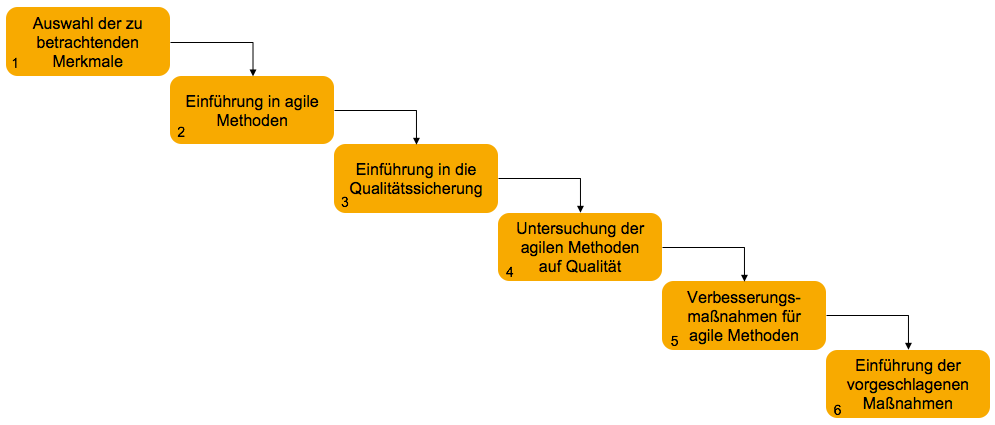
\includegraphics[width=\textwidth]{Abbildungen/ablauf}
                    \caption{Vorgehensweise dieser Arbeit}
                    \label{abb:ablauf}
                \end{center}
        \end{figure}

        Um die Qualität einer Software zu erfassen, müssen Kriterien gegeben sein, anhand derer sie bewertet wird. In Schritt 1 der Abbildung wird zunächst die Qualität definiert und anschließend werden Merkmale definiert, die für qualitative Software betrachtet werden müssen. Aus diesen Merkmalen werden die für die Bausparkasse Relevantesten ausgewählt und im weiteren Rahmen dieser Arbeit betrachtet.

        In \autoref{cha:vorgehensmodelle} werden Softwareprojekte definiert und als Beispiel für eine klassische Herangehensweise das Wasserfallmodell vorgestellt. Im Anschluss wird der Fokus auf agile Verfahren gelegt, wobei zunächst die Prinzipien des agilen Manifests und anschließend verschiedene agile Softwareentwicklungsprozesse erläutert werden. Die agilen Prozesse bilden die Grundlage der Analyse dieser Arbeit und sollen optimiert werden.

        Im folgenden Kapitel wird eine Einführung in die Qualitätssicherung gegeben. Hier wird zwischen verschiedenen qualitätssichernden Maßnahmen differenziert und es werden ausgewählte Methoden zur Sicherstellung und Verbesserung der Qualität im Softwareentstehungsprozess aufgezeigt. Teile dieser Methoden sollen auf die agilen Entwicklungsprozesse angewandt werden, um die Qualität in agilen Prozessen zu verbessern und eine umfassende Sicherung der Qualität zu gewährleisten.

        In \autoref{cha:prozessentwicklung} (Schritt 4) werden die agilen Entwicklungsverfahren beleuchtet und Stärken und Schwächen aufgedeckt. Auf Basis der qualitätssichernden Maßnahmen aus \autoref{cha:einfuehrungQS} werden die agilen Entwicklungsverfahren in Schritt 5 ergänzt. Dies dient als Orientierungshilfe zur qualitätssichernden Erweiterung von agilen Prozessen.

        Damit dieser Prozess kontrolliert und ordnungsgemäß durchgeführt wird, werden erneut Qualitätssicherungsmodelle aus \autoref{sec:qsmethoden} angewandt. Der Soll-Prozess wird mit jeder Iteration kontrolliert und verbessert, damit das Ergebnis des Projekts möglichst alle Anforderungen erfüllt. Die Vorgehensweise hierfür wird skizziert.

        Zum Abschluss werden die Arbeitsergebnisse kritisch bewertet und Möglichkeiten aufgezeigt, diese in der Praxis anzuwenden. 
    %%In den Grundlagen wird das Ziel aller Rahmenwerke, die serviceorientierte Architektur, vorgestellt. Im Anschluss werden alle Rahmenwerke vorgestellt und wichtige Begriffe definiert. Im Hauptteil werden die Kernpunkte des BIAN beleuchtet und mit den äquivalenten Schritten der anderen Rahmenwerke verknüpft. Dabei werden die wesentlichen Unterschiede herausgestellt und bewertet. Im Anschluss werden Verbesserungsvorschläge für die ASAP Methodik gegeben und ein kritisches Fazit gezogen.

\chapter{Grundlagen}

 %   Faktoren zur Messung von Softwarequalität anhand der ISO 9126 vorgestellt und deren Relevanz für diese Bachelorarbeit werden bewertet.

 %   Im Kapitel Grundlagen wird das Konzept der agilen Softwareprogrammierung aufgezeigt und im Nachgang einige ausgewählte Methoden vorgestellt. Aus diesen wird eine Methode ausgewählt, die im Rahmen dieser Bachelorarbeit als Beispiel genutzt wird. Die Vorgehensweise zur Qualitätssicherung ist gleich.

    Im folgenden Kapitel wird der Begriff der Qualität definiert, um anschließend die Qualitätsmerkmale von Software festzulegen. Diese werden auf Grundlage der allgemein gehaltenen ISO 9126-1 definiert, die die Grundlage zu vielen spezifischeren Qualitätsmodellen darstellt. Von diesen Qualitätsfaktoren wird eine bestimmte Menge ausgewählt, die für die Qualitätsprozesse im Rahmen dieser Bachelorarbeit als Kriterien herangezogen werden.

    Im Anschluss daran wird das Konzept der agilen Softwareentwicklung vorgestellt. Neben der Entstehungsgeschichte und den Vor- bzw. Nachteilen der agilen Entwicklung werden verschiedene Vorgehensweisen vorgestellt.

    Daraufhin wird mit den Qualitätssicherungssystemen ebenso verfahren.

    Die Methodiken werden im darauf folgenden Kapitel verglichen und bewertet.

%----------------------------------
%
% Definition von Qualität
%
%----------------------------------
    \section{Definition von Qualität}

        Da der Begriff Qualität im Alltag häufig und in verschiedenen Situationen verwendet wird, soll hier eine Grunddefinition des Qualitätsbegriffs gegeben werden, der im Rahmen der vorliegenden Bachelorarbeit verwendet wird.

        Es kann gesagt werden, \enquote{dass Qualität
            \begin{itemize}
                \item eine Menge von Eigenschaften repräsentiert, die einem Produkt oder Verfahren immanent oder beigegeben ist.
                \item einer der Maßstäbe ist, mit dem der Kunde seine Kaufentscheidung herbeiführt.
                \item ein Faktor ist, der in intensiver Wechselwirkung mit der Wettbewerbssituation und Leistungsfähigkeit eines Anbieters steht.
            \end{itemize}
            \footnote{Pfeifer, 1990.}}

        Dies verfeinert die Definition der ISO 9000: \enquote{Qualität ist der Grad, in dem ein Satz inhärenter Merkmale Forderungen erfüllt\footnote{ISO 90003, 2008, S..}.} Für Qualität bedeutet das, dass einem Werksstück, Prozess oder auch einer Software messbare und nicht messbare Eigenschaften inne wohnen. Bei Software unterscheidet man beispielsweise zwischen messbaren, funktionalen Anforderungen und nicht messbaren, nicht funktionalen Anforderungen. Ein Beispiel für eine funktionale Anforderung ist die Antwortzeit eines Programms, während ein \enquote{gutes} User Interface einer nicht funktionalen Anforderung entspricht. Inhärent sind Merkmale, die sich nach Auslieferung nur sehr schwer oder gar nicht verändern lassen, während der Preis als Beispiel für ein nicht-inhärentes Merkmal sehr frei zu gestalten ist.

        Ein wichtiges Merkmal der vorangehenden Definition ist allerdings die Qualität als Merkmal der Kundenbeeinflussung. Dabei stellt sie sich als Merkmal dar, dass für oder auch gegen die Kaufentscheidung eines bestimmten Produktes spricht. Als Hersteller ist somit eine Sicherung der Qualität unumgänglich um nachhaltig am Markt zu agieren.

%----------------------------------
%
% Qualitätsmerkmale von Software
%
%----------------------------------
    \section{Qualitätsmerkmale von Software}

        Nachdem Qualität als wichtiges Merkmal zum Bilden und Fortbestehen eines Unternehmens identifiziert wurde gilt es nun die Qualität messbar zu machen.

        Die ISO 9126 stellt hierzu sechs Charakteristiken bereit, auf deren Grundlage die Qualität von Software bewertet werden kann. Diese sind in 27 Unterdimensionen unterteilt auf die in den einzelnen Unterpunkten eingegangen wird.
        %Außerdem stellt die ISO 9126 Maßstäbe bereit, um die Unterkategorien zu messen und anhand derer die Erfüllung der Charakteristiken zu bewerten.

        Betrachtet werden nachfolgend die Oberpunkte mit einer Definition nach ISO 9126 und einer Erläuterung. Die ISO Definitionen der Unterkategorien befinden sich im Glossar. Im Anschluss werden drei Merkmale gewählt, die im Rahmen dieser Arbeit betrachtet werden.

    \subsection{Vorstellung der Qualitätsmerkmale}

        Die folgenden Zitate und Absätze orientieren sich vollständig an der ISO 9126-1 Richtlinie.

        \subsubsection{Funktionalität}

            \begin{quote}
              The capability of the software product to provide functions which meet stated and implied needs when the software is used under specified conditions\footnote{ISO 9126-1, 2000, S.7.}.
            \end{quote}

            Die Charakteristik Funktionalität gibt die Fähigkeiten der Software an. Beispielsweise ist eine Funktionalität einer Buchhaltungssoftware die Berechnung einer Gewinn- und Verlustrechnung. Im Gegensatz zu den folgenden Charakteristiken gibt diese an, was die Software tut, statt zu sagen auf welche Weise sie etwas tut.

            Darunter fallen die Abdeckung der gestellten Anforderungen an Funktionalität und Genauigkeit, sowie Sicherheitsaspekte. Im Falle der SAP hat ein Softwareprodukt beispielsweise die Funktion der Geschäftspartnerverwaltung und sollte somit alle fachlich an sie gestellten Anforderungen bedienen. Außerdem sollte bei einer identischen Eingabe stets ein identisches, erwartetes Resultat entstehen. Durch den Scope der zu Beginn eines Projektes erstellt wird ist diese Charakteristik meist schon zu Beginn eines Projekts genau spezifiziert.

            Kunden kaufen Software in der Annahme, dass diese einen Mehrwert für diesen darstellt. Das bedeutet, dass die Software die Arbeit des Kunden erleichtert oder die Qualität seiner Arbeit erhöht. Damit ein Mehrwert geschaffen werden kann müssen die versprochenen Funktionen abgedeckt sein. Eine Software zur Verwaltung von Geschäftspartnern würde keinen Mehrwert liefern, wenn es nicht möglich wäre neue Geschäftspartner anzulegen.


        \subsubsection{Verlässlichkeit}

            \begin{quote}
              The capability of the software product to maintain a specified level of performance when used under specified conditions\footnote{ISO 9126-1, 2000, S.8.}.
            \end{quote}

            Die Charakteristik Verlässlichkeit gibt die Fähigkeit einer Software an unter den festgelegten Rahmenbedingungen immer in einem vorher festgelegten Rahmen zu reagieren. In alten Definitionen bezog sich die Verlässlichkeit darauf eine bestimmte, benötigte Funktion auszuführen.

            Das Ziel ist eine Software, die zu jederzeit in dem erwarteten Umfang reagiert und falsche Eingaben, falsche Benutzungsweisen und ungültige Datensätze verkraftet oder verhindert. Software ist genau dann verlässlich, wenn keine Fehler durch Defekte in der Software auftreten, keine Angriffe, bewusst oder unbewusst, von außen oder innen möglich sind und sämtliche Daten auch nach einem Systemabsturz wieder herstellbar sind.

            Unternehmen der Finanzindustrie besitzen häufig Softwarelandschaften, die in den 1970er Jahren aufgebaut werden und seitdem im Stand gehalten und erweitert werden.\footnote{Vgl. TOGAF/Bian, 2013, S.10.} Die auf Mainframes aufgebauten Architekturen sind sehr teuer in Wartung und Entstandhaltung, aber gewährleisten eine hohe Erreichbarkeit von bis zu 99.999\%. Dies bedeutet, dass ein Mainframe nur circa 5,26 Minuten pro Jahr nicht zu erreichen ist. IBM gibt für ihre Mainframes zudem eine durchschnittliche Zeit zwischen Fehlern von 20 bis 30 Jahren an. Außerdem werden Operationen häufig mehrfach gleichzeitig durchgeführt und die Ergebnisse verglichen. Somit sind fehlerhafte Berechnungen nahezu ausgeschlossen.\footnote{Symonds, 2013, S.12.} Unternehmen der Finanzindustrie stellen somit hohe Anforderungen an ihre IT Systeme und die zuverlässige Ausführung von Prozessen ist bei der Verarbeitung von Zahlungsströmen u.ä. unverzichtbar.

        \subsubsection{Benutzerfreundlichkeit}

            \begin{quote}
              The capability of the software product to be understood, learned, used and attractive to the user, when used under specified conditions\footnote{ISO 9126-1, 2000, S.9.}.
            \end{quote}

            Benutzbarkeit sagt aus, dass ein fachlich versierter Anwender intuitiv die Funktion des Programms erkennt und es verwenden kann. Dabei soll der Anwender nach Möglichkeit ein gutes Gefühl haben und die Software als schön bezeichnen.

            Das Ziel der SAP ist es durch eine intuitive Menüführung beim Endbenutzer einen Produktivitätszuwachs zu erreichen, indem dieser schnell und sicher durch die Oberfläche navigieren kann. Durch leicht zu verstehende Oberflächen soll zudem die zur Einarbeitung benötigte Zeit reduziert werden. Somit wird im Idealfall der Schulungsbedarf des Kunden reduziert.

            Aus dem Privatleben sind geschäftliche Anwender inzwischen einfache, intuitive Oberflächen gewöhnt und tragen diese als Anforderung ins Unternehmen. Außerdem werden mehr mobile Geräte in Unternehmen verwendet. Um alle Daten, zu jeder Zeit und an jedem Ort zur Verfügung zu haben werden die Daten häufig in der Cloud bereitgestellt und über webbasierte Applikationen angezeigt. SAP verfolgt mit dem Paradigma Fiori die Strategie, dass sich die Oberflächen zwischen mobilen Geräten und Computern nicht unterscheiden und keine Daten auf dem Gerät liegen. Durch einheitliche Oberflächen soll die Produktivität der Nutzer erhöht werden und die Einarbeitungszeit reduziert werden.

        \subsubsection{Effizienz}

            \begin{quote}
              The capability of the software product to provide appropriate performance, relative to the amount of resources used, under stated conditions.
            \end{quote}

            Der Faktor Effizienz drückt das Verhältnis zwischen der Performance der Software und den dafür verbrauchten Ressourcen aus. Die Effizienz steigt, wenn die Performance bei gleichbleibendem Ressourcenverbrauch steigt oder wenn bei gleichbleibender Performance der Ressourcenverbrauch sinkt und umgekehrt.

            Um selbst bei umfangreichen Datenabfragen und Berechnungen eine geringe Antwortzeit zu gewährleisten verfolgt SAP den Trend der In-Memory Datenhaltung. SAP verwendet hierzu die SAP High Performance Analytical Appliance (HANA). Trotz der gestiegenen Ressourcennutzung ist der Performance Gewinn größer um deren Verwendung zu rechtfertigen. Gerade im Umgang mit Massendaten, die im Finanzbereich anfallen ist eine effiziente Datenhaltung und Verarbeitung sehr empfehlenswert.

        \subsubsection{Wartbarkeit}

            \begin{quote}
              The capability of the software product to be modified. Modifications may include corrections, improvements or adaptation of the software to changes in environment, and in requirements and functional specification.
            \end{quote}

            Die Wartbarkeit einer Software wird anhand der Möglichkeit bewertet Korrekturen, Verbesserungen und neue Funktionen einzuspielen. Außerdem sollte die Software an neue Anforderungen, wie neue Prozesse oder neue Umsysteme anpassbar sein.

            Eine stetige Zunahme an regulatorischen Anforderungen in einem dynamischen Marktumfeld erfordern flexible und modulare Systeme. Da kein allumfassendes Softwareprodukt pro Branche bereit gestellt werden kann müssen die Systeme in ihre Umgebung, insbesonde historisch gewachsene, bestehende Systeme, eingegliedert werden.

        \subsubsection{Portierbarkeit}

            \begin{quote}
              The capability of the software product to be transferred from one environment to another.
            \end{quote}

            Die Portierbarkeit der Software ist besonders hoch, wenn sie so universell programmiert ist, dass sie ohne oder mit minimalem Aufwand auf verschiedenen Infrastruktur und Software Plattformen verwendet werden kann. Für SAP als Anbieter von Standardsoftware ist dies einer der Hauptfaktoren zur Entwicklung von Software, da dies die Grundlage zur Wiederverwendung von entwickelten Softwarebausteinen bildet.

        \subsection{Auswahl und Bewertung der Qualitätsmerkmale}

            Funktionalität bewertet den Funktionsumfang der Software. Wenn die Software nicht alle wichtigen Anforderungen des Kunden erfüllt ist die Investition in diese Software nicht gewinnbringend und er wird sie nicht tätigen. Daher wird die Funktionalität als erstes Bewertungskriterium in dieser Arbeit herangezogen.

            Die korrekte und vollständige Ausführung von Operationen auf der Software ist für Unternehmen der Finanzdienstleistungsindustrie sehr wichtig, da Kunden einen hohen Standard gewohnt sind und Fehler sehr kostspielig sein können. Es ist daher essentiell, dass die Software verlässlich arbeitet, korrekte Ausgaben erzeugt und die Daten sicher hält. Verlässlichkeit wird daher auch als Bewertungskriterium in dieser Arbeit herangezogen.

            Benutzerfreundlichkeit wird hauptsächlich durch die Anwendungsoberfläche bestimmt. Die Implementierung von Software ermöglicht es zudem die Anwendungsoberfläche unabhängig von der Datenhaltung und der Datenverarbeitung zu erstellen in einer so genannten 3-Schichten-Architektur. Da die Endanwender häufig nicht die Käufer einer Software sind und für SAP durch reduzierten Schulungsbedarf kein unmittelbarer Mehrwert entsteht ist eine intuitive und selbsterklärende Oberfläche nicht kritisch für den Verkauf von Software und einer Zufriedenstellung des Kunden. Die Benutzerfreundlichkeit der Software wird im Rahmen dieser Arbeit außen vor gelassen.

            Bausparverträge und Baufinanzierungen sind meist langfristig orientierte Verträge und werden nach einer umfassenden Beratung und im idealfall auch nach einem Vergleich von Angeboten angelegt und unterschrieben. Das bedeutet, dass innerhalb dieses Geschäftszweigs keine Echtzeitdaten benötigt werden, sondern eine zeitnahe Beantwortung von Anfragen ausreicht. Für die Effizienz bedeutet dies, dass mit einem vertretbaren Aufwand vertretbare Resultate erzeugt werden sollen, ohne das technische Grenzen ausgereizt werden müssen. Effizienz ist daher kein Teil der in dieser Arbeit betrachteten Kriterien.

            Die Finanzindustrie untersteht einem stetigen, disruptiven Wandel, der durch neue regulatorische Anforderungen und neue Konkurrenzen, sogenannte Fin-Techts, verursacht wird. Die neuen Marktteilnehmer bauen ihre IT ohne störende Altlasten auf und können so dynamisch auf das Marktumfeld reagieren. Um auch die eigene Software zukunftsfähig zu machen und selbst konkurrenzfähig zu bleiben muss eine Unternehmensplattform anpassbar und flexibel sein. Eine leicht zu wartende Lösung reduziert die Betriebskosten und bildet die Grundlage zur zukunftsfähigen IT. Wartbarkeit ist daher ein wichtiges Kriterium und bidet somit das letzte Kriterium, dass im Rahmen dieser Arbeit verwendet wird.

            Da SAP als reiner Softwarehersteller keine Hardware verkauft muss SAP Software auf verschiedenen Platformen und Betriebssystemen anwendbar sein. Da SAP Instanzen in eigenen Laufzeitumgebungen auf dem Betriebssystem laufen ist die Kompabilität der Software mit verschiedenen Betriebssystemen keine Aufgabe der Entwickler für Geschäftsanwendungen. Diese Charakteristik ist daher ebenso zu vernachlässigen.

            Im Folgenden wird daher für den Entwicklungsprozess eine funktionale, verlässliche und wartbare Software als Ziel festgesetzt.

%----------------------------------
%
% Agile Methoden
%
%----------------------------------
    \section{Agile Methoden}

        \begin{quote}
          Achieving a product which satisfies the user's needs normally requires an iterative approach to software development with continual feedback from a user perspective.\footnote{ISO 9126-1, 2000, S.4.}
        \end{quote}

        Agile Methoden wurden mit dem Ziel entwickelt den Endbenutzer früher in die Softwareentwicklung einzubeziehen, um ein Produkt zu entwerfen, dass tatsächlich benötigt wird. Hierzu werden möglichst schnell und möglichst viele einzelne, aber lauffähige Code-Fragmente entwickelt, die dem Kunden vorgeführt werden um diesen ein Gefühl für die Software zu geben. Das frühe Feedback des Kunden ermöglicht es schon früh während des Entwicklungsprojekts Anpassungen vorzunehmen um die realen Bedürfnisse zu erfüllen.

        Hierzu wurden Prinzipien entwickelt, die einfach und granular die Idee der agilen Entwicklung herunterbrechen. Diese wurden im agilen Manifest festgehalten und verbreitet. Hierbei ist zu beachten, dass jeweils nicht nur der erste Teil der Prinzipien beachtet werden soll, sondern dieser eine höhere Gewichtung zukommt.\footnote{Vgl. Agile Manifesto, 2015.}

        \subsection{Prinzipien der agilen Entwicklung}

            \subsubsection{Individuals and interactions over processes and tools}

                Software Entwicklung wurde vor den agilen Entwicklungsmethoden sehr weit standardisiert und geplant\footnote{Vgl. Schneider, 2007, S..}. Hierdurch waren die Entwickler häufig sehr unflexibel und konnten nicht auf Wünsche oder Anpassungsvorschläge reagieren, sobald diese den Zeitplan verletzt hätten.

                Um dieser Entwicklung entgegenzuwirken stellt das agile Manifest die Interaktion mit dem Kunden und unter den Entwicklern an erste Stelle, anstatt das diese von Prozessen regiert werden.

                Ein reger Austausch soll gefördert und auf die Bedürfnisse der einzelnen Personen soll eingegangen werden.

            \subsubsection{Working software over comprehensive documentation}

                Durch viel bürokratischen Aufwand und eine umfangreiche Planung von Software wird zu Beginn des Projektes sehr viel Aufwand investiert ohne einen konkreten Mehrwert gegenüber stehen zu haben. Durch die dynamische Grundhaltung bei der agilen Entwicklung wird zu Beginn sehr wenig Zeit in die Planung investiert, die Entwicklung kann direkt gestartet werden und schon nach kurzer Zeit gibt es lauffähige Programmbestandteile.

                Dieses Prinzip drückt aus, dass am Ende eines Projekts eine lauffähige Software, die die Ansprüche des Kunden erfüllt einer umfangreichen Dokumentation mit unvollständiger Software zu bevorzugen ist.

            \subsubsection{Customer collaboration over contract negotiation}

                SAP hat als Hersteller von Standardsoftware zur Unternehmenssteuerung das Ziel Software zu entwickeln und diese zu verkaufen. Der Verkauf von Software wird erheblich erleichtert, wenn diese ein Bedürfnis des Kunden erfüllt und bei diesem die tägliche Arbeit erheblich vereinfacht.

                Um die Anforderungen des Kunden zu verstehen und bei der Entwicklung der Software zu berücksichtigen sollte dieser schon früh einbezogen werden. Die agilen Methoden sollen dabei auf die Wünsche des Kunden reagieren, statt jede Abweichung eines aufgestellten Plans mit umfangreichem bürokratischen Aufwand zu verhandeln.

            \subsubsection{Responding to change over following a plan}

                Insbesondere bei längeren Projekten ist es meist absurd anzunehmen, dass man die Anforderungen des Unternehmens in ferner Zukunft kennt. Bei Unternehmen der Finanzindustrie werden häufig neue regulatorische Anforderungen veröffentlicht oder das Marktumfeld verändert sich. Um auf diese Änderungen auch während der Projektlaufzeit eingehen zu können und keine zum Release veraltete Software einzusetzen sollte im Projekt auf Veränderungen eingegangen werden.

        \subsection{Ausgewählte Methoden der agilen Entwicklung}

            Im Folgenden werden konkrete herangehensweisen zur agilen Entwicklung vorgestellt. Diese sind genau wie die Prinzipien des agilen Manifests sehr allgemein und locker gehalten um den Entwicklern hinreichend Freiraum zu geben um Ideen ausleben zu können. Dies entspricht der Idee der agilen Entwicklung.

            \subsubsection{Lean Software Development}

                Die Grundlage des Lean Software Developments bildet der Produktentwicklungsprozess von Toyota. Im Anschluss an den zweiten Weltkrieg wurde dort die Automobilproduktion aufgebaut und da in Japan weder der Platz noch die Ressourcen vorhanden waren um die ineffiziente amerikanische Automobilproduktion zu immitieren wurden neue Prinzipien in die Entwicklung integriert, die die Lagerhaltung, Massenfertigung und Produktentwicklung betreffen.\footnote{Vgl. Dombrowski, 2015, S.7.} Der Entwicklungsprozess baut auf sieben Prinzipien auf, die zusammen mit agilen Methoden auch auf die Softwareentwicklung angewendet werden können.

                Die bisherige Annahme im Produktentwicklungsprozess, unabhängig von Software, Autos o.ä., war, dass ein Fehler, der während der Planung eliminiert wird um den Faktor 1000 günstiger ist als ein Fehler, der beim Kunden entdeckt wird. Dies leitet sich aus der so genannten Zehnerregel der Fehlerkosten ab:

                \begin{figure}[!htbp]
                        \begin{center}
                        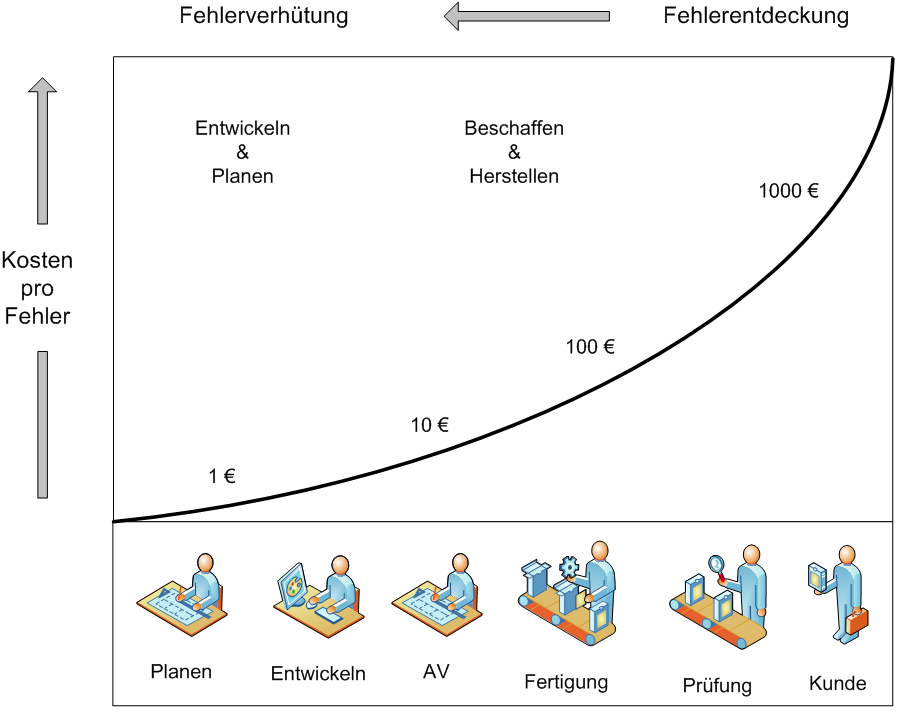
\includegraphics[width=11cm]{Abbildungen/zehnerregel}
                        \caption{Zehnerregel der Fehlerkosten\protect\footnotemark}
                        \label{abb:zehnerregel}
                        \end{center}
                \end{figure}

                \footnotetext{http://www.sixsigmablackbelt.de/fehlerkosten-10er-regel-zehnerregel-rule-of-ten/}

                Im Rahmen von Lean Development halten sich die praktizierenden Unternehmen während des Designprozesses jedoch möglichst viele Optionen offen, um während des Produktionsprozesses Entscheidungen auf einer optimalen Faktenbasis zu treffen und nicht durch plausible Annahmen.\footnote{Vgl. Poppendieck, 2003, S.5.} Solche Design- und Funktionsentscheidungen sehr spät im Prozess zu treffen wird beispielsweise in Scrum praktiziert, indem erst zu Beginn jedes Sprints die Anforderung des Kunden festgelegt wird und nicht in einem umfangreichen Scopedokument zu Beginn des gesamten Projektes.

                Die Prinzipien des Lean Developments lassen sich als agilen Prozess anwenden oder auf agile Prozesse ummünzen. Folgende Prinzipein wurden als Kern des Lean Development identifiziert\footnote{Poppendieck, 2003, S. 13.}:

                \begin{itemize}
                  \item Eliminate waste
                  \item Amplify learning
                  \item Decide as late as possible
                  \item Deliver as fast as possible
                  \item Empower the team
                  \item Build integrity in
                  \item See the whole
                \end{itemize}

                Im folgenden wird eine kurze Einführung der Unterpunkte gegeben mit einer Erläuterung, wie sie als agiler Prozess aufzusetzen sind.

                \enquote{Waste is anything that does not add value to a product, value as perceived by the customer.}\footnote{Poppendieck, 2003, S.13.} Dies umfasst bezogen auf die Softwareentwicklung nicht nur sämtliche Applikationen, die nicht benötigt werden, sondern auch ungenutzte Funktionen und das potenzial zu möglichen, zukünftigen Erweiterungen im Code. Das Ziel sollte es sein den Code so klein wie möglich zu halten um die unmittelbaren Bedürfnisse des Kunden zu befriedigen. Das bedeutet, dass in jeder Iteration des Entwicklungsprozesses nur die Funktion entwickelt wird, die der Anwender braucht und die am höchsten priorisiert ist. Rein statistisch werden etwa 50\% aller Funktionen einer Software selten oder nie genutzt\footnote{Ebert, 2007} Wenn dieser Überschuss eliminiert wird werden die Programme schlanker, einfacher und günstiger in der Wartung, ohne das der Anwender auf wichtige Funktionen verzichten muss.

                Die Entwicklung eines Produktes ist im Gegensatz zur Herstellung eines Produktes kein linearer Prozess, der vorher skizziert und abgearbeitet werden kann. Obwohl Variation in der Produktion reduziert beziehungsweise eliminiert werden soll ist sie im Entstehungsprozess eines Produkts durchaus wünschenswert, um die bestmögliche Lösung zu finden.\footnote{Vgl. Ballard, 2000, S. 2f.} Um möglichst viele Optionen zu betrachten und sich mit fortgeschrittenem Kenntnisstand für eine zu entscheiden hat Toyota das so genannte \emph{Set-Based Concurrent Engineering} entwickelt, bei dem mehrere Prototypen in die Entwicklung mitgeführt werden, statt zu Entwicklungsbeginn einen Designstop einzulegen. Diese Protoypen werden mit dem jeweils aktuellen Kenntnisstand weiterentwickelt und eine Entscheidung zu Gunsten einer Variante fällt so spät wie möglich. Zur Entwicklung dieser Methoden wird ein Prozess von drei Oberpunkten vorgesehen, die die Menge von Möglichkeiten filtern:

                \begin{itemize}
                  \item Map the design space
                  \item Integrate by intersection
                  \item Establish feasibility before commitment\footnote{Sobek, 2000, S.73.}
                \end{itemize}

                Zunächst wird daher der Rahmen festgelegt, in dem entwickelt werden darf. Dies betrifft übertragen auf die Softwareentwicklung Programmiersprachen und Systeme. Im Anschluss werden Konzepte in diesem Rahmen übereinandergelegt und die Variation auf das nötigste reduziert. Abschließend werden alle verbliebenen Vorgehensweisen auf Machbarkeit geprüft und auf Basis dieses Ergebnisses eine Entscheidung getroffen. Die Reduzierung der Grenzen bis zur Entscheidung für eine Vorgehensweise lernen die Entwickler aus dem Entwicklungsprozess und die Möglichkeit, die den größten Nutzen bietet wird umgesetzt.
                Dies ist auch der Grund dafür, dass eine möglichst späte Entscheidung angestrebt wird.

                Die Vorgabe so schnell wie möglich Ergebnisse zu liefern bedeutet nicht, dass ein unfertiges oder unreifes Produkt ausgeliefert werden soll, sondern das lauffähige Versionen entstehen, auf deren Grundlage die Entwicklung voranschreiten kann. Somit kann ein Kunde herausfinden was er benötigt und die Richtung des Projektes besser gesteuert werden. Dies führt zu kurzen Iterationen, die lauffähige Ergebnisse liefern.

                Der reine Einsatz von Methoden führt häufig nicht zu den gewünschten Ergebnissen. Es geht ebenfalls darum die Mitarbeiter in den Prozess der Produktentstehung einzubinden und alle Ideen und Kompetenzen zu nutzen. Bisherige Softwareentwicklungsprozesse zielen darauf ab zu Beginn der Entwicklung Entscheidungen von einer Hand voll Personen zu treffen, die die tatsächliche Implementierung meist nicht persönlich umsetzen. In einem Lean Development Umfeld sollen die Entscheidungen von den umsetzenden Personen getroffen werden und die oberen Hierarchien durch Reports, Grafiken und regelmäßige Meetings lediglich informiert werden. Dies beschleunigt Iterationen und ermöglicht mehr Tests und Versuche, die zu besseren Ergebnissen führen.\footnote{Vgl. Poppendieck, 2003, S.14}

                Die Integrität einer Software wird daran gemessen, wie zufrieden jemand ist, der mit dieser Software arbeitet, unabhängig davon ob eben dieser Anwender oder Entwickler ist. Hierbei beruft sich Poppendieck auf die Qualitätskriterien von Software der ISO 9126-1, die oben vorgestellt wurden. Sie sagt, dass dies nicht durch Prozesse und Messungen umsetzbar sei, sondern durch weise Führung, fachliche Expertise, effiziente Kommunikation und gesunde Disziplin.\footnote{Vgl. Poppendieck, 2003, S.14.} Der Weg zur Integrität einer Software basiert daher auch auf einigen Prinzipien des agilen Manifests.

                Zuletzt soll das Gesamtziel des Projektes nicht aus den Augen verloren werden. Die absolute Optimierung eines Teilbereichs zu Lasten des Gesamtprojekts sollte zwingend vermieden werden.

                Zusammenfassend ist Lean Software Development eine Menge von Prinzipien, die aus der Entwicklung von Autos abgeleitet wurde und zu Beginn eines Projektes als konkrete Pläne umgesetzt werden sollen. Wie die im Folgenden vorgestellten agilen Programme weißt es auf typische Fehler hin und gibt Ratschläge, wie sie vermieden werden können, ohne die Freiheit des Teams einzuschränken.

            \subsubsection{Extreme Programming}

                \begin{quote}
                  XP is a style of software development focusing on excellent application of programming techniques, clear communication, and teamwork which allows us to accomplish things we previously could not even imagine.\footnote{Andres, 2005, S..}
                \end{quote}

                \enquote{Extreme Programming ist eine leichtgewichtige Softwareentwicktlungs-Methode, mit einem Wertesystem sowie einer Sammlung von Grundprinzipien und Entwicklungspraktiken\footnote{Rumpe, 2001, S..}.}
                Extreme Programming räumt mit einigen Konventionen der Softwareentwicklung auf, indem es die bisher bestehenden Prozesse bewusst kritisiert und eigene Werte und Modelle präsentiert, die die Softwareentwicklung vereinfachen.

                Extreme Programming orientiert sich dennoch an einem groben Prozess zur Entwicklung von Software. Zunächst wird eine User Story entworfen, das heißt ein Anwender beschreibt was er tun muss und an welchen Stellen er dabei unterstützt werden müsste. Zur Erläuterung des Prozesses wird nachfolgend das Anlegen eines Vertrags in einer Filiale aus Sicht eines Angestellten betrachtet.

                Der Anwender möchte die Daten des Kunden in die Softwareoberfläche eintragen und anschließend einen Vertrag mit den Konditionen für diesen Kunden ausdrucken. Die Daten sollen zudem in der Datenbank der Bausparkasse hinterlegt werden. Daraus ergibt sich eine neue Aufgabe für die Softwareentwickler.

                Extreme Programming sieht vor, dass für jede zu entwickelnde Komponente zunächst ein Test geschrieben wird. Die Tests bilden das pendant zur klassischen Spezifikation und werden nach jeder Änderung der Software überprüft um so eine ständige Lauffähigkeit des Moduls zu gewährleisten. Ein Test würde beispielsweise prüfen, wie mit unvollständigen Angaben umgegangen wird und wenn kein Drucker erreichbar wäre. Bei der Erstellung der Test-Fälle sollten alle gewöhnlichen Eingaben, ungültige Eingaben und Randwerte, wie zum Beispiel unendlich große bzw. unendlich kleine Bausparsummen geprüft werden.\footnote{ANGABE SUCHEN}

                Auf Grundlage der entworfenen Tests startet die Entwicklung, die die Ansprüche des Anwenders, die im Test formalisiert wurden, erfüllen soll. Im Gegensatz zur klassischen Entwicklung von Software, bei der jeder Entwickler für einen Baustein das Programms zuständig ist und diesen in Einzelarbeit vorantreibt wird im Extreme Programming Pairprogramming empfohlen. Außerdem sollen alle Entwickler jederzeit den gesamten Code kennen und dürfen an jeder Stelle etwas verändern, sobald sie Fehler entdecken. Das Ziel ist es die Abhängigkeit von einzelnen Entwicklern zu reduzieren und schon während der Entwicklung eine ständige Kontrolle durch den Partner zu haben. Studien haben außerdem nachgewiesen, dass zwei Entwickler die Entwicklungszeit reduzieren und weniger Fehler produzieren\footnote{ANGABE SUCHEN}.

                \begin{figure}[!htbp]
                    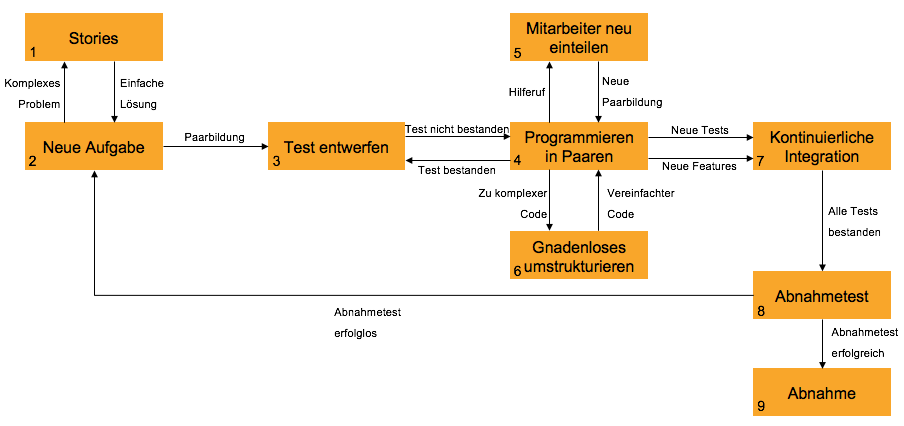
\includegraphics[width=15cm]{Abbildungen/XP_vorgehensmodell}
                    \caption{Vorgehensmodell des Extreme Programming\protect\footnotemark}
                    \label{abb:xpmodel}
                \end{figure}

                \footnotetext{https://www.st.cs.uni-saarland.de/edu/lehrer/xp.pdf, 2016.}

                Extreme Programming hat darüber hinausgehend noch zwei Prinzipien, die bei der klassischen Softwareentwicklung in dieser Form nicht angewendet werden. Zunächst wird immer nur ein aktuelles Problem gelöst und es werden keine Pläne für zukünftige Integrationen und Erweiterungen im Code umgesetzt. Der Code soll so einfach wie möglich gehalten werden und die Voraussetzung ist, dass ein einfacher Code später besser anzupassen ist, als komplizierten Code mit einer Schnittstelle zu haben, die eventuell nie gebraucht wird.

                Das zweite Prinzip ist der selbstdokumentierende Code. Über sprechende Methodennamen und Kommentare soll jeder Entwickler zu jeder Zeit verstehen, was sich der Autor des Codes gedacht hat. Dieser sprechende Code soll die Dokumentation der Software obsolet machen. Dies geschieht aus dem Grund, dass Dokumentationen häufig nicht aktuell sind oder nicht mit dem gleichen Eifer wie der Code entwickelt wurden und somit fachlich falsch sind. Diese Ziele werden erreicht, indem sehr viele Kommentare verwendet werden und das bisher entwickelte \emph{Refactored} wird. Das bedeutet, dass Codebruchstücke, wie beispielsweise eine Tabellenabfrage in eine Methode ausgegliedert werden und stattdessen die Methode im Hauptprogramm aufgerufen wird. Diese ständigen Restrukturierungen vereinfachen das bisher entwickelte und lassen den Umfang des Programms nicht ausufern.

                Natürlich stößt aber auch das Extreme Programming in Projekten an Grenzen. Die Pairprogramming Methodiken setzen voraus, dass die Entwickler auf engem Raum zusammen arbeiten und nicht allzu weit verstreut sind. Außerdem muss für die ständige Abstimmung und Kommunikation das Team sehr klein gehalten werden, meist werden 9-12 Personen empfohlen.

                Extreme Programming stellt konkrete Anforderungen an das Team und lässt in der Umsetzung die wenigsten Freiheiten der agilen Methoden. Es ist, wie der Name impliziert, eine sehr extreme Herangehensweise, die Tests, Entwicklung und Flexibilität maximiert. Häufig können jedoch vereinzelte Methoden des Extreme Programming in anderen agilen Verfahren verwendet werden um ein Teil von methodischer Flexibilität zu erhalten.

            \subsubsection{Scrum}

                  Scrum ist ein \enquote{Ein Rahmenwerk, innerhalb dessen Menschen komplexe adaptive Aufgabenstellungen angehen können, und durch das sie in die Lage versetzt werden, produktiv und kreativ Produkte mit dem höchstmöglichen Wert auszuliefern.} Es ist
                  \begin{itemize}
                      \item Leichtgewichtig
                      \item Einfach zu verstehen
                      \item Schwierig zu meistern.\footnote{Scrum Guide, 2013, S..}
                  \end{itemize}

                  Im Gegensatz zum Extreme Programming ist Scrum ein Rahmenwerk statt einer Methode, dass neben konkreten Managementvorgaben sehr viel Gestaltungsfreiraum bietet. Scrum setzt auf einen iterativen, inkrementellen Ansatz, was bedeutet, dass kurze Phasen der Entwicklung ständig wiederholt werden und das Endprodukt Stück für Stück aufgebaut wird. Mit jeder abgeschlossenen Phase wird die Software um einen weiteren Baustein ergänzt.

                  Für nach Scrum organisierte Teams wird eine Personenanzahl von 5-9 Entwicklern zuzüglich Scrum Master und Product Owner empfohlen. Somit soll die Organisation flexibel genug sein um sich selbst koordinieren zu können, aber groß genug um alle notwendigen Kenntnisse abzudecken, sodass das Team während der Softwareentwicklung nicht auf externe Hilfe angewiesen ist. Im Folgenden werden die einzelnen Rollen in der Entwicklung betrachtet:

                  Der Product Owner hat die Verantwortung, dass der Kunde das erhält, was er sich wünscht. Er steht in ständigem Austausch mit eben diesem, präsentiert Zwischenergebnisse und trägt die neuen Wünsche priorisiert in das Entwicklungsteam. Alle Wünsche und Anforderungen, die an das Team gestellt werden haben über den Product Owner zu laufen.

                  Der Scrum Master vertritt die Interessen der Entwickler gegenüber Außenstehenden und dem Product Owner. Er sorgt dafür, dass die Scrum-Regeln eingehalten werden und die Entwickler während ihrer Entwicklungsphasen nicht gestört werden. Der Scrum Master hat keine Weisungsbefugnis inne, sondern versucht einem Ombusmann ähnlich Win-Win Situationen für alle Parteien zu erreichen. Als erfahrenes Scrum-Teammitglied steht er außerdem für alle Fragen zur Verfügung und coached seine Kollegen bei Bedarf.

                  Das Entwicklungsteam setzt sich aus einer Vielzahl von Experten zusammen, die alle benötigten Kompetenzen abdecken. Das gesamte Entwicklungsteam ist verantwortlich für den gesamten Code und organisiert sich vollständig selber.\footnote{Vgl. Scrum Guide, 2013, S..}

                  Neben dem Team umfasst Scrum auch Vorgaben zum Ablauf. Hierfür werden eine Menge von Meetings und Phasen vorgegeben, die einen festen Zeitraum haben, der nicht überschritten werden darf. Auf Grundlage dieser Annahmen sind Scrum-Projekte sehr planbar.

                \enquote{Das Herz von Scrum ist der Sprint, eine Time Box von maximal einem Monat, innerhalb dessen ein fertiges (\emph{Done}), nutzbares und potenziell auslieferbares Produkt-Inkrement hergestellt wird}\footnote{Scrum Guide, 2013, S.8.}. Dies entspricht der oben bereits vorgestellten Entstehung von Software durch Bausteine, die ein Grundkonstrukt um Funktionen erweitern. Wichtig ist dabei, dass jeder Baustein fertig ist, was durch den Ausdruck Done im Zitat versinnbildlicht wird. Die Definition von Done sollten von Product Owner, Scrum-Team und Kunde vorab festgelegt und festgehalten werden, damit es dort zu keinen Missverständnissen kommt.

                Ein Sprint dauert für gewöhnlich vier Wochen und beinhaltet eine Menge von Ereignissen:
                  \begin{itemize}
                    \item Sprint Planning
                    \item Daily Scrums
                    \item Sprint Review
                    \item Sprint Retrospektive
                  \end{itemize}

                  \begin{figure}[!htbp]
                        \begin{center}
                        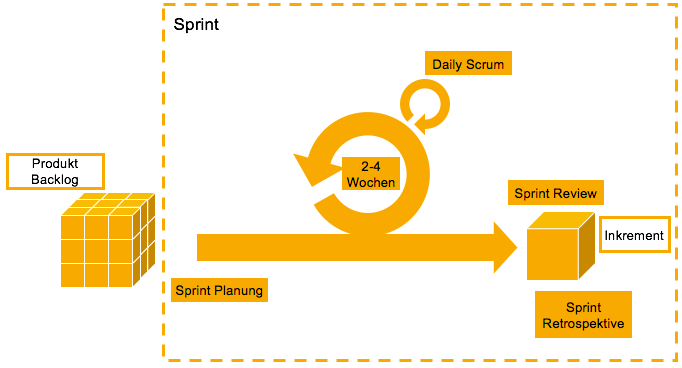
\includegraphics[width=11cm]{Abbildungen/scrum}
                        \caption{Planungszyklus Scrum\protect\footnotemark}
                        \label{abb:scrum}
                        \end{center}
                  \end{figure}

                  \footnotetext{Eigene Grafik erstellen!}

                Während des Sprint werden keine weiteren Themen zum Scope ergänzt und weder Zeit- noch Qualitätsplanung angepasst. Erst die Sprint-Planung am Ende jedes Zyklus bietet die Möglichkeit zur Nachkalibration. Die Dauer eines Sprints ist daher auch so gewählt, dass das Projekt flexibel genug ist um auf Anforderungen einzugehen, die Entwickler allerdings die Chance erhalten sich voll und ganz auf eine Aufgabe zu konzentrieren und nicht ständig durch Anforderungsänderungen aus ihrem Fokus gerissen werden. Im Folgenden werden die vier Phasen eines Sprints weiter aufgeschlüsselt:

                Das \emph{Sprint Planning} dient als Vorbereitung für den kommenden Sprint. Im Zentrum des Planungsprozesses stehen zwei Fragen, die am Ende des Meetings beantwortet sein sollen.
                \begin{itemize}
                  \item Was kann in diesem Sprint fertiggestellt werden?
                  \item Wie wird die ausgewählte Arbeit erledigt?
                \end{itemize}

                In der ersten Phase präsentiert der Product Owner die Wünsche des Kunden und nennt priorisiert alle Dinge, die bis zum Ende des Sprints geschafft werden sollten. Das Entwicklungsteam diskutiert mit ihm daraufhin, ob die Zeitplanung und Deadlines realistisch sind, oder ob es denkt deutlich mehr bzw. deutlich weniger zu schaffen. Haben sich Product Owner und Scrum Team auf einen Scope geeinigt kommt es zu Phase zwei des Sprint Planning, in der geplant wird, wie das Sprint-Ziel zu erreichen ist.

                Die Vorgehensweise stellt bei Software beispielsweise grob die Codestruktur dar mit Methoden, Eigenschaften von Klassen usw. Sie lässt sich beispielsweise durch UML-Klassendiagramme sehr gut erfassen. Hierbei sollen unabhängig von Kompetenzen und Erfahrungen alle Ideen des Teams eingebracht werden. Ein großes Problem bei Sprint Plannings sind häufig Externe, insbesondere Vorgesetzte, die bei jungen Entwicklerteams oft Ratschläge geben, die aber als Weisung aufgenommen werden. Durch die Präsenz weisungsbefugter Personen wird die Kreativität im Team so häufig untergraben und nicht vollkommen ausgeschöpft.
                Der Scrum Master hat zusätzlich noch die Aufgabe sehr dominante und aktive Personen zu bremsen und auch die ruhigeren Charaktere in die Diskussion mit einzubinden. Während des Sprint Plannings und auch dem gesamten Sprint fungiert er als Moderator.\footnote{Vgl. Maximini, 2013, S.182f.}

                Das \emph{Daily Scrum} findet Arbeitstäglich statt, dauert meist 15 Minuten und ist ein Meeting mit dem gesamten Team. Um Dynamik zu erzeugen und nicht zu überziehen findet es meist im stehen kurz vor der Mittagspause statt. Das Daily Scrum dient dazu dem gesamten Entwicklungsteam eine Übersicht zu geben, wer wo steht und wie weit man als Team bei der Verwirklichung des Sprint Ziels ist. Außerdem findet man häufig eine Lösung, wenn Probleme auftreten und diese im Team vorgestellt werden. Jedes Mitglied des Scrum-Teams ist nacheinander an der Reihe und beantwortet in der großen Runde folgende drei Fragen:

                \begin{itemize}
                  \item Was habe ich gestern getan?
                  \item Was werde ich bis morgen tun?
                  \item Wo bin ich dabei auf Hindernisse gestoßen?
                \end{itemize}

                Insbesondere bei der letzten Frage geht es nicht darum Lösungen während des Daily Scrums zu finden, sondern im Scrum das Problem vorzustellen und jemanden zu finden, der es im Anschluss gemeinsam mit angeht. Somit schweift das Team gedanklich nicht ab, sobald es technischer wird. Dem Daily Scrum kommt somit eine Planungs- und Kontrollfunktion zu \footnote{Vgl. Maximini, 2013, S.183.}.

                Der \emph{Sprint Review} schließt sich an einen Sprint an, um auf Grundlage der Ergebnisse erneut zu planen. Beim Sprint Review sind neben dem gesamten Scrum-Team auch Stakeholder anwesend, denen das Produkt vorgestellt werden soll. Dabei ist wünschenswert, dass die Stakeholder das Produkt selber testen können und die Entwickler dabei die Wünsche und Gedanken der Stakeholder zum Produkt notieren. Auf Grundlage dieses Feedbacks wird anschließend das Produkt kontrolliert und falls nötig der Backlog erweitert.

                Auf Grundlage der Definition von Done werden im Sprint Review die Backlog einträge abgehakt, die erfüllt worden und die bestehenden Einträge auf Zeit und Erreichbarkeit überprüft. Das Sprint Review stellt somit die Grundlage zum kommenden Sprint Planning dar.\footnote{Vgl. Scrum Guide, 2013, S..}

                Die \emph{Sprint Retrospektive} stellt das Pendant zum Sprint Planning dar und schließt einen Sprint formell ab. Während beim Sprint Review das erstellte Produkt im Mittelpunkt steht betrachtet die Sprint Retrospektive die Zusammenarbeit des Scrum Teams und dessen Arbeitsweise. Das Ziel dieses Meetings ist es Maßnahmen herauszuarbeiten, wie die Zusammenarbeit im Team verbessert werden kann oder wie die Qualität der Endprodukte verbessert werden kann. Am Ende des Meetings soll eine Liste mit wenigen, aber greifbaren Maßnahmen stehen, die jedes Teammitglied bis zum Ende des folgenden Sprints umsetzen kann.\footnote{Vgl. Scrum Guide, 2013, S.13.}

                Scrum ist eines der bekanntesten agilen Verfahren und wird häufig als Synonym für eine agile Vorgehensweise genutzt. Es gibt Vorgaben zum Management von Anforderungen und lässt den Entwicklerteam freien Spielraum zur Umsetzung eben dieser. Scrum-Teams bemühen sich aus jedem Sprint etwas zu lernen und ihre Vorgehensweise im nächsten Sprint anzupassen um sich kontinuierlich zu verbessern.

%----------------------------------
%
% Qualitätssicherungsmodelle
%
%----------------------------------
    \section{Qualitätssicherungsmodelle}

        Um das Ziel der Qualitätssicherung zu verstehen wird die Qualitätssicherung zunächst vom Qualitätsmanagement abgegrenzt. Das Qualitätsmanagement stellt alle Maßnahmen zur Führung und Steuerung der Qualität im Unternehmen dar, während die Qualitätssicherung nach ISO 9000 als \enquote{Teil des Qualitätsmanagements definiert, der durch das Erzeugen von Vertrauen darauf gerichtet ist, dass Qualitätsanforderungen erfüllt werden.} Dabei geht es nicht darum ein Produkt kontinuierlich zu verbessern, sondern ein vorgegebenes Niveau zu erreichen oder zu halten.\footnote{ANGABE SUCHEN}

        \begin{quote}
          Die Darlegung des Qualitätsmanagements, d.h. alle Tätigkeiten zur Schaffung von Vertrauen, dass die Qualitätsanforderungen erfüllt werden, wird Qualitätssicherung genannt. Als zentrale Maßnahmen braucht es regelmäßige Überprüfungen, ob das Qualitätsmanagementsystem wie geplant funktionert und ob die vorgesehenen Qualitätsmaßnahmen wirklich durchgeführt werden. Solche Überprüfungen heißen Audits.\footnote{Glinz, 2005, S.120.}
        \end{quote}

        Im Projekt unterscheidet man außerdem zwischen organisatorischen, analytischen und konstruktiven Maßnahmen zur Sicherung der Qualität. Diese werden im Folgenden definiert:

        \begin{description}
          \item[Organisatorische Maßnahmen] Definiert die Aufbau- und Ablauforganisation , die die Softwarequalität im Projekt verankert. Dies schafft die Voraussetzung dafür, dass analytische und konstruktive Maßnahmen durchführbar und wirksam sind.
          \item[Analytische Qualitätssicherung] In analytischen Verfahren wird ein bereits fertiger Prüfling untersucht, um Fehler zu finden. Analytische Maßnahmen wirken sich auf die Softwarequalität indirekt aus, wenn nämlich die gefundenen Fehler beseitigt werden.
          \item[Konstruktive Qualitätssicherung] Maßnahmen, die bereits bei der Konstruktion von Software auf die Verbesserung ausgewählter Qualitätsaspekte abzielen und nicht erst nachträglich durch Prüfung und Korrektur.
        \end{description}

%        Zu den organisatorischen und analytischen Maßnahmen wird im Folgenden nur ein kurzer Überblick zu einem anerkannten, ausgewählten Modell gegeben um den Fokus auf konstruktive, vorausschauende Maßnahmen zu legen. Fehler, die frühzeitig, also vor der Implementierung bzw. Umsetzung, erkannt werden sind aufgrund des Zehnermodells (\emph{Grafik mit 10x Preiserhöhung je später Fehler erkannt wird}) deutlich günstiger zu beheben, als nachträglich erkannte Fehler.

        \subsection{Beispiel organisatorischer Qualitätssicherungsmaßnahmen}

            Qualität im Projekt muss durch drei stellen umgesetzt werden und zwar in der Aufbauorganisation, der Ablauforganisation und in Form eines Qualitätsmanagementsystems.

            \subsubsection{Aufbauorganisation}

                Die Aufbauorganisation bezieht sich dabei auf die Ansiedlung der Qualitätssicherung im Organisationsdiagramm des Unternehmens. Bei einer klassischen, hierarchieschen Struktur ist es zwingend erforderlich, dass die Qualitätsbeauftragten auf allen Hierarchieebenen vertreten sind, ohne, dass die normalen Projektteilnehmer eine Weisungsbefugnis gegenüber diesen haben.\footnote{Vgl. Schneider, 2007, S.12f.}

                Das Qualitätsteam bekommt \enquote{Narrenfreiheit}, was ihnen erlaubt offen Kritik zu üben, ohne Konsequenzen fürchten zu müssen. Diese sollte allerdings gerechtfertigt sein und die negative Konnotation, dass die Narrenfreiheit \enquote{Dümmlichkeit} impliziert, entfällt.\footnote{Hier noch eine Grafik der Organisation?}

                Mit Hilfe dieser Struktur wird verhindert, dass Qualitätsverantwortliche durch Druck ihrer Vorgesetzten die eigenen Ansprüche herunterschrauben, da Deadlines oder Budgetziele andernfalls nicht haltbar wären.\footnote{Vgl. Schneider, 2007, S.13.}

            \subsubsection{Ablauforganisation}

                \begin{quote}
                  Innerhalb der Ablauforganisation muss das Qualitätsmanagementsystem für alle Abläufe die qualitätsrelevanten Kompetenzen, Verantwortlichkeiten und gegenseitigen Beziehungen festlegen. Man ist dabei bestrebt, möglichst wenig Qualitätsaufgaben separat zu regeln, sondern diese weitestgehende in die Prozesse des Unternehmens zu integrieren.\footnote{Glinz, 2005, S.119.}
                \end{quote}

                Damit wird gesagt, dass der Qualitätsprozess nicht einsam und für sich stehen soll, sondern eine enge Verwebung mit den bestehenden Prozessen des Unternehmens angestrebt wird. Die Qualitätsprozesse sind unterstützend zum Entwicklungsprozess der Software, da mit qualitativer Software und keine qualitativen Softwareentstehungsprozess Geld verdient werden kann. Der Qualitätsprozess dient somit zur Unterstützung der Projektprozesse.

            \subsubsection{Qualitätsmanagementsystem}

                Das Qualitätsmanagementsystem sind nach ISO 8402 alle
                \begin{quote}
                    zur Verwirklichung des Qualitätsmanagements erfoderliche Organisationsstruktur, Verfahren, Prozesse und Mittel.\footnote{ANGABE SUCHEN. $\rightarrow$ Schneider?}
                \end{quote}
                Dies steht in direkter Verbindung mit der ISO 8402 Definition des Qualitätsmanagements: \begin{quote}
                    Alle Tätigkeiten der Gesamtführungsaufgabe, welche die Qualitätspolitik, Ziele und Verantwortlichkeiten festlegen sowie diese durch Mittel wie Qualitätsplanung, -lenkung, -sicherung und -verbesserung im Rahmen des Qualitätsmanagementsystems verwirklichen.\footnote{ANGABE SUCHEN $\rightarrow$ Schneider?}
                \end{quote}

                Das Ziel des Qualitätsmanagementsystems ist eine Verbesserung des gesamten Unternehmens auf der Prozess bzw. Produktebene. Auf Software angewandt bedeutet dies, dass das Qualitätsmanagementsystem sicherstellt, dass die Software alle internen und externen Ansprüche erfüllt. Dabei ist Qualität kein Selbstzweck, sondern dient stets der Verbesserung des Produkts.

        \subsection{Beispiel analytischer Qualitätssicherungsmaßnahmen}
        \label{subsec:analytischeqs}

            Analytische Qualitätssicherungsmaßnahmen beziehen sich auf Schritte die nach der Entwicklung einer Software darauf abzielen die korrekte Funktion eben dieser sicherzustellen. Das bedeutet insbesondere, dass neben einer aktuellen Dokumentation eine Menge von Tests durchgeführt werden müssen, die überprüfen, ob die Software auf Eingaben mit den erwarteten Ausgaben reagiert. Die länge Testphase, die sich an die Entwicklung anschließt kann oft nicht korrekt festgelegt werden, da nicht abzusehen ist, wie viel Code korrigiert werden muss und wie schwerwiegend die Fehler sind. Somit gefährdet die Testphase meist die vorher festgelegte Projektlaufzeit und das Projektbudget.

            Obwohl die Testphase häufig unerwünscht ist, ist sie essentiell, da Fehler die noch während des Projekts entdeckt werden günstiger zu beheben sind als im späteren Verlauf. Je nach Einsatzgebiet der Software kann ein Fehler der Software die Kosten des Testvorgangs weit übersteigen.
            Aufgrund dessen sollte jedes Teilprodukt einer Software so früh wie möglich geprüft werden.\footnote{Prechelt, 2010, S..}

            Ein Test ist nach IEEE Standard 610.12 definiert als:
            \begin{itemize}
              \item \enquote{The process of operating a system or component under specified conditions, observing or recording the results, and making an evaluation of some aspect of the system or component.}
              \item \enquote{The process of analyzing a software item to detect the differences between existing and required conditions (that is, bugs) and to evaluate the features of the software items.}\footnote{IEEE 610.12, 1990, S.20.}
            \end{itemize}

            Testen ist daher die Anwendung der Software mit dem Ziel diese zum Absturz oder zu einer falschen Ausgabe zu führen um diese Fehler zu dokumentieren.
            Um möglichst viele Fehler und Probleme abzudecken existiert eine große Menge an Testverfahren. Diese werden in Dynamische Verfahren und Statische Verfahren unterteilt. Die dynamischen Verfahren haben gemein, dass die Software im Rahmen des Tests ausgeführt wird und mit verschiedenen Parametern und auf verschiedenen Laufzeitumgebungen ausgeführt wird. Bei statischen Testverfahren wird der Programmcode geprüft, ohne das dieser ausgeführt wird. Bei der statischen Analyse wird auf die Einhaltung von Standards geprüft und es werden Statistiken zum Quellcode erstellt, die beispielsweise Verzweigungen und die Codezeilenanzahl dokumentieren. Dynamische Tests prüfen dagegen eine Vielzahl von Anwendereingaben und Parametern um mögliche Fehler zu finden. Nachfolgend sind eine Menge von dynamischen und statischen Testverfahren gelistet. Beispiele für die beiden Kategorien werden im Anschluss betrachtet.

            \begin{itemize}
              \item Dynamische Verfahren (Test)
                \begin{itemize}
                  \item Defekttest
                  \item Benutzbarkeitstest
                  \item Lasttest
                  \item Akzeptanztest
                \end{itemize}
              \item Statische Verfahren
                \begin{itemize}
                  \item Manuelle Verfahren (Durchsichten, Inspektionen)
                  \item Automatische Verfahren (Modellprüfung, Quelltextanalyse)
                \end{itemize}
            \end{itemize}

            \subsubsection{Strukturtest}
                Ein Strukturtest, auch \emph{White Box/Glass Box Test} genannt, betrachtet Testfälle auf Grundlage der Implementation einer Komponente.
                Dies bedeutet, dass nicht nur eine klassische Funktion aus Anwenderperspektive gestartet wird, sondern dass die Bestandteile des Codings überprüft werden. Die geschieht auf bis zu vier Ebenen:
                \begin{itemize}
                  \item Anweisungsüberdeckung ($C_0$)
                    \begin{itemize}
                      \item Jede Anweisung wurde mindestens einmal ausgeführt
                      \item Für Fehlerbehandlungscode meist schwierig oder sogar unmöglich
                    \end{itemize}
                  \item Bedingungsüberdeckung ($C_1$)
                    \begin{itemize}
                      \item Zusätzlich: Jede Steuerbedingung (bei if, while, switch etc.) war mindestens einmal falsch und einmal wahr
                    \end{itemize}
                  \item Schleifenüberdeckung ($C_2$)
                    \begin{itemize}
                      \item Zusätzlich: Jede Schleife wird einmal 0-fach, einmal 1-fach und einmal mehrfach durchlaufen
                    \end{itemize}
                  \item Datenflusskriterien
                      \begin{itemize}
                        \item Viele verschiedene Kriterien der Art: \enquote{Jedes Beschreiben einer Variable wird auch später mal ausgelesen/benutzt}
                      \end{itemize}
                      \footnote{Prechelt, 2010, S..}
                \end{itemize}

            \subsubsection{Funktionstest}
                Das Gegenteil des Strukturtests stellt der Funktionstest dar. Dieser wird auch \emph{Black Box Text} genannt, da nur Ein- und Ausgaben betrachtet werden. Wie die Eingaben im Programm verarbeitet werden wird im Strukturtest geprüft.

                Die Herausforderung des Funktionstests ist es vorab das erwartete Resultat festzulegen, das bei eine Buchhaltungssoftware sehr kompliziert und umständlich zu errechnen sei. Im besten Fall werden die erwarteten Resultate schon vor der Implementierung festgelegt, um eine Referenz zur Funktionsfähigkeit des Programms festzulegen. Dies wird beispielsweise bei Unit-Tests angewandt, die eine kleine Teilkomponente eines Programms ausführen und mit einem gewünschten Ergebnis gegenprüfen.

                Außerdem muss jede Art des Verhaltens getestet werden. Dazu gehören erwartete Werte, Fehlerfälle und Grenzwerte (Sehr große oder kleine Zahlen).\footnote{Vgl. Prechelt, 2010, S..}

        \subsection{Beispiel konstruktiver Qualitätssicherungsmaßnahmen}

%            \begin{quote}
%              Oft wird er beim testen die Spezifikation richtig geklärt (Was wird erwartet, wenn ich XY drücke/tue). Solche Fälle schon beim Entwurf von Software planen und festlegen! Doku nachbessern\footnote{Prechelt FU Berlin}
%            \end{quote}
            \begin{quote}
                Eine Technik, eine Maßnahme, ein Teilprodukt oder ein Prozess werden konstruktiv zur Qualitätsverbesserung eingesetzt, weil man aus erfahrung weiß, dass sie sich dafür schon bewährt haben, und wo das gelungen ist.\footnote{Schneider, 2007, S.179.}
            \end{quote}

            Das Ziel von konstruktiven Maßnahmen ist es nicht nur Fehler zu entdecken und nachträglich auszubessern, sondern die Entstehung von Fehlern schon frühzeitig zu verhindern. Dies kann durch anerkannte Normen, Best-Practices aus alten Projekten oder durch Erfahrung im Umgang mit Projekten erreicht werden. Außerdem sollten bei erkannten Fehlern im Produkt nicht bloß nachgebessert, sondern auch die Ursache des Fehlers aufgedeckt und behoben werden.

%            Dies entspricht den Vorgaben des Kaizen, der ständigen Verbesserung.


        \subsection{Ausgewählte Methoden der Qualitätssicherung}

            \subsubsection{ISO 9000}

            Die ISO 9000er Normen umfassen die ISO 9000 bis 9004. Die ISO 9001 bis 9003 enthalten dabei konkrete Anforderungen an das Qualitätsmanagement im Unternehmen, während die ISO 9000 und 9004 als Leitfaden dienen sollen. Die Unterschiede zwischen den Normen 9001 bis 9003 werden im Folgenden kurz dargestellt:
            \begin{itemize}
              \item Die ISO 9001 umfasst das Qualitätsmanagement des gesamten Unternehmens inklusive Entwicklung, Konstruktion, Produktion, Montage und Kundenservice. Die ISO 9001 umfasst alle Anforderungen der Normen ISO 9002 und 9003 und ist somit die vollständigste und weitgreifendste. Im Rahmen dieser Arbeit wird die ISO 9001 betrachtet.
              \item Eine Zertifikation nach ISO 9002 gewährleistet geprüfte Prozesse in Produktion und Montage.
              \item Die ISO 9003 betrifft Endprüfungen von Produkten.
            \end{itemize}

            Die ISO 9001 gibt jedoch keine konkreten Werkzeuge und Methoden vor um Qualität zu erreichen, sondern nur wofür Modelle vorgelegt werden müssen und was zu dokumentieren ist. Anhand dieser Standards kann das vorhandene Qualitätsmanagement eines Unternehmens lediglich bewertet und zertifiziert werden.

            Die Inhaltsübersicht der ISO 9001  stellt eine Anforderungsübersicht zum Qualitätsmanagement einer Organisation dar. Die Kapitel 4 bis 8 des Standards betreffen jeweils ein Element, dass zwingend erforderlich ist um eine Zertifizierung zu erhalten.

            Zunächst wird ein Qualitätsmanagementsystem gefordert. \enquote{The organization shall establish, document, implement and maintain a quality management system and continually improve its effectiveness in accordance with the requirements of this international standard\footnote{ISO 90003, 2008, S.5.}.}
            Die Definition eines Qualitätsmanagementsystems ist oben gegeben.

            Im Anschluss daran wird gefordert, dass sich das Management zur Implementierung des Qualitätsmanagementsystems bekennt und seine Unterstützung beweisen kann. Dies geschieht vorrangig durch Kommunikation zur Belegschaft, Gespräche mit dem mittleren Management und Bereitstellung der Ressourcen. Das gesamte fünfte Kapitel der ISO 9001 beinhaltet die Verantwortung des Managements.

            Daran angeschlossen wird ein Ressourcenmanagement gefordert, dass die benötigten Mittel festlegt und sicherstellt, dass diese vorhanden sind. Dabei sind neben Infrastruktur und Produktionsmitteln auch humane Ressourcen gefordert.

            Kapitel 7 behandelt die Produktrealisierung vom Design bis hin zur Endverarbeitung und behandelt somit den in ISO 9002 behandelten Produktionsprozess.

            Zuletzt wird die Kontrolle, Analyse und Verbesserung behandelt. Das Ziel ist zu zeigen, dass das Produkt die gestellten Anforderungen erfüllt und zu prüfen, dass alle etablierten Prozesse geeignet sind um die Qualität zu gewährleisten. Außerdem sollen Möglichkeiten gefunden werden den gesamten Entwicklungsprozess zu verbessern.

            Die ISO 9001 gibt zudem den Deming-Zyklus als Modell vor. Dieser sieht vier Schritte vor, die iterativ durchlaufen werden, um optimale Qualität zu gewährleisten.
            \begin{itemize}
              \item Plan
              \item Do
              \item Check
              \item Act
            \end{itemize}
            Zunächst soll geplant werden, wie der Prozess bzw. das Endprodukt, die Software, aussehen soll um danach die geplanten Prozesse zu durchlaufen. Am Ende dieser Durchläufe folgt die Prüfungsphase in der mit statistischen Methoden kontrolliert wird, ob die in der Planungsphase gesteckten Anforderungen erfüllt wurden. Auf Grundlage dieser Ergebnisse werden Maßnahmen beschlossen um die Prozesse und Produkte zu optimieren und somit einen kontinuierlichen Verbesserungsprozess im Unternehmen zu etablieren.

            \subsubsection{Total Quality Management}

            Total Quality Management ist ein umfassendes Managementkonzept, dass die Grundlage für viele heute existierende Qualitätsmanagementsmodelle bildet. Es betrachtet neben den Anforderungen der Kunden und Mitarbeiter an die Qualität der Software, die Belange aller Stakeholder und die der Gesellschaft. Außerdem prüft es nicht nur die Eignung der Prozesse um zum Ergebnis zu kommen, sondern auch die tatsächlich resultierten Ergebnisse.\footnote{Vgl. http://www.olev.de/t/tqm.htm, 2016.}

            \subsubsection{Six Sigma}
            \label{subsec:sixsigma}

            Das Ziel Six Sigmas ist es \enquote{die Anforderungen des Kunden vollständig und profitabel [zu] erfüllen}\footnote{Knöfel, 2009, S. 7}. Dabei ist neben dem externen Kunden, dem Abnehmer des Endprodukts, auch jeder interne Abnehmer eines Produktes gemeint. Sollte Abteilung B eines Unternehmens eine Fertigung von Abteilung A des gleichen Unternehmens weiterverarbeiten, so ist Abteilung B im Six Sigma Modell Kunde der Abteilung A. Auf diese Weise soll entlang der gesamten Prozesskette die Fehlerzahl gegen Null laufen.

            Six Sigma ist eine Methode um möglichst perfekte Prozesse zu etablieren. Der Name dieser Methode entstammt der Statistik und entspricht der Zahl der Annahmequote von $6\sigma = 99.99966\%$. Dies bedeutet, dass beim Durchlauf von 1 Millionen Prozessen, bzw. bei 1 Millionen Endprodukte lediglich 3,4 fehlerhaft sind. Dies entspricht einer Fehlerquote von praktisch Null.\footnote{Vgl. Knöfel, 2009, S.20f.}

            Diese Werte werden anhand der Gaußschen Glockenkurve festgelegt und entsprechen der Abweichung zum Erwartungswert.

            \begin{figure}[!htbp]
                \begin{center}
                    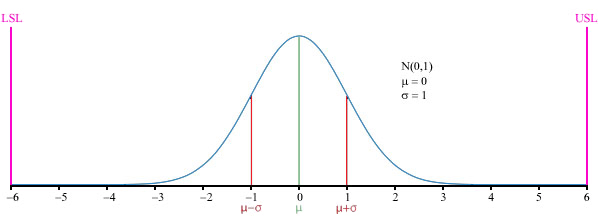
\includegraphics[width=11cm]{Abbildungen/sixs_normalverteilung}
                    \caption{Gaußsche Normalverteilung\protect\footnotemark}
                    \label{abb:normalverteilung}
                \end{center}
            \end{figure}

            \footnotetext{http://www.wikiwand.com/de/Six\_Sigma}

            Um die Abweichungen zum Zielwert möglichst gering zu halten wird der Deming-Kreis, der im ISO 9001 Kapitel vorgestellt wurde, erweitert. Six Sigma verwendet den sogenannten DMAIC Verbesserungsprozess - Define, Measure, Analyse, Improce, Control - der aus dem Kaizen Prinzip (Kai - Veränderung, Zen - Zum Besseren) aus Japan entwickelt wurde. Der DMAIC Prozess wird durchlaufen, bis die Anforderungen des Kunden erfüllt wurden.

            Zunächst wird die Problemstellung definiert. Das bedeutet, dass der Kunde befragt werden muss, welche Anforderungen er an den Prozess hat und welche Ausschuss- bzw. Fehlerrate er akzeptieren würde. Dies ist die Zielsetzung für den nachfolgenden Zyklus.

            Daraufhin wird das Maß festgelegt, an dem das Endergebnis gemessen wird. Die zuvor aufgenommenen Kundenanforderungen werden in statistische Messgrößen übersetzt und die zu messenden Kennzahlen festgelegt.
            Während eines Prozessdurchlaufs werden nun Messdaten erfasst und gespeichert.

            Die erfassten Daten werden nun analysiert und die Ursache der Abweichungen vom Zielwert wird erfasst.

            Auf Grundlage dieser Abweichungen werden Verbesserungsvorschläge erarbeitet und der Mehrwert eben dieser wird beziffert. Zu beachten ist, dass die Ursache bekämpft werden sollte und nicht die Symptome.

            Zuletzt werden Steuerungs- und Kontrollmöglichkeiten eingeführt, damit der verbesserte Prozess nachhaltig und konsistent umgesetzt wird. Das Six Sigma Team zieht sich zurück und überlässt die Kontrolle und den Prozess der ausführenden Abteilung.\footnote{Vgl. Knöfel, 2009, S. 37.} 
    \chapter{Qualitätsmerkmale von Software}
\label{cha:qualitaetsmerkmale}

%----------------------------------
%
% Definition von Qualität
%
%----------------------------------
    \section{Definition von Qualität}
    \label{sec:definitionQualitaet}

        Der Begriff Qualität wird im Alltag häufig und in verschiedenen Situationen verwendet. Daher soll hier eine Grunddefinition des Qualitätsbegriffs gegeben werden, der im Rahmen der vorliegenden Arbeit verwendet wird.

        Es kann gesagt werden, dass Qualität
            \begin{itemize}
                \item \enquote{eine Menge von Eigenschaften repräsentiert, die einem Produkt oder Verfahren immanent oder beigegeben ist.
                \item einer der Maßstäbe ist, mit dem der Kunde seine Kaufentscheidung herbeiführt.
                \item ein Faktor ist, der in intensiver Wechselwirkung mit der Wettbewerbssituation und Leistungsfähigkeit eines Anbieters steht.}\footnotemark
            \end{itemize}

            \footnotetext{Pfeifer (Qualitätssicherung).}

        Dies verfeinert die Definition der \emph{International Organisation for Standardization} (ISO) 9000: \enquote{Qualität ist der Grad, in dem ein Satz inhärenter Merkmale Forderungen erfüllt.}\footnote{Glinz (Software Engineering), S.115.} Für Qualität bedeutet das, dass einem Werksstück, Prozess oder auch einer Software messbare und nicht messbare Eigenschaften inne wohnen. Bei Software unterscheidet man beispielsweise zwischen messbaren, funktionalen Anforderungen und nicht messbaren, nicht funktionalen Anforderungen. Ein Beispiel für eine funktionale Anforderung ist die Antwortzeit eines Programms, während ein gutes User Interface einer nicht funktionalen Anforderung entspricht. Inhärent sind Merkmale, die sich nach Auslieferung nur sehr schwer oder gar nicht verändern lassen, während der Preis als Beispiel für ein nicht-inhärentes Merkmal sehr frei zu gestalten ist.

        Ein wichtiges Merkmal der vorausgegangenen Definition ist allerdings die Qualität als Merkmal der Kundenbeeinflussung. Dabei stellt sie sich als Merkmal dar, dass für oder auch gegen die Kaufentscheidung eines bestimmten Produktes spricht. Als Softwarehersteller ist somit eine Sicherung der Qualität unumgänglich, um nachhaltig am Markt zu agieren.

        So wird Qualität im Rahmen dieser Arbeit als eine Eigenschaft des fertigen Produkts, in diesem Fall der Software, angesehen, die nachträglich nur durch sehr viel Aufwand verändert werden kann. Qualität ist ein Maßstab auf dessen Grundlage Kunden eine Kaufentscheidung treffen, abhängig davon, ob die eigenen Anforderungen an das Produkt erfüllt sind.

%----------------------------------
%
% Vorstellung der Qualitätsmerkmale
%
%----------------------------------
    \section{Vorstellung der Qualitätsmerkmale}
    \label{sec:vorstellungMerkmale}

        Die Produktqualität ist, wie zuvor gezeigt, ein wichtiges Merkmal zum Bilden und Fortbestehen eines Unternehmens. Im Folgenden soll die Qualität einer Software messbar gemacht werden.

        Die ISO 9126 stellt hierzu sechs Charakteristiken bereit, auf deren Grundlage die Qualität von Software bewertet werden kann. Die Charakteristiken sind zusätzlich in insgesamt 27 Unterdimensionen untergliedert. Es werden nun alle Obercharakteristiken betrachtet und im Anschluss drei Merkmale ausgewählt, die im Rahmen dieser Arbeit betrachtet werden. Die Definitionen der Unterdimensionen befinden sich im Glossar.

        \subsection{Funktionalität}

            \begin{quote}
              \enquote{The capability of the software product to provide functions which meet stated and implied needs when the software is used under specified conditions.}\footnote{ISO 9126-1 (Information technology), S.7.}
            \end{quote}

            Die Charakteristik \emph{Funktionalität} gibt den Einsatzzweck der Software an. Beispielsweise ist eine Funktionalität einer Buchhaltungssoftware die Berechnung einer Gewinn- und Verlustrechnung. Im Gegensatz zu den folgenden Charakteristiken gibt diese an, was die Software tut, anstatt zu sagen, auf welche Weise sie etwas tut.

            Darunter fallen die Abdeckung der gestellten Anforderungen an Funktionalität und Genauigkeit, sowie Sicherheitsaspekte.\footnote{Vgl. ISO 9126-1 (Information technology), S.8.} Im Falle der SAP SE hat ein Softwareprodukt beispielsweise die Funktion der Geschäftspartnerverwaltung und sollte somit alle fachlich an sie gestellten Anforderungen bedienen. Außerdem sollte bei einer identischen Eingabe stets ein identisches, erwartetes Resultat entstehen. Durch den Scope (engl. für Umfang), der zu Beginn eines Projektes erstellt wird, ist diese Charakteristik meist schon zu Beginn eines Projekts genau spezifiziert.

        \subsection{Verlässlichkeit}

            \begin{quote}
              \enquote{The capability of the software product to maintain a specified level of performance when used under specified conditions.}\footnote{ISO 9126-1 (Information technology), S.8.}
            \end{quote}

            Die Charakteristik \emph{Verlässlichkeit} gibt die Fähigkeit einer Software an, unter den festgelegten Umweltbedingungen immer in einem vorher festgelegten Rahmen zu reagieren. In mittlerweile veraltetenen Definitionen der ISO Normen bezieht sich die Verlässlichkeit darauf, eine bestimmte, benötigte Funktion auszuführen.

            Das Ziel der Entwickler ist eine Software, die jederzeit in dem erwarteten Umfang reagiert und falsche Eingaben, falsche Benutzungsanweisungen und ungültige Datensätze verkraftet oder verhindert. Software ist genau dann verlässlich, wenn keine Fehler durch Defekte in dieser auftreten, keine Angriffe, bewusst oder unbewusst, von außen oder innen möglich sind und sämtliche Daten auch nach einem Systemabsturz wieder herstellbar sind.\footnote{Vgl. ISO 9126-1 (Information technology), S.9.}

            Unternehmen der Finanzindustrie stellen hohe Anforderungen an die Verlässlichkeit ihrer IT Systeme. Ebenso ist die zuverlässige Ausführung von Prozessen bei der Verarbeitung von Zahlungsströmen u.ä. unverzichtbar.
            Derzeit werden Softwarelandschaften eingesetzt, die in den 1970er Jahren aufgebaut wurden und seitdem im Stand gehalten und erweitert werden.\footnote{Vgl. TOGAF/Bian (Integrating TOGAF with BIAN), S.10.} Die auf Mainframes\footnote{Siehe Glossar.} aufgebauten Architekturen sind sehr teuer in der Wartung und Instandhaltung, aber gewährleisten eine hohe Verfügbarkeit von bis zu 99.999\%.\footnote{Vgl. Symonds (Mainframes), S.12.}
            %Dies bedeutet, dass ein Mainframe nur circa 5,26 Minuten pro Jahr nicht zu erreichen ist. IBM gibt für ihre Mainframes zudem eine durchschnittliche Zeit zwischen Fehlern von 20 bis 30 Jahren an. Außerdem werden Operationen häufig mehrfach gleichzeitig durchgeführt und die Ergebnisse verglichen. Somit sind fehlerhafte Berechnungen nahezu ausgeschlossen.

        \subsection{Benutzerfreundlichkeit}

            \begin{quote}
              \enquote{The capability of the software product to be understood, learned, used and attractive to the user, when used under specified conditions.}\footnote{ISO 9126-1 (Information technology), S.9.}
            \end{quote}

            \emph{Benutzerfreundlichkeit} sagt aus, dass ein fachlich versierter Anwender intuitiv die Funktion des Programms erkennt und es verwenden kann. Dabei soll der Anwender nach Möglichkeit ein gutes Gefühl haben und die Software als schön bezeichnen.

            Aus dem Privatleben sind geschäftliche Anwender inzwischen einfache, intuitive Oberflächen gewöhnt und tragen diese Anforderung ins Unternehmen.\footnote{Vgl. CITO Research (Business Intelligence), S.1.} Außerdem werden mehr mobile Geräte in Unternehmen verwendet. Um alle Daten, zu jeder Zeit und an jedem Ort zur Verfügung zu haben, werden die Daten häufig in der Cloud\footnote{Siehe Glossar.} bereitgestellt und über webbasierte Applikationen angezeigt.

            Die SAP SE verfolgt die Strategie, dass sich die Oberflächen zwischen mobilen Geräten und Computern nicht unterscheiden und keine Daten auf dem Gerät liegen. Durch einheitliche Oberflächen soll die Produktivität der Nutzer erhöht werden und die Einarbeitungszeit reduziert werden.
            Das Ziel der SAP SE ist es, durch eine intuitive Menüführung beim Endbenutzer einen Produktivitätszuwachs zu erreichen, dadurch, dass dieser schnell und sicher durch die Oberfläche navigieren kann. Durch leicht verständliche Oberflächen soll zudem die zur Einarbeitung benötigte Zeit reduziert werden. Somit wird im Idealfall der Schulungsbedarf des Kunden reduziert.\footnote{Vgl. Deck (User Interface Technologies), S.14ff.}

        \subsection{Effizienz}

            \begin{quote}
              \enquote{The capability of the software product to provide appropriate performance, relative to the amount of resources used, under stated conditions.}\footnote{ISO 9126-1 (Information technology), S.10.}
            \end{quote}

            Der Faktor \emph{Effizienz} drückt das Verhältnis zwischen der Performanz der Software und den dafür verbrauchten Ressourcen aus.\footnote{Vgl. ISO 9126-1 (Information technology), S.10.} Die Effizienz steigt, wenn die Performance bei gleichbleibendem Ressourcenverbrauch steigt, oder, wenn bei gleichbleibender Performance der Ressourcenverbrauch sinkt und umgekehrt.

            Um selbst bei umfangreichen Datenabfragen und Berechnungen eine geringe Antwortzeit zu gewährleisten verfolgt die SAP SE den Trend der In-Memory Datenhaltung. Die SAP SE verwendet hierzu die Datenbanktechnologie \emph{High-Performance Analytical Appliance} (HANA)\footnote{Siehe Glossar.}. Trotz der gestiegenen Ressourcennutzung ist der Performance Gewinn größer, um deren Verwendung zu rechtfertigen. Gerade im Umgang mit Massendaten, die im Finanzbereich anfallen ist eine effiziente Datenhaltung und Verarbeitung sehr wichtig.\footnote{Vgl. SAP SE (HANA in Banking), S.5.}

        \subsection{Wartbarkeit}

            \begin{quote}
              \enquote{The capability of the software product to be modified. Modifications may include corrections, improvements or adaptation of the software to changes in environment, and in requirements and functional specification.}\footnote{ISO 9126-1 (Information technology), S.10.}
            \end{quote}

            Die \emph{Wartbarkeit} einer Software wird anhand der Möglichkeit bewertet, Korrekturen, Verbesserungen und neue Funktionen einzuspielen. Außerdem sollte die Software an neue Anforderungen, wie neue Prozesse oder neue umliegende Systeme anpassbar sein.\footnote{Vgl. ISO 9126-1 (Information technology), S.10.}

            Die SAP SE bietet ihre Software mit Wartungsverträgen an, die die Aktualität der Software über mehrere Jahre garantiert. Ein Beispiel für eine Erweiterung ist die Umstellung der innereuropäischen Banküberweisungen auf SEPA\footnote{Single Euro Payments Area.}. Hier mussten unter anderem die bisher 10-stelligen numerischen Kontonummern auf eine 22-stellige alphanumerische Zeichenkette umgestellt werden.\footnote{Vgl. Ruth (SEPA).}

        \subsection{Portierbarkeit}

            \begin{quote}
              \enquote{The capability of the software product to be transferred from one environment to another.}\footnote{ISO 9126-1 (Information technology), S.11.}
            \end{quote}

            Die \emph{Portierbarkeit} der Software ist besonders hoch, wenn sie so universell programmiert ist, dass sie ohne oder mit minimalem Aufwand auf verschiedenen Infrastruktur und Software Plattformen verwendet werden kann.\footnote{Vgl. ISO 9126-1 (Information technology), S.11.}

            Für die SAP SE als Anbieter von Standardsoftware ist dies einer der Hauptfaktoren zur Entwicklung von Software, da dies die Grundlage zur Wiederverwendung von entwickelten Softwarebausteinen bildet.

%----------------------------------
%
% Diskussion und Auswahl von Qualitätsmerkmalen
%
%----------------------------------

    \section{Diskussion und Auswahl von Qualitätsmerkmalen}
    \label{sec:diskussionMerkmale}

        Im Folgenden werden die in \autoref{sec:vorstellungMerkmale} vorgestellten Qualitätsmerkmale bewertet und deren jeweilige Relevanz für das in dieser Arbeit betrachtete Projekt evaluiert. Hierzu werden drei Merkmale herausgestellt, die im weiteren Verlauf dieser Arbeit zur Bewertung der Software verwendet werden. \autoref{abb:merkmale} zeigt alle Merkmale zur Bewertung von Qualität. Die Merkmale, die in dieser Arbeit weiter betrachtet werden, sind in Gold hervorgehoben.

        \begin{figure}[!htbp]
                \begin{center}
                    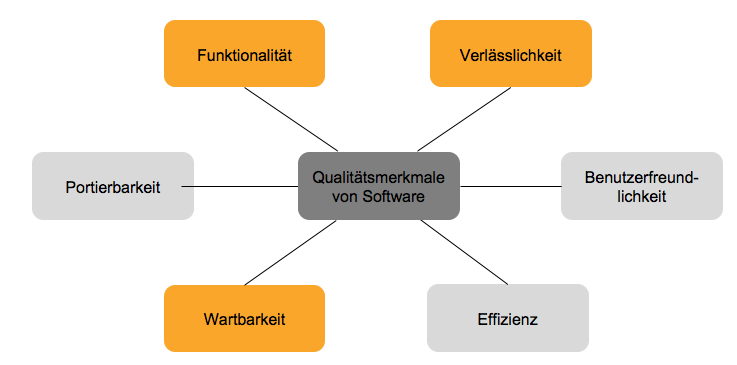
\includegraphics[width=11cm]{Abbildungen/merkmale}
                    \caption[Qualitätsmerkmale von Software]{Qualitätsmerkmale von Software}
                    \label{abb:merkmale}
                \end{center}
        \end{figure}

        \subsection{Funktionalität}

            Funktionalität bewertet den Funktionsumfang der Software. Kunden kaufen Software in der Annahme, dass diese einen Mehrwert für sie darstellt. Das bedeutet, dass die Software die Arbeit des Kunden erleichtert oder die Qualität der Arbeit erhöht. Damit ein Mehrwert geschaffen werden kann, müssen die geforderten Funktionen abgedeckt sein. Eine Software zur Verwaltung von Geschäftspartnern würde keinen Mehrwert liefern, wenn es nicht möglich wäre neue Geschäftspartner anzulegen. Sollte Software für den Kunden jedoch keinen Mehrwert darstellen, gibt es keinen Reiz in diese zu investieren. Eine Software, die die funktionalen Erwartungen des Kunden erfüllt ist somit leichter zu vertreiben.

            Sollte die Software dagegen deutlich mehr Funktionen anbieten als tatsächlich genutzt werden, kann es sein, dass der Anwender von der Funktionalität der Software überfordert ist und die Produktivität somit wieder sinkt. Jede Funktion, die über die Bedürfnisse des Kunden hinausgeht, stellt somit Entwicklungsaufwand dar, der die Kaufbereitschaft des Kunden nicht weiter erhöht, sondern sogar reduzieren kann.

            Für die Entwicklung der Software bedeutet dies, dass die Funktionen, die der Kunde wünscht, implementiert sein sollen, aber keine oder kaum darüber Hinausgehende. Somit wird der Entwicklungsaufwand auf das nötigste reduziert und die Zufriedenheit des Kunden optimiert.
            Um diese Ziele zu erreichen muss die Funktionalität im Rahmen der Softwareentwicklung betrachtet werden und ist somit das erste Bewertungskriterium, dass im weiteren Verlauf dieser Arbeit betrachtet wird.

        \subsection{Verlässlichkeit}

            Durch den bisherigen Einsatz von Mainframes im betrachteten Unternehmen im Bereich der Bausparkasse sind Anwender und Kunden eine hohe Zuverlässigkeit der Software bezüglich der Erreichbarkeit und der Korrektheit der ausgegebenen Ergebnisse gewohnt. Da im Rahmen von Bauspar- und Baufinanzierungsverträgen große Geldbeträge verarbeitet werden, ist es wichtig, dass bei der Verarbeitung eben dieser keine Fehler auftreten. Ein Verlust von Daten, wie Kontoständen oder Personendaten, wäre ebenfalls sehr kritisch, da dies das Vertrauen der Kunden reduziert und diese weniger Produkte nachfragen.

            Die Verfügbarkeit der Software ist im Fall der Bausparkasse jedoch nachrangig, da es sich um langfristig orientierte Geschäfte handelt, die meist keine unmittelbaren Reaktionen erfordern.

            Für die Software ist es im betrachteten Rahmen wichtig, dass keine Fehler produziert werden und keine Daten verloren gehen können, da daraus sehr teure und umständlich zu rekonstruierende Fehler entstehen können. Eine hohe Verlässlichkeit der Software ist damit das zweite betrachtete Bewertungskriterium für die Qualität der Software.

        \subsection{Benutzerfreundlichkeit}

            Benutzerfreundlichkeit wird hauptsächlich durch die Anwendungsoberfläche bestimmt. Die Implementierung von Software ermöglicht es zudem, die Anwendungsoberfläche unabhängig von der Datenhaltung und der Datenverarbeitung zu erstellen. Dies geschieht in einer so genannten 3-Schichten-Architektur\footnote{Siehe Glossar.}. Daher kann die Benutzeroberfläche unabhängig von der zugrunde liegenden Programmlogik implementiert und verändert werden.\footnote{SAP SE (R/3 Architektur).}

            Eine intuitive und einfache Benutzeroberfläche kann die Zufriedenheit und Produktivität der Anwender erhöhen, da diese weniger Fehler machen und somit der Schulungsbedarf geringer ist. Allerdings können die Anwender auch während der Einführungsphase der Software geschult werden, sodass sich hieraus ein Einmalaufwand entwickelt. Eine benutzerfreundliche Oberfläche gibt somit den Anwendern ein besseres Gefühl und verringert Aufwand vorab.

            Die SAP SE setzt bei ihrer Software auf festgelegte Design-Richtlinien, die im Rahmen des Fiori\footnote{Siehe Glossar.} Paradigmas vorgegeben sind. Das Entwicklungsteam der Anwendungslogik hat in diesem Fall nur wenig Einfluss auf die Entwicklung der Benutzeroberfläche. Das Design und die Benutzerfreundlichkeit der Software sind daher bei der Entwicklung der Anwendung nachrangig und werden im Rahmen dieser Arbeit nicht betrachtet.

        \subsection{Effizienz}

            Bauspar- und Baufinanzierungsverträge sind meist langfristig orientiert. Die Kunden informieren sich häufig im Rahmen einer umfassenden Beratung und holen meist Vergleichsangebote ein. Bei den bisher genutzten Mainframes werden die eingegebenen Daten in einer Stapel-Verarbeitung, dem so genannten Batch-Processing, häufig in einem großen Block am Tagesende verarbeitet. Weder die Kunden, noch die Mitarbeiter der Bausparkasse sind somit eine Echtzeitverarbeitung gewöhnt. Eine Optimierung der Antwortzeit durch größeren Ressourceneinsatz oder sehr stark optimierte Software ist daher nicht zwingend erforderlich.

            Eine Minimierung der verwendeten Ressourcen bei einer zeitnahen Antwort ist hingegen wünschenswert. Ein minimierter Ressourcenbedarf bedeutet geringere Hardwarekosten, die zu Beginn der Softwarenutzung entstehen sowie geringere Betriebs- und Wartungskosten während der Softwarelebenszyklus.

            Da der Einsatz von modernen Infrastrukturen im Vergleich zu Mainframes die Kosten der IT-Landschaft reduziert, wird vom Kunden jedoch nicht verlangt, dass ein Fokus auf die Optimierung der Effizienz gelegt wird.

        \subsection{Wartbarkeit}

            Da Unternehmen der Finanzindustrie häufigen Änderungen an regulatorischen Anforderungen und Reportinganforderungen ausgesetzt sind, sollte ihre Software möglichst einfach und günstig anzupassen sein. Das bedeutet, dass der Quellcode auch nach längerer Zeit von Personen nachvollzogen werden muss, die die Software nicht entwickelt haben. Außerdem sollte nach Änderungen leicht sicherzustellen sein, dass keine Fehler hinzugekommen sind und die Software noch wie erwartet reagiert.
            Die Software sollte daher gut dokumentiert, leicht verständlich und konsistent prüfbar sein.

            Hinzu kommt, dass bestehende Systeme, die nicht durch die neu einzuführende Software ersetzt werden, in das System eingebunden werden müssen. Die Software sollte daher die Möglichkeit besitzen, Schnittstellen zu diesen anzubieten.

            Die zu entwickelnde Software soll auf ein dynamisches Marktumfeld reagieren können und dabei Schnittstellen zu umliegenden Systemen bereitstellen und diese mit Daten versorgen oder empfangene Daten verarbeiten. Die Wartbarkeit der Software ist daher keine Eigenschaft, die dem Kunden unmittelbar zu Gute kommt, jedoch unerlässlich ist, um die Software langfristig einsetzen zu können.
            Sie wird daher als drittes Qualitätsmerkmal von Software in dieser Arbeit betrachtet.

        \subsection{Portabilität}

            Die Software soll innerhalb eines festgelegten Rahmens auf einer für sie bereitgestellten Hardware-Infrastruktur arbeiten. Von Seiten des Kunden werden daher an die SAP SE keine Ansprüche zur Verwendung der Software auf verschiedenen Systemen und neben anderen Anwendungen auf der gleichen Infrastruktur gestellt, da für die umliegenden Systeme Hardware bereit steht.

            Da das Unternehmen SAP SE jedoch Standardsoftware und keine Individualsoftware erstellt, ist es für SAP SE bestrebenswert, dass die im Rahmen dieses Projektes entwickelte Software für weitere Kunden anwendbar ist. Da SAP Anwendungen in einer eigenen Laufzeitumgebung auf einem Betriebssystem laufen und dies bereits für andere Anwendungen im SAP Kontext umgesetzt wurde, ist die Kompabilität der Software mit verschiedenen Hardware- und Softwareinfrastrukturen keine Aufgabe der Entwickler für die Geschäftsanwendung.
            Die Portabilität der im SAP Umfeld entwickelten Anwendungen wird somit als gegeben angenommen.

            Im Folgenden werden als Qualitätsmerkmale die Funktionalität, Verlässlichkeit und Wartbarkeit von Software herangezogen. 
    \chapter{Vorgehensmodelle zur Softwareentwicklung}
\label{cha:vorgehensmodelle}

%----------------------------------
%
% Klassische Entwicklungsweise am Beispiel des Wasserfallmodells
%
%----------------------------------
    \section{Klassische Entwicklungsweise am Beispiel des Wasserfallmodells}
    \label{sec:wasserfall}

        In diesem Abschnitt wird das Wasserfallmodell als ein Beispiel für eine klassische Herangehensweise der Softwareentwicklung betrachtet. Das Wasserfallmodel ist ein häufig verwendetes Modell in der Softwareentwicklung. Es bildet die Grundlage zu weiteren Verfahren, wie beispielsweise dem V-Modell, das versucht die Tests der Software deutlich früher einzubinden. Im ersten Teil dieses Abschnitts wird dieses vorgestellt und die einzelnen Phasen erläutert und im zweiten Teil werden die gängigen Kritiken am Wasserfallmodell erklärt.

        Dieser Abschnitt dient dazu einen Vergleichswert zu agilen Methoden zu schaffen und, um die Vor- und Nachteile der klassischen Modelle, mit denen der agilen Entwicklungsmethoden, vergleichbar zu machen.

        \subsection{Vorgehensweise des Wasserfallmodels}

        Das Wasserfallmodel gibt eine Menge von Phasen für die Softwareentwicklung vor, bei der jede Phase vollständig abgeschlossen werden muss, bevor die nächste Phase beginnt.

        \begin{figure}[!htbp]
                \begin{center}
                    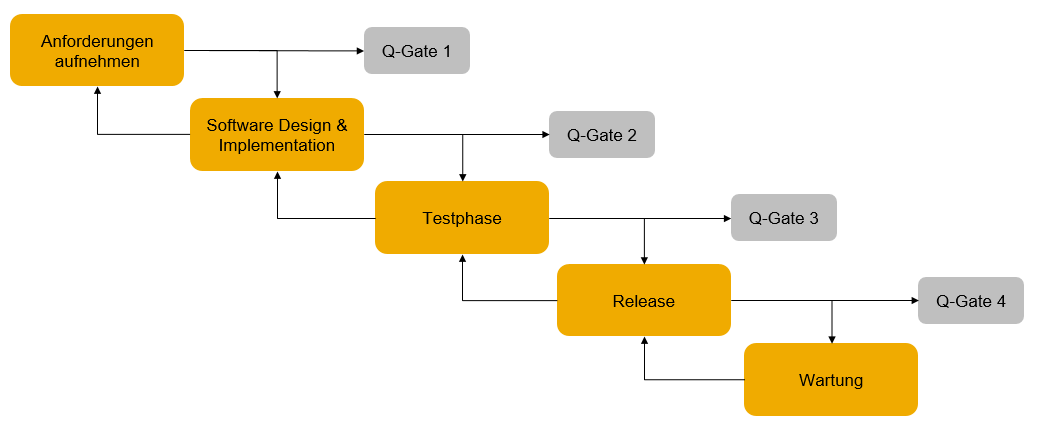
\includegraphics[width=12cm]{Abbildungen/waterfall}
                    \caption[Wasserfallmodell zur Softwareentwicklung]{Wasserfallmodell zur Softwareentwicklung\protect\footnotemark}
                    \label{abb:waterfall}
                \end{center}
        \end{figure}

        \footnotetext{Eigene Abbildung in Anlehnung an Petersen (Waterfall Model).}

        Dies wird in \autoref{abb:waterfall} dargestellt. Die in gold hervorgehobenen Elemente stellen den Hauptprozess einer Variante des Wasserfallmodels dar und die grau markierten Elemente stehen für so genannte \emph{Quality Gates}. Quality Gates stellen häufig eine Checkliste dar, mit deren Hilfe überprüft werden kann, ob alle Schritte der vorhergegangenen Phase absolviert sind.

        In der ersten Phase werden die Anforderungen des Kunden an das Softwareprojekt aufgenommen und formalisiert. Dies umfasst eine umfangreiche Spezifikation, die das Ziel des Projektes konkret vorgibt.\footnote{Vgl. Petersen (Waterfall Model), S.389.}

        Im Anschluss daran wird die Lösung entworfen und implementiert. Dies umfasst eine vollständige Architektur der Software, auf deren Grundlage die Implementation stattfindet. Im Rahmen des Quality Gates wird überprüft, ob in der Design und Implementierungsphase die Anforderungen aus der ersten Phase des Wasserfallmodels erfüllt wurden. Wenn Anforderungen nicht erfüllt sind, muss die Implementierung überprüft werden, oder die Anforderungen müssen überarbeitet werden.\footnote{Vgl. Petersen (Waterfall Model), S.389.}
        Eine Ergänzung des Wasserfallmodels ist die Möglichkeit bei einem neuen Kenntnisstand zu vorherigen Phasen zurückzukehren, um dort nachzubessern.\footnote{Vgl. Royce (Development of large software systems), S.329.}
        Zu diesem Zeitpunkt besteht im Entwicklungsprozess das erste Mal ein lauffähiges Produkt.

        Nach der Implementierung wird die Software erstmals umfangreich getestet. Hierbei sollen alle möglichen Programmabläufe und Konfigurationen geprüft werden.\footnote{Vgl. Petersen (Waterfall Model), S.389.} Eine umfangreichere Betrachtung von Softwaretests folgt in \autoref{cha:einfuehrungQS}.

        Der Release der Software entspricht der Produktivsetzung eben dieser. Ab diesem Moment können Anwender die entwickelte Software verwenden.\footnote{Vgl. Petersen (Waterfall Model), S.390.} Häufig wird der Release mit Schulungen für die Anwender verbunden.

        Den Abschluss bildet die Wartung der Software, falls im Rahmen der produktiven Anwendung weitere Fehler auftauchen.

        \subsection{Probleme und Herausforderungen im Wasserfallmodell}

            Die Testphase der Software im Wasserfallmodell ist für das Projekt häufig sehr kritisch, da sie sehr arbeitsintensiv und zeitaufwändig ist. Werden Fehler gefunden, müssen diese verbessert werden und es entsteht ein iteratives Vorgehen, dass sich abhängig von der Zahl und Komplexität der Fehler sehr lange hinziehen kann.\footnote{Vgl. CTG (Survey of System Development), S.1.}

            Ein weiterer Kritikpunkt am Wasserfallmodell ist, dass erst sehr spät im Projekt eine lauffähige Software entsteht und somit das Projekt zwingend zu Ende geführt werden muss, damit es einen Mehrwert liefern kann.\footnote{Vgl. CTG (Survey of System Development), S.1.}

            Schließlich werden Entscheidungen zu Design, Implementation und Tests sehr früh im Projekt getroffen werden und dies häufig auf einer unzureichenden Faktenbasis.\footnote{Vorwort von Jim Highsmith in Poppendieck (Lean Software Development).} Die Annahmen, die zu Beginn des Projektes getroffen werden lassen sich nur schwer Rückgängig machen, da zu diesen umfangreiche Dokumentationen bestehen, die verändert werden müssen.

%----------------------------------
%
% Prinzipien der agilen Softwareentwicklung
%
%----------------------------------
    \section{Prinzipien der agilen Softwareentwicklung}
    \label{sec:agilePrinzipien}

        \begin{quote}
          \enquote{Achieving a product which satisfies the user's needs normally requires an iterative approach to software development with continual feedback from a user perspective.}\footnote{ISO 9126-1 (Information Technology), S.4.}
        \end{quote}

        Agile Methoden verfolgen das Ziel den Endbenutzer früher in die Softwareentwicklung einzubeziehen, um ein Produkt zu entwerfen, dass tatsächlich benötigt wird. Hierzu werden möglichst schnell und möglichst viele einzelne, aber lauffähige Code-Fragmente entwickelt, die dem Kunden vorgeführt werden um diesen ein Gefühl für die Software zu geben. Das frühe Feedback des Kunden ermöglicht es, bereits während des Entwicklungsprojekts Anpassungen vorzunehmen, um die realen Bedürfnisse zu erfüllen.

        Hierzu existieren Prinzipien, die einfach und granular die Idee der agilen Entwicklung herunterbrechen. Diese werden im agilen Manifest festgehalten und verbreitet.\footnote{Vgl. Beck (Agile Manifesto).}

        \subsection{Individuals and interactions over processes and tools}

            Klassische Softwareentwicklung ist sehr weit standardisiert und geplant. Dadurch sind die Entwickler häufig sehr unflexibel und können nicht auf Wünsche oder Anpassungsvorschläge reagieren, wenn diese den Zeitplan verletzen.\footnote{Vgl. Schneider (Abenteuer Softwarequalität), S.187.}

            Um dieser Entwicklung entgegenzuwirken stellt das agile Manifest die Interaktion mit dem Kunden und den Entwicklern an erste Stelle, anstatt, dass diese von Prozessen regiert werden.

            Insgesammt soll so ein reger Austausch gefördert und auf die Bedürfnisse der einzelnen Personen soll eingegangen werden.\footnote{Vgl. Sutherland, (Agile Softwareentwicklung).}

        \subsection{Working software over comprehensive documentation}

            Durch einen hohen bürokratischen Aufwand und eine umfangreiche Planung der Software wird zu Beginn des Projektes sehr viel Arbeitskraft investiert, ohne, dass diesen ein konkreter Mehrwert gegenüber steht. Durch die dynamische Grundhaltung bei der agilen Entwicklung wird zu Beginn sehr wenig Zeit in die Planung investiert, die Entwicklung wird direkt gestartet und schon nach kurzer Zeit gibt es lauffähige Programmbestandteile.\footnote{Vgl. Sutherland, (Agile Softwareentwicklung).}

            Dieses Prinzip drückt aus, dass der Aufwand der Dokumentation nicht größer sein soll, als der Entwicklungsaufwand. Dem Projektteam soll bewusst sein, dass eine ausführbare Software mehr wert innehat, als eine umfangreiche Planung und Dokumentation einer unfertigen Software.

        \subsection{Customer collaboration over contract negotiation}

            Die SAP SE hat als Hersteller von Standardsoftware zur Unternehmenssteuerung das Ziel Software zu entwickeln und diese zu verkaufen. Der Verkauf von Software wird erheblich erleichtert, wenn diese ein Bedürfnis des Kunden erfüllt und die tägliche Arbeit für diesen erheblich vereinfacht.

            Um die Anforderungen des Kunden zu verstehen und bei der Entwicklung der Software zu berücksichtigen, sollte dieser schon früh einbezogen werden. Die agilen Methoden sollen dabei auf die Wünsche des Kunden reagieren, statt jede Abweichung eines aufgestellten Plans mit umfangreichem bürokratischen Aufwand nachzuverhandeln.\footnote{Vgl. Sutherland, (Agile Softwareentwicklung).}

        \subsection{Responding to change over following a plan}

            Insbesondere bei längeren Projekten ist es meist absurd anzunehmen, dass die Anforderungen des Unternehmens in ferner Zukunft bekannt sind. Bei Unternehmen der Finanzindustrie werden häufig neue regulatorische Anforderungen veröffentlicht oder das Marktumfeld verändert sich. Um auf diese Änderungen auch während der Projektlaufzeit eingehen zu können und keine zum Release veraltete Software einzusetzen sollte im Projekt auf Veränderungen eingegangen werden.\footnote{Vgl. Sutherland, (Agile Softwareentwicklung).}

%----------------------------------
%
% Ausgewählte Methoden der agilen Softwareentwicklung
%
%----------------------------------
    \section{Ausgewählte Methoden der agilen Softwareentwicklung}
    \label{sec:agileMethoden}

        Im Folgenden werden konkrete Herangehensweisen zur agilen Entwicklung vorgestellt. Diese sind genau wie die Prinzipien des agilen Manifests sehr allgemein und flexibel gehalten, um den Entwicklern hinreichend Freiraum zu geben um Ideen ausleben zu können.

        \subsection{Lean Software Development}

            Die Grundlage des Lean Software Developments bildet der Produktentwicklungsprozess von Toyota. Im Anschluss an den zweiten Weltkrieg wurde dort die Automobilproduktion aufgebaut und da in Japan weder der Platz noch die Ressourcen vorhanden waren, um die ineffiziente amerikanische Automobilproduktion zu immitieren, wurden neue Prinzipien in die Entwicklung integriert, die die Lagerhaltung, Massenfertigung und Produktentwicklung betreffen.\footnote{Vgl. Dombrowski (Lean Development), S.7.}

            Die bisherige Annahme im Produktentwicklungsprozess, unabhängig von Software, Autos o.ä., war, dass ein Fehler, der während der Planung eliminiert wird um den Faktor 1000 günstiger ist als ein Fehler, der beim Kunden entdeckt wird. Dies leitet sich aus der so genannten Zehnerregel der Fehlerkosten ab. \autoref{abb:zehnerregel} illustriert die exponentiell wachsenden Fehlerkosten. Ein Fehler, der einen Euro kostet, wenn er während der Planung entdeckt wird, kostet, wenn er beim Kunden entdeckt wird, beispielsweise 1000 Euro. Das Modell der Zehnerregel sagt aus, dass Fehler, die durch eine umfassende Fehlerprävention früh gefunden werden, trotz erhöhter Qualitätssicherungskosten, in der Summe günstiger sind, als Fehler, die erst sehr spät entdeckt und nachträglich ausgebessert werden müssen.\footnote{Vgl. Brüggemann (Grundlagen Qualitätsmanagement), S.29.}

            \begin{figure}[!htbp]
                \begin{center}
                    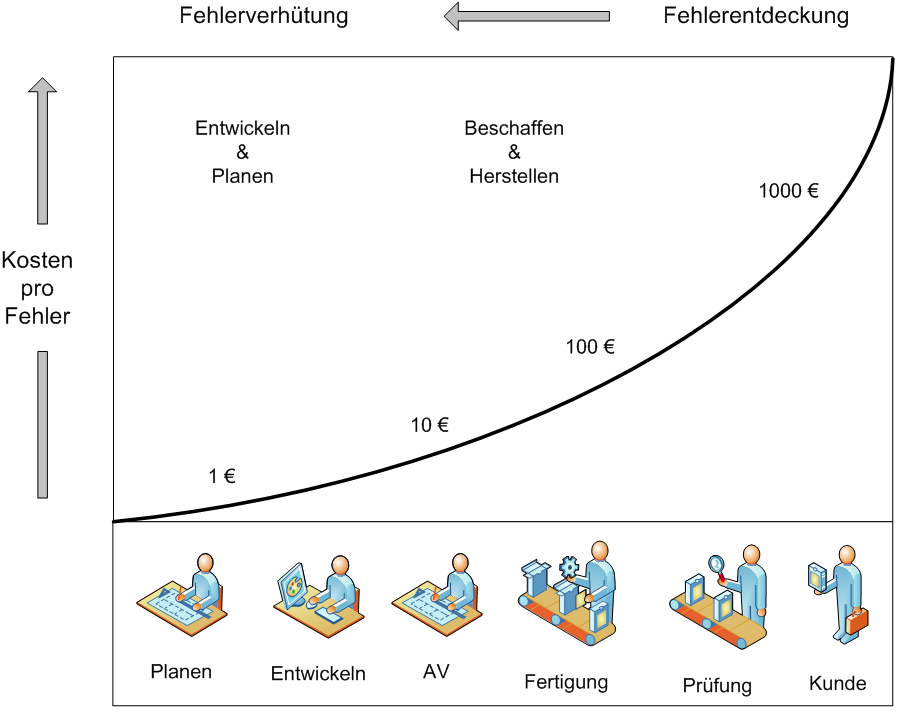
\includegraphics[width=11cm]{Abbildungen/zehnerregel}
                    \caption[Zehnerregel der Fehlerkosten]{Zehnerregel der Fehlerkosten\protect\footnotemark}
                    \label{abb:zehnerregel}
                \end{center}
            \end{figure}

            \footnotetext{Six Sigma Black Belt (Zehnerregel der Fehlerkosten).}

            Im Rahmen von Lean Development halten sich die praktizierenden Unternehmen während des Designprozesses jedoch möglichst viele Optionen offen, um während des Produktionsprozesses Entscheidungen auf einer optimalen Faktenbasis zu treffen und nicht auf Basis plausibler Annahmen.\footnote{Vgl. Poppendieck, 2003, S.5.} Solche Design- und Funktionsentscheidungen werden in agilen Methoden erst sehr spät getroffen, da die Anforderungen des Kunden erst zu Beginn jeder Iteration festgelegt werden und nicht in einem umfangreichen Scopedokument zu Beginn des gesamten Projektes.

             Einige Prinzipien des Lean Developments lassen sich zwar auf klassische Softwareentwicklungsmethoden anwenden, sind aber in einem agilen Umfeld leichter zu praktizieren und implementieren. Der Entwicklungsprozess baut auf sieben Prinzipien auf, die zusammen mit agilen Methoden auch auf die Softwareentwicklung angewendet werden können.\footnote{Vgl. Poppendieck (Lean Software Development), S.13.}:

            \begin{itemize}
                \item Eliminiere Überschuss
                \item Verstärke Lernprozesse
                \item Triff Entschiedungen so spät wie möglich
                \item Liefer Endprodukte so schnell wie möglich
                \item Stärke das Team
                \item Fördere Integrität
                \item Hab eine allumfassende Perspektive
            \end{itemize}

            Im Folgenden wird eine kurze Einführung der Prinzipien gegeben, mit einer Erläuterung, wie sie als agiler Prozess aufzusetzen sind.

            \enquote{Waste is anything that does not add value to a product, value as perceived by the customer.}\footnote{Poppendieck (Lean Software Development), S.13.} Der Überschuss umfasst, bezogen auf die Softwareentwicklung, nicht nur sämtliche Applikationen, die nicht benötigt werden. Vielmehr enthält er auch ungenutzte Funktionen, sowie das Potenzial zu möglichen, zukünftigen Erweiterungen im Programm. Das Ziel sollte es sein, den Umfang des Programms so klein wie möglich zu halten, um die unmittelbaren Bedürfnisse des Kunden zu befriedigen. Das bedeutet, dass in jeder Iteration des Entwicklungsprozesses nur die Funktion entwickelt wird, die der Anwender braucht und die am höchsten priorisiert ist. Rein statistisch werden etwa 50\% aller Funktionen einer Software selten oder nie genutzt.\footnote{Ebert (Software Measurement).} Wenn dieser Überschuss eliminiert wird, werden die Programme schlanker, einfacher und günstiger in der Wartung, ohne das der Anwender auf wichtige Funktionen verzichten muss.

            Die Entwicklung eines Produktes ist im Gegensatz zur Herstellung eines Produktes kein linearer Prozess, der vorher skizziert und abgearbeitet werden kann. Obwohl die Variation in der Produktion reduziert, beziehungsweise eliminiert werden soll, ist sie im Entstehungsprozess eines Produkts durchaus wünschenswert, um die bestmögliche Lösung zu finden.\footnote{Vgl. Ballard (Iteration in design), S. 2f.} Damit möglichst viele Optionen betrachtet werden, und, um sich mit fortgeschrittenem Kenntnisstand für eine zu entscheiden hat Toyota das so genannte \emph{Set-Based Concurrent Engineering} entwickelt. Hierbei werden mehrere Prototypen in die Entwicklung mitgeführt, statt direkt zu Entwicklungsbeginn einen Designstop einzulegen. Diese Protoypen werden mit dem jeweils aktuellen Kenntnisstand weiterentwickelt und eine Entscheidung zu Gunsten einer Variante fällt so spät wie möglich. Zur Entwicklung dieser Methoden wird ein Prozess von drei Oberpunkten vorgesehen, die die Menge von Möglichkeiten filtern:

            \begin{itemize}
                \item \enquote{Map the design space
                \item Integrate by intersection
                \item Establish feasibility before commitment}\footnote{Sobek (Set-Based Concurrent Engineering), S.73.}
            \end{itemize}

            Zunächst wird daher der Rahmen festgelegt, in dem entwickelt werden darf. Dies betrifft, übertragen auf die Softwareentwicklung, Programmiersprachen und Systeme. Im Anschluss werden Konzepte in diesem Rahmen übereinandergelegt und die Variation auf das Nötigste reduziert. Abschließend werden alle verbliebenen Vorgehensweisen auf Machbarkeit geprüft und auf Basis dieses Ergebnisses wird eine Entscheidung getroffen. Bis zur Entscheidung für eine Vorgehensweise lernen die Entwickler aus dem Entwicklungsprozess. Schließlich wird die Möglichkeit, die den größten Nutzen bietet umgesetzt. Dies ist auch der Grund dafür, dass eine möglichst späte Entscheidung angestrebt wird.\footnote{Vgl. Sobek (Set-Based Concurrent Engineering), S.73f.}

            Die Vorgabe so schnell wie möglich Ergebnisse zu liefern bedeutet nicht, dass ein unfertiges oder unreifes Produkt ausgeliefert werden soll, sondern, dass lauffähige Versionen entstehen, auf deren Grundlage die Entwicklung voranschreiten kann. Somit kann ein Kunde herausfinden, was er benötigt und die Richtung des Projektes besser gesteuert werden. Dies führt zu kurzen Iterationen, die lauffähige Ergebnisse liefern.\footnote{Vgl. Poppendieck (Lean Software Development), S.74ff.}

            Die reine Anwendung von Prozessen führt häufig nicht zu den gewünschten Ergebnissen. Vielmehr geht es ebenfalls darum, die Mitarbeiter in den Prozess der Produktentstehung einzubinden und somit alle Ideen und Kompetenzen zu nutzen. Bisherige Softwareentwicklungsprozesse zielen darauf ab, zu Beginn der Entwicklung Entscheidungen von einer Hand voll Personen treffen zu lassen, die die tatsächliche Implementierung meist nicht persönlich umsetzen. In einem Lean Development Umfeld sollen die Entscheidungen von den umsetzenden Personen getroffen werden und die oberen Hierarchien durch Reports, Grafiken und regelmäßige Meetings lediglich informiert werden. Dies beschleunigt Iterationen und ermöglicht mehr Tests und Versuche, die zu besseren Ergebnissen führen.\footnote{Vgl. Poppendieck (Lean Software Development), S.98ff.}

            Die Integrität einer Software wird daran gemessen, wie zufrieden jemand ist, der mit dieser Software arbeitet, unabhängig davon, ob eben dieser Anwender oder Entwickler ist. Hierbei beruft sich Poppendieck auf die Qualitätskriterien von Software der ISO 9126-1, die oben vorgestellt werden. Sie sagt, dass diese Kriterien nicht durch Prozesse und Messungen umsetzbar sei, sondern durch weise Führung, fachliche Expertise, effiziente Kommunikation und gesunde Disziplin.\footnote{Vgl. Poppendieck (Lean Software Development), S.123ff.} Der Weg zur Integrität einer Software basiert daher auch auf einigen Prinzipien des agilen Manifests.

            Zuletzt soll das Gesamtziel des Projektes nicht aus den Augen verloren werden. Die absolute Optimierung eines Teilbereichs zu Lasten des Gesamtprojekts sollte zwingend vermieden werden.\footnote{Vgl. Poppendieck (Lean Software Development), S.146f.}

            Zusammenfassend ist Lean Software Development eine Menge von Prinzipien, die aus der Entwicklung von Autos abgeleitet wurde und zu Beginn eines Projektes als konkrete Pläne umgesetzt werden sollen. Wie die im Folgenden vorgestellten agilen Programme weißt es auf typische Fehler hin und gibt Ratschläge, wie sie vermieden werden können, ohne hierbei die Freiheit des Teams einzuschränken.

        \subsection{Extreme Programming}

            \begin{quote}
                \enquote{XP is a style of software development focusing on excellent application of programming techniques, clear communication, and teamwork which allows us to accomplish things we previously could not even imagine.}\footnote{Andres (Extreme Programming).}
            \end{quote}

            Extreme Programming räumt mit einigen Konventionen der Softwareentwicklung auf, indem es die bisher bestehenden Prozesse bewusst kritisiert und eigene Werte und Modelle präsentiert, die die Softwareentwicklung vereinfachen. Es legt einen Prozess fest, der die Kommunikation und Kollaboration im Team fördert und Prozessteile der Softwareentwicklung überspitzt anwendet. So werden beispielsweise die Tests nicht im nachhinein durchgeführt, sondern vor der Entwicklung der Software entwickelt und automatisiert, sodass nach jeder Veränderung der Software die korrekte Funktionalität überprüft werden kann.

            \begin{figure}[H]%[!htbp]
                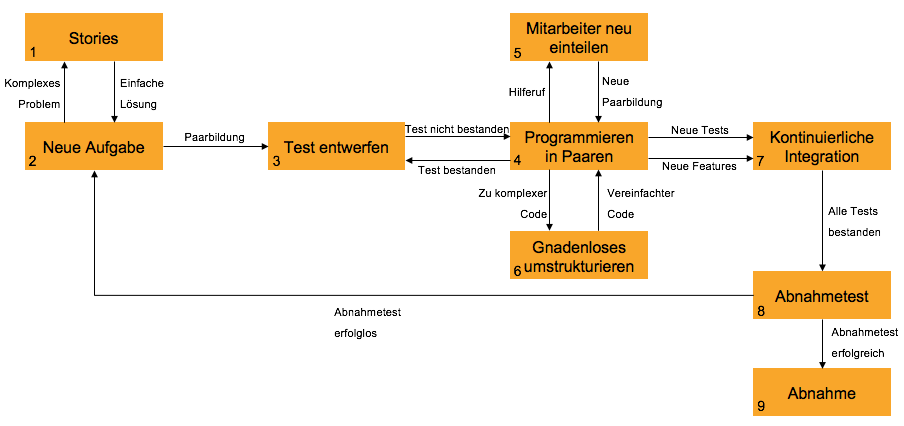
\includegraphics[width=15cm]{Abbildungen/XP_vorgehensmodell}
                \caption[Vorgehensmodell des Extreme Programming]{Vorgehensmodell des Extreme Programming\protect\footnotemark}
                \label{abb:xpmodel}
            \end{figure}

            \footnotetext{Eigene Abbildung in Anlehnung an Uni Saarland (Extreme Programming).}

            \autoref{abb:xpmodel} zeigt das Vorgehensmodell des Extreme Programming, dessen Bestandteile im Anschluss genauer erläutert werden. Das Vorgehen beginnt mit einer neuen Aufgabe (Element 2 der Abbildung), die in das Team übergeben wird und durch User Stories vereinfacht wird, bis sie in den Kreislauf übergeben werden kann. Nach der Fertigstellung einer Aufgabe wird mit einer neuen Aufgabe begonnen, bis alle Aufgaben des Programms abgenommen wurden.

            Extreme Programming orientiert sich dennoch an einem groben Prozess zur Entwicklung von Software. Zunächst wird eine User Story entworfen (Element 1), das heißt ein Anwender beschreibt was er tun muss und an welchen Stellen er dabei unterstützt werden muss.\footnote{Vgl. Uni Saarland (Extreme Programming).} Zur Erläuterung des Prozesses wird nachfolgend beispielhaft das Anlegen eines Vertrags in einer Filiale aus Sicht eines Angestellten betrachtet.

            Der Anwender möchte die Daten des Kunden in die Softwareoberfläche eintragen und anschließend einen Vertrag mit den Konditionen für diesen Kunden ausdrucken. Die Daten sollen zudem in der Datenbank der Bausparkasse hinterlegt werden. Daraus ergibt sich eine neue Aufgabe für die Softwareentwickler.

            Extreme Programming sieht vor, dass für jede zu entwickelnde Komponente zunächst ein Test (Element 3) geschrieben wird. Die Tests bilden das Pendant zur klassischen Spezifikation und werden nach jeder Änderung der Software überprüft, um so eine ständige Lauffähigkeit des Moduls zu gewährleisten. Ein Test würde beispielsweise prüfen, wie mit unvollständigen Angaben umgegangen wird oder wie verfahren wird, wenn kein Drucker erreichbar ist. Bei der Erstellung der Test-Fälle sollen alle gewöhnlichen Eingaben, ungültige Eingaben und Randwerte geprüft werden.\footnote{Vgl. Wells (Unit Tests).}

            Auf Grundlage der entworfenen Tests startet die Entwicklung, die die Ansprüche des Anwenders, die im Test formalisiert wurden, erfüllen soll. Im Gegensatz zur klassischen Entwicklung von Software, bei der jeder Entwickler für einen Baustein des Programms zuständig ist und diesen in Einzelarbeit vorantreibt, wird im Extreme Programming Pairprogramming empfohlen (Element 4). Dies bedeutet, dass zwei Programmierer zur gleichen Zeit am selben Computer arbeiten und eine Person tippt, während die andere Person die Entwicklung kontrolliert. Außerdem sollen alle Entwickler jederzeit den gesamten Code kennen und dürfen an jeder Stelle etwas verändern, sobald sie Fehler entdecken. Das Ziel ist es die Abhängigkeit von einzelnen Entwicklern zu reduzieren und schon während der Entwicklung eine ständige Kontrolle durch den Partner zu haben. Studien haben außerdem nachgewiesen, dass zwei Entwickler die Entwicklungszeit reduzieren und weniger Fehler produzieren.\footnote{Williams (Pair-Programming), S.5f.}

            Extreme Programming hat darüber hinaus noch zwei Prinzipien, die bei der klassischen Softwareentwicklung in dieser Form nicht angewendet werden. Zunächst wird immer nur ein aktuelles Problem gelöst und es werden keine Pläne für zukünftige Integrationen und Erweiterungen im Code umgesetzt. Der Code soll so einfach wie möglich gehalten werden. Die Idee dahinter ist, dass ein einfacher Code besser anzupassen ist, als komplizierter Code mit einer Schnittstelle, die eventuell nie gebraucht wird.\footnote{Rumpe (Extreme Programming), S.3.}

            Das zweite Prinzip ist der selbstdokumentierende Code. Über sprechende Methodennamen und Kommentare soll jeder Entwickler zu jeder Zeit verstehen, was sich der Autor des Codes gedacht hat. Sprechender Code soll die Dokumentation der Software obsolet machen. Dies geschieht aus dem Grund, dass Dokumentationen häufig nicht aktuell sind oder nicht mit dem gleichen Eifer wie der Code entwickelt werden und somit fachlich falsch sind. Diese Ziele werden erreicht, indem sehr viele Kommentare verwendet werden und das bisher entwickelte \emph{Refactored} wird. Das bedeutet, dass Codebruchstücke, wie beispielsweise eine Tabellenabfrage in eine Methode ausgegliedert werden und stattdessen die Methode im Hauptprogramm aufgerufen wird. Diese ständigen Restrukturierungen vereinfachen das bisher Entwickelte und lassen den Umfang des Programms nicht ausufern.\footnote{Rumpe (Extreme Programming), S.6f.}

            Die entwickelten Bausteine werden meist täglich in die bestehende Software integriert und fortlaufend getestet (Element 7 und 8). Am Ende des agilen Projektes steht die Abnahme (Element 9) durch den Kunden.

            Natürlich stößt auch das Extreme Programming in Projekten an seine Grenzen. Die Pairprogramming Methodiken setzen voraus, dass die Entwickler auf engem Raum zusammenarbeiten, da Pair-Programming Aktivitäten sonst erschwert werden. Außerdem sollte für die häufige Abstimmung und Kommunikation das Team sehr klein gehalten werden, meist werden 9-12 Personen empfohlen.\footnote{Vgl. Uni Saarland (Extreme Programming).}

            Extreme Programming stellt konkrete Anforderungen an das Team und lässt in der Umsetzung die wenigsten Freiheiten der agilen Methoden. Es ist, wie der Name impliziert, eine sehr extreme Herangehensweise, die Tests, Entwicklung und Flexibilität maximiert. Es können jedoch vereinzelte Methoden des Extreme Programming in anderen agilen Verfahren verwendet werden, um einen Teil der methodischen Flexibilität zu erhalten.

        \subsection{Scrum}
        \label{subsec:scrum}

            Scrum ist ein \enquote{Ein Rahmenwerk, innerhalb dessen Menschen komplexe adaptive Aufgabenstellungen angehen können, und durch das sie in die Lage versetzt werden, produktiv und kreativ Produkte mit dem höchstmöglichen Wert auszuliefern.}\footnote{Schwaber (Scrum Guide), S.3.} Es ist
            \begin{itemize}
                \item \enquote{Leichtgewichtig
                \item Einfach zu verstehen
                \item Schwierig zu meistern.}\footnote{Schwaber (Scrum Guide), S.3.}
            \end{itemize}

            Im Gegensatz zum Extreme Programming ist Scrum ein Rahmenwerk statt einer Methode, das neben konkreten Managementvorgaben sehr viel Gestaltungsfreiraum bietet. Scrum setzt auf einen iterativen, inkrementellen Ansatz. Das bedeutet, dass kurze Phasen der Entwicklung ständig wiederholt werden und das Endprodukt Stück für Stück aufgebaut wird. Mit jeder abgeschlossenen Phase wird die Software um einen weiteren Baustein ergänzt.

            Für Scrum-Teams wird eine Personenanzahl von 5-9 Entwicklern zuzüglich Scrum Master und Product Owner empfohlen. Somit soll die Organisation flexibel genug sein, um sich selbst koordinieren zu können, aber groß genug um alle notwendigen Kenntnisse abzudecken, sodass das Team während der Softwareentwicklung nicht auf externe Hilfe angewiesen ist.\footnote{Vgl. Schwaber (Scrum Guide), S.6.} In \autoref{tbl:scrumrollen} werden die Rollen im Scrum-Team zusammengefasst und im Anschluss werden diese erklärt.

            \begin{table}[!htbp]
            \begin{tabularx}{\textwidth}{|l|c|X|}
                \hline
                Name & Anzahl & Aufgaben \\
                \hline
                Product Owner & 1 & Kommunkation mit Kunden \\
                && Verwalten des Product Backlog \\
                && Verantwortung zum Erfolg des Projektes \\
                &&\\
                Scrum Master & 1 & Vermittler zwischen Product Owner und Team \\
                && Erfahrener Ansprechpartner für Fragen zu Scrum \\
                && \\
                Entwickler & 5-9 & Entwicklung der Inkremente \\
                && Einschätzung zu Aufwänden für Sprints \\
                \hline
            \end{tabularx}
            \caption{Rollen im Scrum-Team}
            \label{tbl:scrumrollen}
            \end{table}

            Der Product Owner hat die Verantwortung, dass der Kunde das erhält, was er sich wünscht. Er steht in ständigem Austausch mit diesem, präsentiert Zwischenergebnisse und trägt die neuen Wünsche priorisiert in das Entwicklungsteam. Alle Wünsche und Anforderungen, die an das Team gestellt werden, haben über den Product Owner zu laufen.\footnote{Vgl. Maximini (Scrum), S.167f.}

            Der Scrum Master vertritt die Interessen der Entwickler gegenüber Außenstehenden und dem Product Owner. Er sorgt dafür, dass die Scrum-Regeln eingehalten werden und die Entwickler während ihrer Entwicklungsphasen nicht gestört werden. Der Scrum Master verfügt über keine Weisungsbefugnis, sondern versucht einem Ombudsmann ähnlich Win-Win Situationen für alle Parteien zu erreichen. Als erfahrenes Scrum-Teammitglied steht er außerdem für alle Fragen zur Verfügung und schult seine Kollegen bei Bedarf.\footnote{Vgl. Maximini (Scrum), S.170f.}

            Das Entwicklungsteam setzt sich aus einer Vielzahl von Experten zusammen, die alle benötigten Kompetenzen abdecken. Das gesamte Entwicklungsteam ist verantwortlich für den kompletten Code und organisiert sich vollständig selber.\footnote{Vgl. Schwaber (Scrum Guide), S.5f.}

            Neben dem Team umfasst Scrum auch Vorgaben zum Ablauf. Hierfür werden eine Menge von Meetings und Phasen vorgegeben, die einen festen Zeitraum haben, der nicht überschritten werden darf. Auf Grundlage dieser Annahmen sind Scrum-Projekte sehr planbar.

            \enquote{Das Herz von Scrum ist der Sprint, eine Time Box von maximal einem Monat, innerhalb dessen ein fertiges (\emph{Done}), nutzbares und potenziell auslieferbares Produkt-Inkrement hergestellt wird}\footnote{Vgl. Schwaber (Scrum Guide), S.8.}. Dies entspricht der oben bereits vorgestellten Entstehung von Software durch Bausteine, die ein Grundkonstrukt, um Funktionen erweitern. Wichtig ist dabei, dass jeder Baustein fertig ist, was durch den Ausdruck Done im obigen Zitat versinnbildlicht wird. Die Definition of Done muss von Product Owner, Scrum-Team und Kunde vorab festgelegt und festgehalten werden, damit es dort zu keinen Missverständnissen kommt.

            Ein Sprint dauert für gewöhnlich vier Wochen und beinhaltet eine Menge von Ereignissen:
            \begin{itemize}
                \item Sprint Planning
                \item Daily Scrums
                \item Sprint Review
                \item Sprint Retrospektive
            \end{itemize}

            \begin{figure}[!htbp]
                \begin{center}
                    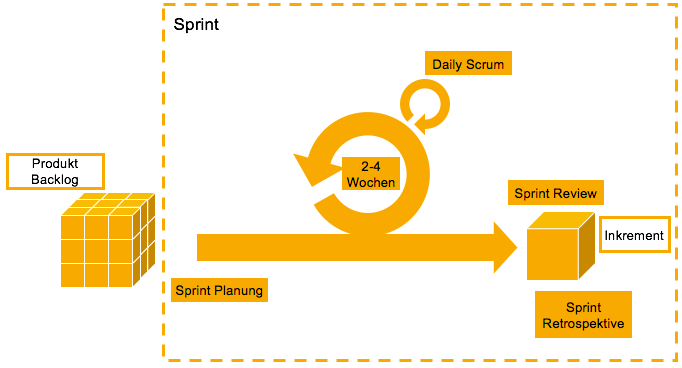
\includegraphics[width=\textwidth]{Abbildungen/scrum}
                    \caption[Planungszyklus Scrum]{Planungszyklus Scrum}
                    \label{abb:scrum}
                \end{center}
            \end{figure}

            \autoref{abb:scrum} illustriert den gesamten Scrum-Ablauf. Alle Einträge des Product-Backlogs werden priorisiert in das Scrum-Team getragen und beim Sprint-Planning werden die die Elemente des Product-Backlogs festgelegt, die in diesem Sprint erledigt werden sollen. Daraus entsteht der Sprint-Backlog. Diese Aufgaben sollen in Phasen von zwei bis vier Wochen abgearbeitet werden. Während des Sprints finden tägliche Meetings statt, die Daily Scrums, die in der Abbildung auf dem Sprintzyklus aufsetzen. Diese klären den Status des Sprints und fördern die Kommunikation im Team. Am Ende des Zyklus steht ein Produktbaustein, das so genannte Inkrement, dass die Software ergänzt und erweitert. Nach dem formalen Abschluss durch Retrospektive und Review wird der Zyklus ausgehend vom Product-Backlog neu begonnen.

            Während des Sprints werden keine weiteren Themen zum Scope ergänzt und weder Zeit- noch Qualitätsplanung angepasst. Erst die Sprint-Planung am Ende jedes Zyklus bietet die Möglichkeit zur Nachkalibrierung. Die Dauer eines Sprints ist daher so gewählt, dass das Projekt flexibel genug ist, um auf Anforderungen einzugehen, aber die Entwickler die Chance erhalten sich voll und ganz auf eine Aufgabe zu konzentrieren und nicht ständig durch Anforderungsänderungen aus ihrem Fokus gerissen werden.\footnote{Maximini (Scrum), S.181f.} Im Folgenden werden die vier Phasen eines Sprints weiter aufgeschlüsselt:

            Das \emph{Sprint Planning} dient als Vorbereitung für den kommenden Sprint. Im Zentrum des Planungsprozesses stehen zwei Fragen, die am Ende des Meetings beantwortet sein sollen.
            \begin{itemize}
                \item Was kann in diesem Sprint fertiggestellt werden?
                \item Wie wird die ausgewählte Arbeit erledigt?
            \end{itemize}

            In der ersten Phase präsentiert der Product Owner die Wünsche des Kunden und priorisiert alle Dinge, die bis zum Ende des Sprints geschafft werden sollen. Das Entwicklungsteam diskutiert mit ihm daraufhin, ob die Zeitplanung und Deadlines realistisch sind. Haben sich Product Owner und Scrum Team auf einen Scope geeinigt, kommt es zu Phase zwei des Sprint Planning, in der geplant wird, wie das Sprint-Ziel zu erreichen ist.\footnote{Vgl. Maximini (Scrum), S.182f.}

            Die Vorgehensweise basiert bei Software grob auf der Codestruktur der Methoden, Eigenschaften von Klassen usw. Sie lässt sich beispielsweise durch \emph{Unified Modelling Language} (UML) Klassendiagramme sehr gut erfassen. Hierbei sollen unabhängig von Kompetenzen und Erfahrungen alle Ideen des Teams eingebracht werden. Ein großes Problem bei Sprint Plannings sind häufig Externe, insbesondere Vorgesetzte, die bei jungen Entwicklerteams oft Ratschläge geben, die aber als Weisung aufgenommen werden. Durch die Präsenz weisungsbefugter Personen wird die Kreativität im Team so häufig untergraben und nicht vollkommen ausgeschöpft.
            Der Scrum Master hat zusätzlich noch die Aufgabe sehr dominante und aktive Personen zu bremsen und auch die ruhigeren Charaktere in die Diskussion mit einzubinden. Während des Sprint Plannings und auch dem gesamten Sprint fungiert er als Moderator.\footnote{Vgl. Maximini (Scrum), S.182f.}

            Das \emph{Daily Scrum} findet täglich statt, dauert meist 15 Minuten und ist ein Meeting mit dem gesamten Team. Um Dynamik zu erzeugen und nicht zu überziehen findet es meist im Stehen, kurz vor der Mittagspause, statt. Das Daily Scrum dient dazu, dem gesamten Entwicklungsteam eine Übersicht zu geben, wer wo steht und wie weit man als Team bei der Verwirklichung des Sprint Ziels ist. Außerdem findet man häufiger eine Lösung, wenn Probleme auftreten und diese im Team vorgestellt werden. Jedes Mitglied des Scrum-Teams ist nacheinander an der Reihe und beantwortet in der großen Runde folgende drei Fragen:

            \begin{itemize}
                \item Was habe ich gestern getan?
                \item Was werde ich bis morgen tun?
                \item Wo bin ich dabei auf Hindernisse gestoßen?
            \end{itemize}

            Insbesondere bei der letzten Frage geht es nicht darum Lösungen während des Daily Scrums zu finden, sondern im Scrum das Problem vorzustellen und jemanden zu finden, der es im Anschluss gemeinsam mit angeht. Somit schweift das Team gedanklich nicht ab, wenn es technischer wird. Dem Daily Scrum kommt somit eine Planungs- und Kontrollfunktion zu \footnote{Vgl. Maximini (Scrum), S.183.}.

            Der \emph{Sprint Review} schließt sich an einen Sprint an, um auf Grundlage der Ergebnisse erneut zu planen. Beim Sprint Review sind neben dem gesamten Scrum-Team auch Stakeholder anwesend, denen das Produkt vorgestellt werden soll. Dabei ist wünschenswert, dass die Stakeholder das Produkt selber testen können und die Entwickler dabei die Wünsche und Gedanken der Stakeholder zum Produkt notieren. Auf Grundlage dieses Feedbacks wird anschließend das Produkt kontrolliert und, falls nötig, der Backlog erweitert.\footnote{Vgl. Maximini (Scrum), S.183.}

            Auf Grundlage der Definition of Done werden im Sprint Review die Backlogeinträge abgehakt, die erfüllt sind und die bestehenden Einträge auf Zeit und Erreichbarkeit überprüft. Das Sprint Review stellt somit die Grundlage zum kommenden Sprint Planning dar.\footnote{Vgl. Schwaber (Scrum Guide), S.16.}

            Die \emph{Sprint Retrospektive} stellt das Pendant zum Sprint Planning dar und schließt einen Sprint formell ab. Während beim Sprint Review das erstellte Produkt im Mittelpunkt steht, betrachtet die Sprint Retrospektive die Zusammenarbeit des Scrum Teams und dessen Arbeitsweise. Das Ziel dieses Meetings ist es, Maßnahmen herauszuarbeiten, die die Zusammenarbeit im Team verbessern oder die die Qualität der Endprodukte verbessern. Am Ende des Meetings soll eine Liste mit wenigen, aber greifbaren Maßnahmen stehen, die jedes Teammitglied bis zum Ende des folgenden Sprints umsetzen kann.\footnote{Vgl. Schwaber (Scrum Guide), S.13.}

            Scrum ist eines der bekanntesten agilen Verfahren und wird häufig als Synonym für eine agile Vorgehensweise genutzt. Es gibt Vorgaben zum Management von Anforderungen und lässt dem Entwicklerteam freien Spielraum zur Umsetzung eben dieser. Scrum-Teams bemühen sich, aus jedem Sprint etwas zu lernen und ihre Vorgehensweise im nächsten Sprint anzupassen, um sich kontinuierlich zu verbessern. 
    \chapter{Einführung in die Qualitätssicherung}
\label{cha:einfuehrungQS}

    Um das Ziel der Qualitätssicherung zu verstehen, wird die Qualitätssicherung zunächst vom Qualitätsmanagement abgegrenzt. Das Qualitätsmanagement stellt alle Maßnahmen zur Führung und Steuerung der Qualität im Unternehmen dar, während die Qualitätssicherung \enquote{als Bestandteil des Qualitätsmanagements alle organisatorischen und technischen Maßnahmen, die vorbereitend, begleitend und prüfend der Schaffung und Erhaltung einer definierten Qualität eines Produkts oder einer Dienstleistung dienen.}\footnote{Springer (Qualitätssicherung).} Dabei geht es nicht darum, ein Produkt kontinuierlich zu verbessern, sondern ein vorgegebenes Niveau zu erreichen oder zu halten.

    \begin{quote}
        \enquote{Die Darlegung des Qualitätsmanagements, d.h. alle Tätigkeiten zur Schaffung von Vertrauen, dass die Qualitätsanforderungen erfüllt werden, wird Qualitätssicherung genannt. Als zentrale Maßnahmen braucht es regelmäßige Überprüfungen, ob das Qualitätsmanagementsystem wie geplant funktionert und ob die vorgesehenen Qualitätsmaßnahmen wirklich durchgeführt werden. Solche Überprüfungen heißen Audits.}\footnote{Glinz (Software Engineering), S.120.}
    \end{quote}

    Im Projekt unterscheidet man außerdem zwischen organisatorischen, analytischen und konstruktiven Maßnahmen zur Sicherung der Qualität. Diese werden im Folgenden definiert:

    \begin{description}
        \item[Organisatorische Maßnahmen] Definiert die Aufbau- und Ablauforganisation , die die Softwarequalität im Projekt verankert. Dies schafft die Voraussetzung dafür, dass analytische und konstruktive Maßnahmen durchführbar und wirksam sind.\footnote{Vgl. Schneider (Abenteuer Softwarequalität), S.177.}
        \item[Analytische Qualitätssicherung] In analytischen Verfahren wird ein bereits fertiger Prüfling untersucht, um Fehler zu finden. Analytische Maßnahmen wirken sich auf die Softwarequalität indirekt aus, wenn nämlich die gefundenen Fehler beseitigt werden. Die analytische Qualitätssicherung umfasst das Testen der Software.\footnote{Vgl. Schneider (Abenteuer Softwarequalität), S.177.}
        \item[Konstruktive Qualitätssicherung] Maßnahmen, die bereits bei der Konstruktion von Software auf die Verbesserung ausgewählter Qualitätsaspekte abzielen und nicht erst nachträglich durch Prüfung und Korrektur. Konstruktive Maßnahmen können daher häufig verwendete Standards und Rahmenwerke sein. Darunter fallen auch Qualitätsmanagementsysteme und -modelle wie die ISO 9000 oder Six Sigma.\footnote{Vgl. Schneider (Abenteuer Softwarequalität), S.177.}
    \end{description}

%----------------------------------
%
% Organisatorische Qualitätssicherungsmaßnahmen
%
%----------------------------------
    \section{Organisatorische Qualitätssicherungsmaßnahmen}

        Qualität im Projekt muss an drei Stellen umgesetzt werden und zwar in der Aufbauorganisation, der Ablauforganisation und in Form eines Qualitätsmanagementsystems.

        \subsection{Aufbauorganisation}

            Die Aufbauorganisation bezieht sich dabei auf die Ansiedlung der Qualitätssicherung im Organisationsdiagramm des Unternehmens. Bei einer klassischen, hierarchieschen Struktur ist es zwingend erforderlich, dass die Qualitätsbeauftragten auf allen Hierarchieebenen vertreten sind, ohne, dass die normalen Projektteilnehmer eine Weisungsbefugnis gegenüber diesen haben.\footnote{Vgl. Schneider (Abenteuer Softwarequalität), S.12f.}

            \begin{figure}[!htbp]
                \begin{center}
                    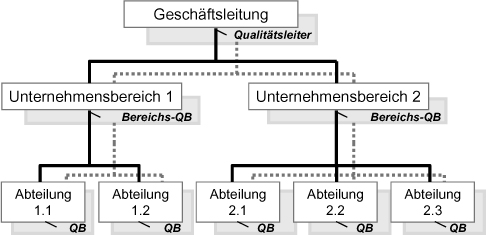
\includegraphics[width=11cm]{Abbildungen/aufbauqs}
                    \caption[Aufbauorganisation mit Qualitätsbeauftragten]{Aufbauorganisation mit Qualitätsbeauftragten\protect\footnotemark}
                    \label{abb:aufbauqs}
                \end{center}
            \end{figure}

            \footnotetext{Schneider (Abenteuer Softwarequalität), S.13.}

            \autoref{abb:aufbauqs} stellt die Soll-Hierarchie in einem Unternehmen dar, dass die Qualitätssicherung in den Fokus stellt. Die \emph{Qualitätsbeauftragten} (QB) sind jeweils auf einer Hierarchiebene mit den Leitern ihrer jeweiligen Abteilungen und empfangen weder von ihren Kollegen, noch von deren Vorgesetzten Weisungen. Sie sind nur gegenüber höher gestellten Qualitätsbeauftragten rechenschaftspflichtig.\footnote{Vgl. Schneider (Abenteuer Softwarequalität), S.13f.}

            Das Qualitätsteam bekommt \enquote{Narrenfreiheit}, was ihnen erlaubt offen Kritik zu üben, ohne Konsequenzen fürchten zu müssen. Diese sollte allerdings gerechtfertigt sein, sodass die negative Konnotation, dass die Narrenfreiheit \enquote{Dümmlichkeit} impliziert, entfällt.\footnote{Expertengespräch mit R. Bihler, SAP SE.}

            Mit Hilfe dieser Struktur wird verhindert, dass Qualitätsverantwortliche durch Druck ihrer Vorgesetzten die eigenen Ansprüche herunterschrauben, da ansonsten Deadlines oder Budgetziele des Projekts nicht haltbar wären.\footnote{Vgl. Schneider (Abenteuer Softwarequalität), S.13.}

        \subsection{Ablauforganisation}

            \begin{quote}
                \enquote{Innerhalb der Ablauforganisation muss das Qualitätsmanagementsystem für alle Abläufe die qualitätsrelevanten Kompetenzen, Verantwortlichkeiten und gegenseitigen Beziehungen festlegen. Man ist dabei bestrebt, möglichst wenig Qualitätsaufgaben separat zu regeln, sondern diese weitestgehend in die Prozesse des Unternehmens zu integrieren.}\footnote{Glinz (Software Engineering), S.119.}
            \end{quote}

            \begin{figure}[!htbp]
                \begin{center}
                    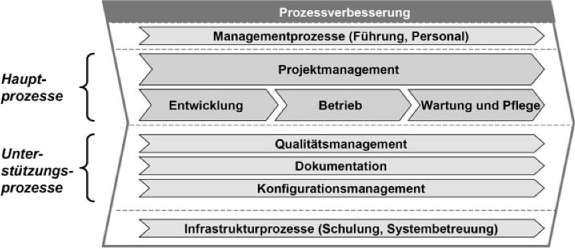
\includegraphics[width=11cm]{Abbildungen/ablaufqs}
                    \caption[Qualitätsmanagement als Unterstützungsprozess]{Qualitätsmanagement als Unterstützungsprozess\protect\footnotemark}
                    \label{abb:ablaufqs}
                \end{center}
            \end{figure}

            \footnotetext{Schneider (Abenteuer Softwarequalität), S.14.}

            \autoref{abb:ablaufqs} zeigt, dass der Qualitätsprozess nicht einsam und für sich stehen soll, sondern eine enge Verwebung mit den bestehenden Prozessen des Unternehmens angestrebt wird. Die Qualitätsprozesse sind unterstützend zum Entwicklungsprozess der Software, da mit qualitativer Software und nicht mit qualitativen Softwareentstehungsprozessen Geld verdient werden kann. Der Qualitätsprozess dient somit zur Unterstützung der Projektprozesse.

        \subsection{Qualitätsmanagementsystem}

            Das Qualitätsmanagementsystem sind nach ISO 8402 alle
            \begin{quote}
                zur Verwirklichung des Qualitätsmanagements erfoderliche Organisationsstruktur, Verfahren, Prozesse und Mittel.\footnote{Schneider (Abenteuer Softwarequalität), S.15.}
            \end{quote}
            Dies steht in direkter Verbindung mit der ISO 8402 Definition des Qualitätsmanagements:
            \begin{quote}
                Alle Tätigkeiten der Gesamtführungsaufgabe, welche die Qualitätspolitik, Ziele und Verantwortlichkeiten festlegen sowie diese durch Mittel wie Qualitätsplanung, -lenkung, -sicherung und -verbesserung im Rahmen des Qualitätsmanagementsystems verwirklichen.\footnote{Schneider (Abenteuer Softwarequalität), S.15.}
            \end{quote}

            Zusammenfassend ist Ziel des Qualitätsmanagementsystems eine Verbesserung des gesamten Unternehmens auf der Prozess bzw. Produktebene. Auf Software angewandt bedeutet dies, dass das Qualitätsmanagementsystem sicherstellt, dass die Software alle internen und externen Ansprüche erfüllt. Dabei ist Qualität kein Selbstzweck, sondern dient stets der Verbesserung des Produkts.

%----------------------------------
%
% Analytische Qualitätssicherungsmaßnahmen
%
%----------------------------------
    \section{Analytische Qualitätssischerungsmaßnahmen}
    \label{subsec:analytischeqs}

        Analytische Qualitätssicherungsmaßnahmen beziehen sich auf Schritte, die nach der Entwicklung einer Software darauf abzielen, die korrekte Funktion eben dieser sicherzustellen. Das bedeutet insbesondere, dass neben einer aktuellen Dokumentation eine Menge von Tests durchgeführt werden müssen, die überprüfen, ob die Software auf Eingaben mit den erwarteten Ausgaben reagiert. Die Länge der Testphase, die sich an die Entwicklung anschließt, kann oft nicht korrekt festgelegt werden, da nicht abzusehen ist, wie viel Code korrigiert werden muss und wie schwerwiegend die Fehler sind. Somit gefährdet die Testphase meist die vorher festgelegte Projektlaufzeit und das Projektbudget.\footnote{Schneider (Abenteuer Softwarequalität), S.83ff.}

        Obwohl die Testphase häufig unerwünscht ist, ist sie essentiell, da Fehler, die noch während des Projekts entdeckt werden, günstiger zu beheben sind, als im späteren Verlauf. Je nach Einsatzgebiet der Software kann ein Fehler der Software die Kosten des Testvorgangs weit übersteigen. Aufgrund dessen sollte jedes Teilprodukt einer Software so früh wie möglich geprüft werden.\footnote{Prechelt (Vorlesung Softwaretechnik), S.6.}

        Ein Test ist nach IEEE Standard 610.12 definiert als:
        \begin{itemize}
            \item \enquote{The process of operating a system or component under specified conditions, observing or recording the results, and making an evaluation of some aspect of the system or component.}
            \item \enquote{The process of analyzing a software item to detect the differences between existing and required conditions (that is, bugs) and to evaluate the features of the software items.}\footnote{IEEE 610.12 (Standard Glossary), S.20.}
        \end{itemize}

        Testen ist daher die Anwendung der Software mit dem Ziel diese zum Absturz oder zu einer falschen Ausgabe zu führen, um diese Fehler zu dokumentieren. Um möglichst viele Fehler und Probleme abzudecken existiert eine große Menge an Testverfahren. Diese werden in dynamische Verfahren und statische Verfahren unterteilt. Die dynamischen Verfahren haben gemein, dass die Software im Rahmen des Tests ausgeführt wird und mit verschiedenen Parametern und auf verschiedenen Laufzeitumgebungen ausgeführt wird. Bei statischen Testverfahren wird der Programmcode geprüft, ohne, dass dieser ausgeführt wird. Bei der statischen Analyse wird die Einhaltung von Standards geprüft und es werden Statistiken zum Quellcode erstellt, die beispielsweise Verzweigungen und die Codezeilenanzahl dokumentieren. Dynamische Tests prüfen dagegen eine Vielzahl von Anwendereingaben und Parametern, um mögliche Fehler zu finden. Nachfolgend sind dynamische und statische Testverfahren beispielhaft gelistet. Als Beispiel für einen statischen Test dient der Strukturtest und für dynamische Tests der Funktionstest.\footnote{Vgl. Prechelt (Vorlesung Softwaretechnik), S.10f.}

        \subsection{Strukturtest}

            Ein Strukturtest, auch \emph{White Box/Glass Box Test} genannt, betrachtet Testfälle auf Grundlage der Implementation einer Komponente.
            Dies bedeutet, dass nicht nur eine klassische Funktion aus Anwenderperspektive gestartet wird, sondern dass die Bestandteile des Codings überprüft werden. Die geschieht auf bis zu vier Ebenen:
            \begin{itemize}
                \item Anweisungsüberdeckung ($C_0$)
                \begin{itemize}
                    \item Jede Anweisung muss mindestens einmal ausgeführt werden
                    \item Ist für Fehlerbehandlungscode meist schwierig oder sogar unmöglich
                \end{itemize}
                \item Bedingungsüberdeckung ($C_1$)
                \begin{itemize}
                    \item Zusätzlich: Jede Steuerbedingung (bei if, while, switch etc.) war mindestens einmal falsch und einmal wahr
                \end{itemize}
                \item Schleifenüberdeckung ($C_2$)
                \begin{itemize}
                    \item Zusätzlich: Jede Schleife wird einmal 0-fach, einmal 1-fach und einmal mehrfach durchlaufen
                \end{itemize}
                \item Datenflusskriterien
                \begin{itemize}
                    \item Mehrere Kriterien, die beispielsweise bei gesetzten Variable auch eine Verwendung fordern.\footnote{Vgl. Prechelt (Vorlesung Softwaretechnik), S.22.}
                \end{itemize}
                \end{itemize}

        \subsection{Funktionstest}

            Das Pendant zum Strukturtest stellt der Funktionstest dar. Dieser wird auch \emph{Black Box Text} genannt, da nur Ein- und Ausgaben betrachtet werden. Wie die Eingaben im Programm verarbeitet werden, wird im Strukturtest geprüft.

            Die Herausforderung des Funktionstests ist es, vorab das erwartete Resultat festzulegen, das bei einer Buchhaltungssoftware sehr kompliziert und umständlich zu errechnen ist. Im besten Fall werden die erwarteten Resultate schon vor der Implementierung festgelegt, um eine Referenz zur Funktionsfähigkeit des Programms festzulegen. Dies wird beispielsweise bei Unit-Tests angewandt, die eine kleine Teilkomponente eines Programms ausführen und mit einem gewünschten Ergebnis gegenprüfen.\footnote{Vgl. Prechelt (Vorlesung Softwaretechnik), S.13ff.}

%----------------------------------
%
% Konstruktive Qualitätssicherungsmaßnahmen
%
%----------------------------------
    \section{Konstruktive Qualitätssicherungsmaßnahmen}

         \begin{quote}
                \enquote{Eine Technik, eine Maßnahme, ein Teilprodukt oder ein Prozess werden konstruktiv zur Qualitätsverbesserung eingesetzt, weil man aus Erfahrung weiß, dass sie sich dafür schon bewährt haben, und wo das gelungen ist.}\footnote{Schneider (Abenteuer Softwarequalität), S.179.}
            \end{quote}

            Demnach ist es nicht nur das Ziel von konstruktiven Maßnahmen Fehler zu entdecken und nachträglich auszubessern, sondern die Entstehung von Fehlern schon frühzeitig zu verhindern. Dies kann durch anerkannte Normen, Best-Practices aus alten Projekten oder durch Erfahrung im Umgang mit Projekten erreicht werden. Außerdem sollten erkannte Fehler im Produkt nicht bloß ausgebessert, sondern auch die Ursache des Fehlers aufgedeckt und behoben werden.\footnote{Vgl. Schneider (Abenteuer Softwarequalität), S.179f.}

%----------------------------------
%
% Ausgewählte Methoden der Qualitätssicherung
%
%----------------------------------
    \section{Ausgewählte Methoden der Qualitätssicherung}
    \label{sec:qsmethoden}

        \subsection{ISO 9000}
        \label{subsec:iso9000}

            Die ISO 9000 ist untergliedert in vier Unternormen, die ISO 9001 bis 9004. Die ISO 9001 umfasst dabei ISO 9002 und ISO 9003 und dient als Zertifizierungsnorm für Qualitätsmanagementsysteme.\footnote{Vgl. Carlsen (ISO-9000), S.10.}

            Die ISO 9001 gibt keine konkreten Werkzeuge und Methoden vor, um Qualität zu erreichen, sondern erklärt nur wofür Modelle vorgelegt werden müssen und was zu dokumentieren ist. Anhand dieser Standards kann das vorhandene Qualitätsmanagement eines Unternehmens bewertet und zertifiziert werden.

            Nachfolgend werden die Schritte dargestellt, die nötig sind um nach der ISO 9001 zertifiziert zu werden. Dies bedeutet, dass im Unternehmen ein Qualitätsmanagementsystem besteht, dokumentiert ist und angewendet wird.

            Die ISO 9001 setzt vier Elemente voraus, die im Unternehmen gegeben sein sollen:
            \begin{itemize}
              \item \enquote{Sie definiert, dass es Menschen im Unternehmen geben muss, die sich des Themas Qualität annehmen.
              \item Sie legt fest, dass Verfahren im Unternehmen festgelegt und implementiert sein müssen.
              \item Sie nennt einige Verfahren, die immer vorhanden sein müssen.
              \item Sie bestimmt, wie die Wirksamkeit des QM-Systems und seiner Prozesse überwacht und überprüft werden muss.}\footnote{Pfitzinger (ISO 9000 zu TQM), S.13.}
            \end{itemize}

            Wenn die zuvor vorgestellten organisatorischen Maßnahmen umgesetzt wurden und Qualitätsbeauftragte auf jeder Ebene des Unternehmens etabliert wurden, ist die erste Bedingung, die Anwensenheit von qualitätssichernden Mitarbeitern gegeben. Die Hierarchie und die Aufgabe der zuständigen Mitarbeiter sollte zusätzlich dokumentiert werden, um einen Nachweis zur Qualität zu liefern.

            Die Verfahren, die im Unternehmen stattfinden, sollten umfassend dokumentiert sein. Insbesondere die Interaktionen mit Kunden und Lieferanten und sonstigen Externen muss schriftlich vorliegen, um von Seiten des Unternehmens unabhängig von den ausführenden Personen kontinierliche Leistungen zu erbringen.\footnote{Vgl. Pfitzinger (ISO 9000 zu TQM), S.14.} Die Pflichtverfahren umfassen:
            \begin{itemize}
              \item Lenkung von Dokumenten
              \item Lenkung von Aufzeichnungen
              \item Internes Audit
              \item Lenkung fehlerhafter Produkte
              \item Korrekturmaßnahmen
              \item Vorbeugungsmaßnahmen\footnote{Thode (Pflichtverfahren ISO 9001).}
            \end{itemize}
            Für diese muss ein dokumentierter Prozess vorliegen.

            Zuletzt muss das Qualitätsmanagementsystem vom Unternehmen auf seine Wirksamkeit geprüft werden, damit die Zertifizierung nicht als einzige Kontrolle dient. Hierzu dienen interne Audits, die das System überprüfen und beispielsweise jährlich testen, ob es zertifiziert werden könnte. Außerdem sollen die Qualitätsbeauftragten auf den hohen Hierarchieebenen in regelmäßigen Abständen eine Bewertung zum Stand der Qualität im Unternehmen abgeben.\footnote{Vgl. Pfitzinger (ISO 9000 zu TQM), S.15.}

            Die ISO 9001 gibt zudem den Deming-Zyklus als Modell vor. Dieser sieht vier Schritte vor, die iterativ durchlaufen werden, um optimale Qualität zu gewährleisten.\footnote{Vgl. Dahl (Gebrauchsanleitung ISO 9001).}
            \begin{figure}[H]
                \begin{center}
                    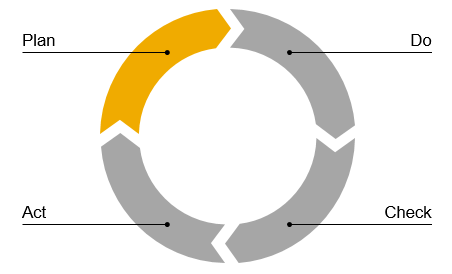
\includegraphics[width=9cm]{Abbildungen/pdca}
                    \caption{Deming-Zyklus}
                    \label{abb:pdca}
                \end{center}
            \end{figure}

            Der Zyklus wird in \autoref{abb:pdca} dargestellt. Der Startpunkt ist in Gold hervorgehoben und der Zyklus beginnt mit der Planung, wie der Prozess bzw. das Endprodukt, die Software, aussehen soll um danach die geplanten Prozesse zu durchlaufen. Am Ende dieser Durchläufe folgt die Prüfungsphase in der mit statistischen Methoden kontrolliert wird, ob die in der Planungsphase gesteckten Anforderungen erfüllt wurden. Auf Grundlage dieser Ergebnisse werden Maßnahmen beschlossen, um die Prozesse und Produkte zu optimieren und somit einen kontinuierlichen Verbesserungsprozess im Unternehmen zu etablieren.

            \subsubsection{Total Quality Management}

            \begin{quote}
              \enquote{TQM [Total Quality Management; Anm. d. Autors] is [seen] as a continuois process of improvement for individuals, groups of people and whole organisations.}\footnote{Kanji (Make ISO 9000 more effective), S.67.}
            \end{quote}

            Total Quality Management ist ein umfassendes Managementkonzept, dass die Grundlage für viele heute existierende Qualitätsmanagementsmodelle bildet. Es betrachtet neben den Anforderungen der Kunden und Mitarbeiter an die Qualität der Software, die Belange aller Stakeholder und die der Gesellschaft. Außerdem prüft es nicht nur die Eignung der Prozesse, um zum Ergebnis zu kommen, sondern auch die tatsächlich resultierten Ergebnisse.\footnote{Vgl. Krems (Total Quality Management).}

            Das Ziel ist ein Prozess der kontinuierlichen Verbesserung, der in der Literatur häufig als kontinuierlicher Verbesserungsprozess oder KVP bezeichnet wird. In japanischen Fabriken findet sich auch häufig das \emph{Kaizen} (Kai - Verbesserung, Zen - Zum Guten) als Qualitätsziel.

            Total Quality Management wird in Europa im Rahmen des European Quality Awards bewertet. Dieser bewertet das gesamte Unternehmen im Hinblick auf Qualitätskonzepte und gibt auf dieser Grundlage eine Bewertung zwischen 0\%und 100\% ab.\footnote{Vgl. Pfitzinger (ISO 9000 zu TQM), S.29ff.}

            \begin{figure}[!htbp]
                \begin{center}
                    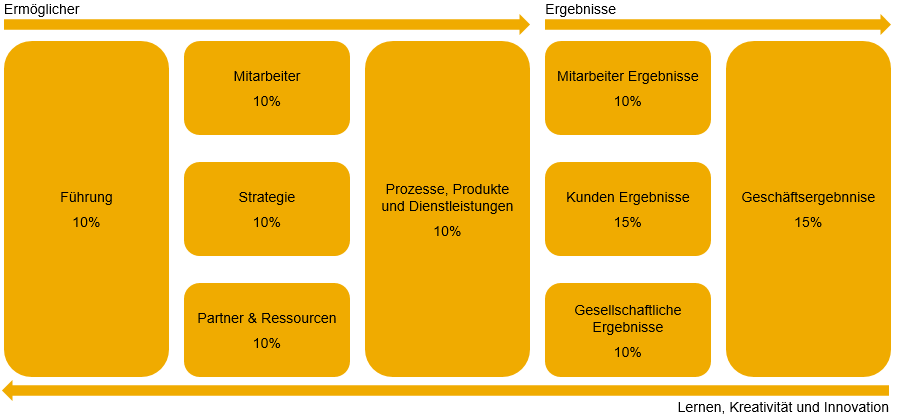
\includegraphics[width=\textwidth]{Abbildungen/efqmkat}
                    \caption[Kategorien zur Qualitätsbewertung von Unternehmen]{Kategorien zur Qualitätsbewertung von Unternehmen\protect\footnotemark}
                    \label{abb:efqm}
                \end{center}
            \end{figure}

            \footnotetext{Eigene Abbildung in Anlehnung an Pfitzinger (ISO 9000 zu TQM), S.30.}

            In \autoref{abb:efqm} werden die Kategorien der Bewertung von Qualität dargestellt. Die Ermöglicher auf der linken Seite nehmen dabei 50\% der möglichen Punkte ein, genau wie die Ergebnisse auf der rechten Seite. Die Ermöglicher bilden das Fundament der Qualität im Unternehmen und sind untereinander vernetzt. Hierbei geht eine umfassende Qualitätsstrategie von der Führung aus und muss von dieser gelebt werden. Von dort aus wird Spaltenweise gearbeitet. So werden die Mitarbeiter unter anderem von der Führung motiviert. Auch wird die Strategie zur Qualität von der Führung festgelegt.

            Nachdem der gesamte Prozess zwischen Ermöglichern und Ergebnissen durchlaufen und geprüft ist, kann die Führung auf Grundlage der Ergebnisse der Organisation nachjustieren und eine weitere Verbesserung anschließen. Somit beginnt ein Kreislauf, beziehungsweise eine kontinuierliche Verbesserung der Qualität.

            \subsubsection{Six Sigma}
            \label{subsec:sixsigma}

            Das Ziel Six Sigmas ist es \enquote{die Anforderungen des Kunden vollständig und profitabel [zu] erfüllen}\footnote{Knöfel (Six Sigma), S. 7}. Dabei ist neben dem externen Kunden, dem Abnehmer des Endprodukts, auch jeder interne Abnehmer eines Produktes gemeint. Sollte Abteilung B eines Unternehmens eine Fertigung von Abteilung A des gleichen Unternehmens weiterverarbeiten, so ist Abteilung B im Six Sigma Modell Kunde der Abteilung A. Auf diese Weise soll entlang der gesamten Prozesskette die Fehlerzahl gegen Null laufen.

            Six Sigma ist eine Methode, um möglichst perfekte Prozesse zu etablieren. Der Name dieser Methode entstammt der Statistik und entspricht der Zahl der Annahmequote von $6\sigma = 99.99966\%$. Dies bedeutet, dass beim Durchlauf von einer Millionen Prozessen, bzw. bei einer Millionen Endprodukte lediglich 3,4 Produkte fehlerhaft sind. Die Fehlerquote ist praktisch Null.\footnote{Vgl. Knöfel (Six Sigma), S.20f.}

            Um die Abweichungen zum Zielwert möglichst gering zu halten wird der Deming-Kreis, der im ISO 9001 Kapitel vorgestellt wurde, erweitert. Six Sigma verwendet den sogenannten DMAIC Verbesserungsprozess - Define, Measure, Analyse, Improve, Control - der aus dem Kaizen Prinzip entwickelt wurde. Der DMAIC Prozess wird durchlaufen, bis die Anforderungen des Kunden erfüllt wurden.\footnote{Vgl. Knöfel (Six Sigma), S.37ff.}

            \begin{figure}[!htbp]
                \begin{center}
                    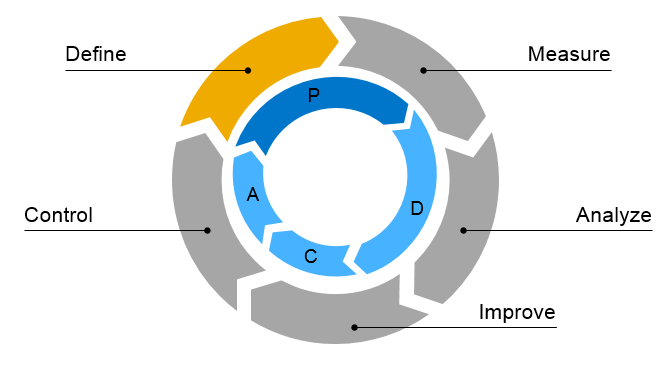
\includegraphics[width=11cm]{Abbildungen/pdcavsdmaic}
                    \caption{Kategorien zur Qualitätsbewertung von Unternehmen}
                    \label{abb:pdcavsdmaic}
                \end{center}
            \end{figure}

            In \autoref{abb:pdcavsdmaic} wird das Verhältnis des DMAIC Prozesses zum Deming-Kreis verbildlicht. In blau wird der Deming-Kreis mit den Phasen Plan, Do, Check und Act dargestellt, deren Anfangsbuchstaben in der Abbildung die jeweilige Phase markieren. Die Startpunkte der jeweiligen Zyklen sind jeweils farblich hervorgehoben.
            
            Im Folgenden werden die Phasen des DMAIC Prozesses vorgestellt und das jeweilige Äquivalent des Deming-Kreies erläutert.

            Zunächst wird die Problemstellung definiert. Das bedeutet, dass der Kunde befragt werden muss, welche Anforderungen er an den Prozess hat und welche Ausschuss- bzw. Fehlerrate er akzeptieren würde. Dies ist die Zielsetzung für den nachfolgenden Zyklus. Hierbei müssen die Kriterien messbar und binär, das heißt erfüllt oder nicht erfüllt, sein, damit in späteren Phasen geprüft werden kann, ob diese erfüllt sind.\footnote{Vgl. Knöfel (Six Sigma), S.42.} Die Definitionsphase des Prozesses stellt einen Teil der Planungsphase dar. Neben den Zielen wird auch die Vorgehensweise der nächsten Iteration geplant.

            Daraufhin wird das Maß festgelegt, an dem das Endergebnis gemessen wird. Die zuvor aufgenommenen Kundenanforderungen werden in statistische Messgrößen übersetzt und die zu messenden Kennzahlen festgelegt.
            Während eines Prozessdurchlaufs werden daraufhin Messdaten erfasst und gespeichert.\footnote{Vgl. Knöfel (Six Sigma), S.70.} Die Planungsphase erstreckt sich bis in die Messung hinein, da zu Beginn dieser Phase Verfahren zur Messung festgelegt werden. Die tatsächliche Messung findet im Rahmen der durchführenden (\emph{Do}) Phase statt und halten die Ergebnisse des durchlaufenen Prozesses fest.

            Die erfassten Daten werden nun analysiert und die Ursache der Abweichungen vom Zielwert wird erfasst.\footnote{Vgl. Knöfel (Six Sigma), S.124.} Die Analyse wird im Rahmen der \emph{Do} Phase durchgeführt und die Ergebnisse werden festgehalten, um der \emph{Improve} Phase als Grundlage zu dienen.

            Auf Grundlage dieser Abweichungen werden Verbesserungsvorschläge erarbeitet und der Mehrwert eben dieser wird beziffert. Zu beachten ist, dass die Ursache bekämpft werden soll und nicht die Symptome.\footnote{Vgl. Knöfel (Six Sigma), S.37.} Der bisherige Prozess wird geprüft (\emph{Check}), indem die Ergebnisse der Analyse mit den Wünschen der Planung und den vergangenen Iterationsergebnissen verglichen werden. Neben der Kontrolle, ob eine Verbesserung gegenüber früheren Iterationen vorliegt, können Möglichkeiten herausgearbeitet werden, um den Ablauf zu verbessern.

            Zuletzt werden Steuerungs- und Kontrollmöglichkeiten eingeführt, damit der verbesserte Prozess nachhaltig und konsistent umgesetzt wird. Das Six Sigma Team zieht sich zurück und überlässt die Kontrolle und den Prozess der ausführenden Abteilung.\footnote{Vgl. Knöfel (Six Sigma), S. 37.} Die Einführung dieser Verbesserungsmöglichkeiten und die Durchführung von Kontrollen deckt sich mit der \emph{Act} Phase des Deming-Kreises. 
    \chapter{Entwicklung eines Qualitätssicherungsprozesses für agile Prozesse}
\label{cha:prozessentwicklung}

    Im Folgenden werden die Vor- und Nachteile der agilen Entwicklungsverfahren erarbeitet und miteinander verglichen. Daraus wird abgeleitet welche Kriterien für Softwarequalität mit agilen Prozessen verfolgt werden und für welche Charakteristiken ein Qualitätssicherungsansatz verfolgt werden muss. Daraufhin werden Möglichkeiten gezeigt, wie dieser Qualitätssicherungsansatz in die agile Methode einfließen kann.

    \section{Grenzen der agilen Entwicklung}

        Agile Vorgehensweisen lösen einige Probleme, sind aber keine universelle Lösung für Herausforderungen in Softwareprojekten. Vor jedem Projekt muss sich das verantwortliche Team Gedanken machen, ob eine agile Vorgehensweise angebracht und zielführend ist, oder ob zu konventionellen Methoden gegriffen werden sollte. Im Rahmen dieses Abschnitts soll eine Checkliste entwickelt werden, die dem verantwortlichem Team die Entscheidung erleichtern soll. Hierzu werden die Vor- und Nachteile der agilen Methoden gegenüber der traditionellen Softwareentwicklung im prozeduralen Ansatz betrachtet.

        Agile Entwicklungsmethoden sind mit dem Ziel entstanden schnell und kostengünstig auf geänderte Anforderungen zu reagieren, da die traditionelle Softwareentwicklung an einem strukturierten Planungsprozess mit anschließender Entwicklung und abschließendem Test festhält. Als erste These lässt sich daher ableiten, dass eine agile Methode angebracht ist, wenn die Anforderungen zu Beginn des Projektes nicht feststehen oder absehbar ist, dass sich diese während der Projektlaufzeit häufig ändern werden.
        Sollten die Anforderungen zu Beginn des Projektes feststehen und kann davon ausgegangen werden, dass sich diese im Rahmen des Projektes nicht verändern, sollte eine traditionelle Herangehensweise bevorzugt werden.

        Ein weiterer Vorteil von agilen Entwicklungsmethoden ist, dass im Rahmen einer Iteration stets ein lauffähiges Inkrement erstellt wird, dass potenziell an den Kunden ausgeliefert werden könnte. Dies erleichtert die Entscheidung das Projekt zu einem bestimmten Zeitpunkt oder bei Überschreiten eines bestimmten Budgets zu stoppen, da zu jedem Zeitpunkt ein fertiges Produkt besteht, dass die Funktionen mit der höchsten Priorität besitzt. Sollte das Projekt daher eine fixe Deadline oder einen engen Budgetrahmen haben, kann durch agile Entwicklungsmethoden die Wahrung dieser Vorgaben erleichtert werden.
        Wenn das Projekt jedoch sicherheitskritisch ist, exakter Spezifikation bedarf und umfangreiche Anforderungen hat, die erfüllt werden müssen, dann sollte sich an das Projekt eine lange und umfassende Testphase anschließen, um das Softwareprodukt zu validieren. So ist zum Beispiel bei Regierungsbehörden häufig die Funktionalität und Sicherheit höher gewichtet als das Budget und die Laufzeit. In diesem Fall ist ein traditioneller Ansatz angemessener, da sich die vollständige Erfüllung der Spezifikation bei einem umfassend geplanten Softwareprodukt leichter messen und überpüfen lässt als in einer Menge von Inkrementen.\footnote{Vgl. Leffingwell (High Assurance and Regulated Environments), S.2ff.}

        Wie in den vorherigen Kapiteln vorgestellt, ist es empfehlenswert, dass die Entwicklungsteams lokal zusammen arbeiten, um die Kommunikation und den Austausch zu fördern. Große räumliche Distanzen mindern die Effektivität der Methoden. Außerdem ist die Teamgröße bei etwa 12 Personen gedeckelt. Es gibt Fälle, in denen mehrere Scrumteams in einem großen Scrumteam organisiert sind und somit mehr Entwickler ein Projekt bearbeiten, aber der Verwaltungsaufwand wird hierdurch erhöht und die Produktivität vermindert. Agile Entwicklungsmethoden sind somit nur empfehlenswert, wenn eine überschaubare Anzahl an Entwicklern an einem Ort zusammenarbeit.
        Für sehr große Teams und verteilte Entwicklung ist ein hierarchischer, planender Ansatz besser geeignet.

        Durch die hierarchische Struktur in klassichen Projekten, bei der ein fester Plan von einer kleinen Menge kompetenter Personen in untere Hierarchiebenen durchgereicht wird, wird nur eine kleine Menge an sehr geschulten und fachlich versierten Mitarbeitern benötigt. Zur Ausführung eines konkreten Plans ist kaum Kreativität nötig. Scrum Teams dagegen planen ihre nächsten Schritte selbst und entwickeln in jeder Iteration ihren eigenen Plan. Um jedes Fachgebiet adäquat abgedeckt zu haben, werden kreativ denkende Kollegen verschiedener Fachrichtungen in einem Team gebündelt und organisieren sich selbst. Dadurch, dass Scrum-Teams ihre Ideen selbst umsetzen werden insgesamt mehr kompetente Personen benötigt, sobald die Organisation auf agile Entwicklungsmethoden setzt.\footnote{Vgl. Dombrowski (Lean Development), S.75ff.}
        Sollte eine hohe Anzahl an kompetenten Angestellten vorhanden sein, ist ein agiles Verfahren erfolgsversprechender.

        Ein letzter erfolgskritischer Punkt eines agilen Entwicklungsprojektes ist die ständige Verfügbarkeit eines Kunden, der die Entscheidungsgewalt hat, Vorgaben für das finale Produkt zu treffen. Sollte dieser nicht zur Verfügung stehen oder jegliche Entscheidungen in seinem Unternehmen abstimmen müssen, ist ein agiles Projekt gefährdet, da es ohne Kundenanforderungen keine Arbeitsgrundlage hat oder in Iterationen aufgehalten wird.

        \begin{table}
        \begin{tabularx}{\textwidth}{|X|c|c|}
          \hline
           & $\mbox{ }$Ja$\mbox{ }$ & Nein \\
          \hline
          Ständig wechselnde Anforderungen & $\Box$ & $\Box$ \\
          Feste Zeit-/Budgetvorgabe & $\Box$ & $\Box$ \\
          Lokale, kleine Entwicklungsteams & $\Box$ & $\Box$ \\
          Hohe Anzahl kompetenter Angestellter & $\Box$ & $\Box$ \\
          Ansprechpartner des Kunden & $\Box$ & $\Box$ \\
          \hline
        \end{tabularx}
        \caption{Checkliste zur Angemessenheit agiler Methoden}
        \label{tbl:checklist}
        \end{table}

        \autoref{tbl:checklist} fasst die oben erarbeiteten Ergebnisse zusammen. Sollte die Mehrheit der Punkte in der Tabelle \emph{Ja} anzeigen ist eine agile Entwicklungsmethode empfehlenswert. Andersherum verhält es sich genau gleich.

    \section{Vergleich der agilen Entwicklungsverfahren}

        Lean Software Development bildet für die Entwicklung einen Rahmen aus Prinzipien, die für jedes Projekt in Methoden und Anforderungen übersetzt werden müssen. Dies bietet zu Beginn eines Projektes die Freiheit das Rahmenwerk an die speziellen Anforderungen anzupassen. Wenn besonders umfangreiche Sicherheitsrichtlinien gesetzt werden, sind andere Methoden notwendig als bei einer möglichst schnellen Fertigstellung eines Produkts. Lean Software Development gibt dem Team die Möglichkeit ihren Methodensatz dahingehend anzupassen.

        Scrum setzt dagegen eine Managementmethodik fest, die die Kommunikation des Teams fördern und das Anforderungsmanagement optimieren soll. Durch eine Menge an vorher feststehenden Meetings und eines priorisierten Backlogs steht zu jedem Zeitpunkt fest, was im nächsten Sprint entwickelt wird. Die Sprints von vorher festgelegter Dauer minimieren den Stress der Entwickler, da sie sich nicht ständig an neue Anforderungen und Methoden gewöhnen müssen. Gleichzeitig bieten sie aber genügend Flexibilität, um auf den Kunden reagieren zu können.

        Extreme Programming verfolgt, wie der Name impliziert, einen sehr extremen Ansatz. Tests, Entwicklung und Flexibilität werden maximiert - teilweise zu Lasten der individuellen Freiheit. Durch einen sehr strikten Vorgehensansatz und festgelegte Methodiken, wird den Entwicklern Freiheit genommen mit dem Ziel die Ergebnisse zu optimieren. Extreme Programming trifft die Annahme, dass zu Beginn des Projektes nicht feststeht, wie das zu entwickelnde Produkt aussieht und daher die Anforderungen erst während der Projektlaufzeit festgehalten werden.

        Im Rahmen dieses Abschnitts werden die drei Vorgehensweisen verglichen. Die folgende Tabelle zeigt dabei die Ziele, Ansätze und Entwicklungsmethoden an:

        \begin{table}[H]
        \begin{tabularx}{\textwidth}{|p{2.5cm}|X|X|X|}
          \hline
            & Lean & Scrum & Extreme Programming \\
          \hline
          Ziele & Entscheidungen mit bestmöglichem Wissen treffen & Funktionen mit höchster Priorität erfüllen & Maximale Produktivität und Flexibilität
          \vspace{0.5\baselineskip} \\
          Ansatz & Ausprobierend, tastend & Dynamisch, Personenorientiert & Prozedural, Prozessorientiert
          \vspace{0.5\baselineskip} \\
          Entwicklungs-methode & Freie Methodenwahl & Freie Methodenwahl & Restriktiv, vorgeschrieben \\
          \hline
        \end{tabularx}
        \caption{Vergleich agiler Entwicklungsverfahren}
        \label{tbl:vergleich}
        \end{table}

        Wie in  \autoref{tbl:vergleich} zu sehen ist, hält das Extreme Programming mehr Restriktionen für die Entwickler bereit, während Scrum die Entscheidungsgewalt hinsichtlich der Methoden und Vorgehensweisen an das Scrum-Team weitergibt. Dadurch erhält ein Scrum-Team mehr Möglichkeiten aus den vergangenen Sprints zu lernen und Zeitpläne, Methodiken und Ziele im nächsten Sprint anders zu setzen. Wenn ein Extreme Programming Team dagegen feststellt, dass eine bestimmte User Story nicht umsetzbar ist, hat es keine Möglichkeit Einfluss auf die Methodik zu nehmen. Die Lean Software Development Vorgehensweise macht dagegen weder Vorgaben zur Entwicklung noch zum Management der Anforderungen und ist mit vorgegebenen Prinzipien die Allgemeinste der Methoden.

        Die Lean Methode kann durch Einsatz der Hilfsmittel aus Scrum und Extreme Programming ergänzt werden und nähert sich damit immer weiter den jeweiligen Methoden an. Aus den vorgegebenen Prinzipien zur Orientierung der Entwicklung wird dann eine Managementmethodik abgeleitet, die widerum zu einem ganzheitlichen Ansatz erweitert werden kann.

        Die agilen Vorgehensweisen lassen sich miteinander kombinieren, wobei eine sehr abstrakte Methode sich einer sehr konkreten Methode annähert, je mehr Werkzeuge sie dieser entnimmt.

        Da alle agile Methoden auf dem agilen Manifest beruhen, haben sie in ihren Kernannahmen viele Gemeinsamkeiten. Alle Methoden nehmen an, dass die Anforderungen an das Produkt zu Beginn der Entwicklung nicht feststehen und wollen somit möglichst flexibel auf Änderungen reagieren. Beim Lean Software Development wird es durch mehrere konkurrierende Entwürfe realisiert, die auf Grundlage einer, im laufenden Projekt erweiterten Faktenbasis. gefiltert werden, bis eine Entscheidung getroffen werden kann. Scrum und Extreme Programming setzen dagegen auf Iterationen, die die am höchsten priorisierten Wünsche des Kunden umsetzen und sich so dem Soll-Ergebnis annähern.

        Gemeinsam ist den Methoden außerdem, dass sie die Entwickler in den Mittelpunkt rücken. Alle agilen Methoden geben den Entwicklern einen Vertrauensvorschuss und erwarten Kreativität und Fachkenntnisse bei der Lösung. Im Gegensatz zu herkömmlichen Methoden wird der Plan und die Umsetzung von den ausführenden Personen beschlossen und nicht von einer kleinen Menge ranghöherer Angestellter.

        Unterschiede zwischen den Methoden sind darin begründet, dass sie an verschiedenen Ebenen ansetzen. Lean lässt sich auch auf Wasserfallmodelle anwenden und nicht nur auf iterative Methoden, da es nur Prinzipien vorgibt, an denen sich orientiert werden soll. Scrum gilt als Managementprozess, der die Entwicklung offen lässt. Extreme Programming ist allumfassend aufgesetzt.

        \begin{figure}[!htbp]
            \begin{center}
                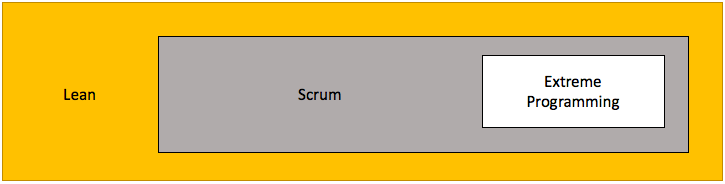
\includegraphics[width=11cm]{Abbildungen/ag_methoden}
                \caption[Umfang agiler Methoden im Vergleich]{Umfang agiler Methoden im Vergleich}
                \label{abb:vergleich}
            \end{center}
        \end{figure}

        \autoref{abb:vergleich} illustriert nochmals das Verhältnis der Verfahren. Je mehr Werkzeuge einer inneren Methode gewählt werden, desto mehr nähert sich das Verfahren dem Extreme Programming an. Da in dieser Arbeit agile, iterative Methoden betrachtet werden sollen, werden die Qualitätssicherungsmethoden auf die Scrum Vorgehensweise angewandt, da diese die am weitesten gefasste Methode ist, die Iterationen vorsieht. Die Methoden des Extreme Programmings und Prinzipien des Lean Software Developments werden, wenn nötig und angemessen, ergänzend hinzugezogen.

        Zu beachten ist, dass sich die in dieser Arbeit betrachteten Methoden nicht widersprechen. Die Prinzipien des einen Modells werden beispielsweise durch Methoden des Anderen umgesetzt. Im Folgenden wird die Scrum Methodik als Basis des Prozesses genutzt, falls es jedoch der Qualität zu Gute kommt, um Methoden des Extreme Programming oder Lean Software Developments ergänzt. Außerdem ist Scrum der in der SAP SE verwendete Ansatz agiler Entwicklungsmethoden.

    \section{Qualität durch agile Methoden}

        Dieses Kapitel zeigt, welche Qualitätsstandards für Software durch die Anwendung der agilen Methoden bereits erfüllt werden. Im Anschluss wird geprüft, wie die agilen Methoden durch Qualitätssicherungsmodelle ergänzt werden können, um eine umfangreiche und zufriedenstellende Softwarequalität zu gewährleisten.

        Wie im Grundlagenteil bereits erläutert wird sollte besonders viel wert darauf gelegt werden, dass eine Software funktional, verlässlich und wartbar ist.

        \subsection{Funktionalität}

            Funktionalität wird daran gemessen, dass Software die geforderten Funktionen sicher, genau und in Zusammenarbeit mit anderen Systemen erfüllt. Scrum liefert mit jedem Sprint eine potenziell auslieferbare Software, die vom Kunden bewertet wird, um die Richtung des Projektes zu steuern. Die am höchsten priorisierte, noch nicht realisierte Funktion wird dabei stets als das Ziel des nächsten Sprints definiert. Somit wird in den ersten Sprints eine Basisfunktionalität geliefert, die ständig erweitert wird. Das Projekt kann beendet werden, sobald alle Anforderungen an die Funktionalität erfüllt sind. Agile Methoden liefern somit ein wichtiges Fundament zur Erstellung von funktionaler Software. Im Gegensatz zu klassischen Methoden der Softwareentwicklung kann der Kunde die Software am Ende des Projektes in jedem Fall einsetzen und müsste bei vorzeitigem Projektende lediglich mit einem reduzierten Funktionsumfang auskommen. Die Passgenauigkeit (\emph{Suitability}) ist also sehr hoch.

            Um die Akkuranz (\emph{Accuracy}) der Software zu gewährleisten muss sie stets die erwarteten Resultate und Effekte erzielen, die sich der Anwender von der Funktion erhofft. In der Scrum-Entwicklung werden die erwarteten Effekte vom Product Owner dargestellt und vom Team ausgearbeitet. Hier erscheint es vorteilhaft die User-Stories und Unit-Tests des Extreme Programming zu verwenden. Der Anwender beschreibt seine Aufgabe, seine Eingaben in die Software und die erwartete Ausgabe. Diese werden in Unit-Tests umgesetzt und ein erfüllter Unit-Test entspricht bei konsequenter Umsetzung einer Rückgabe der erwarteten Resultate. Auch die Akkuranz lässt sich durch den Einsatz agiler Methoden sicherstellen.

            Die Zusammenarbeit mit anderen Systemen (\emph{Interoperability}) ist abhängig von der umliegenden Architektur. Im Falle von einer serviceorientierten Architektur können sehr gut Datenflüsse zwischen den Systemen simuliert werden, um so User-Stories und Unit-Tests zu erfüllen. Bei einer direkten Anbindung an historisch gewachsene Altsysteme, die beispielsweise zum Reporting für Kennzahlen dienen, erweist sich der Test schwerer, da diese in der Entwicklungsumgebung meist nicht zur Verfügung stehen. Die Kommunikation an Schnittstellen muss daher vor Beginn der Entwicklung eines Moduls spezifiziert werden. Ein umfangreicher Test eben dieser kann erst bei der Integration in die Landschaft des Kunden erfolgen. Hier sollten weitere Qualitätssichernde Maßnahmen gestartet werden.

            Zuletzt ist im Rahmen der Funktionalität die Sicherheit (\emph{Security}) zu beachten. Es ist sicherzustellen, dass unauthorisierte Personen und Systeme keinen Zugriff und authorisierte Nutzer und Systeme Zugriff auf die betreffenden Systeme haben. Wie in ISO 9126-1 als Notiz angemerkt ist Sicherheit \enquote{a characteristic of quality in use, as it does not relate to software alone, but to a whole system.}\footnote{ISO 9126-1 (Information Technology), S.8} Die Software kann nicht am Ende eines Sprints auf Sicherheit geprüft werden. Um die Sicherheit zu garantieren, muss das vollständig auslieferbare Produkt zuzüglich aller Schnittstellen zu Umsystemen geprüft werden. Dies kann ebenfalls nicht im Rahmen eines agilen Prozesses ablaufen.

            Für die Funktionalität bedeutet dies, dass agile Prozesse die gewünschten Funktionen und Ausgaben produzieren, aber die Zusammenarbeit mit umliegenden Systemen und die Sicherheit des gesamten Systems separat geprüft und sichergestellt werden sollte.

        \subsection{Verlässlichkeit}

            Bei Unternehmen der Finanzdienstleistungsbranche ist es unerlässlich, dass Software stets wie erwartet reagiert und ungültige Eingaben herausfiltert, da Fehler in der Software die Kundenzufriedenheit, und somit auch das Kundenvertrauen, senken können und bei Berechnungen von beispielsweise Kontoständen auch Rundungsfehler sehr große Abweichungen nach sich ziehen. Unit-Tests vergleichen die Resultate der Software mit erwarteten Ergebnissen und geben auf Grund dieses Vergleiches einen erfolgreichen Test zurück oder einen Fehler. Somit wird zumindest auf erwartete Ergebnisse geprüft.

             Abgesehen von der Richtigkeit produzierter Ergebnisse, muss auch überprüft werden, ob das Produkt allgemein keine Fehler auf Grundlage von Fehlern im Programm wirft. Die Reife (\emph{Maturity}) eines Softwareproduktes wird daran gemessen, dass der Programmablauf in sich fehlerfrei ist. Ein Scrum-Team testet sehr viel und durchläuft die Software durch automatisierte Tests sehr häufig, bevor es diese zum Kunden ausliefert. Durch viele automatisierte Tests sollten alle Fehler der Software noch während der Entwicklung zum Vorschein kommen und eliminiert werden können. Fehler in der Software werden somit schon während der Entwicklung abgefangen.

            Die Fehlertoleranz (\emph{Fault tolerance}) einer Software gibt an, wie sehr sie von ungültigen Eingaben, falscher Kommunikation von Seiten der Schnittstellen und Hardwarefehlern abhängig ist. Das Ziel der Software sollte es sein Fehler zu entdecken und zu melden, um die Vermeidung, beziehungsweise Korrektur, eben dieser zu erleichtern. Ein Ausfall der Hardware kann von Seiten der Entwickler nicht verhindert werden. Die Sicherheitsmaßnahmen gegen Hardwaredefekte werden im nächsten Absatz behandelt. Empfohlen werden lediglich redundante Hardwarekomponenten, sodass kein Single-Point-of-Failure existiert. Falsche Kommunikation der Schnittstellen kann ebenfalls nicht durch das Scrum-Team verhindert werden, da dieses die Schnittstellen nicht vor Ort testen kann um mögliche Fehler auszuprobieren. Die Prüfung von Schnittstellen und Hardware sollte somit im Rahmen eines umfassenden Integrationstest stattfinden.
            Falsche Benutzereingaben lassen sich bereits während des Tests abfangen, indem eine Prüfung die Eingaben validiert und mit erwarteten Eingaben vergleicht. Hier werden neben den automatisierten Tests umfassende Gültigkeitstests benötigt.
            Die Reaktion der Software auf fehlerhafte Eingaben sollte am Ende der Entwicklung umfangreich getestet werden.

            Zuletzt sollte bei einem Defekt ein sicherer und korrekter Zustand des Systems möglichst schnell wiederhergestellt (\emph{Recoverability}) werden. Dies setzt regelmäßige Back-Ups und eine redundante Datenhaltung voraus. Während der Entwicklung sollte daher geprüft werden, wie sich die Software verhält, wenn sie unerwartet unterbrochen wird, beispielsweise durch einen Stromausfall. Die häufigsten und bekanntesten Ausfallszenarien von Software, wie Netzwerkfehler, menschliche Fehler, Stromaufall und Wetterunfälle\footnote{Vgl. Statista (Ursachen von IT-Ausfällen).} lassen sich sehr gut replizieren, testen und daher abfangen. Sie sollten daher in produktiver Software nicht vorgefunden werden.

            Die Verlässlichkeit der Software im Hinblick auf ungültige Eingaben sollte vor Produktivsetzung geprüft werden. Die Wiederherstellbarkeit und Reife der Software lassen sich jedoch in der Entwicklungsumgebung sicherstellen.

        \subsection{Wartbarkeit}

            Extreme Programming empfiehlt bei der Entwicklung der Software keine zukünftigen Erweiterungen im Code zu ermöglichen. Dies geschieht unter der Annahme, dass eine einfach gehaltene Software ohne überflüssigen Code leichter zu erweitern ist, als eine umfangreiche Software, die speziell auf Erweiterungen ausgelegt ist, die vielleicht nie genutzt werden. Der inkrementelle Ansatz von Scrum und Extreme Programming bedeutet, dass eine Vielzahl an Bausteinen entsteht, die miteinander und in das bestehende System integriert werden. Wenn ein neues System an einen bestimmten Baustein angeschlossen werden muss, kann es sein, dass daher nur ein Glied dieser modularen Systemkette verändert werden muss, statt ein umfassendes System.

            Als erster Teil der Wartung wird vorgesehen, dass das bestehende System analyisiert (\emph{Analyzability}) werden kann. Dies bedeutet, dass der Code auf Fehler untersucht wird, oder geprüft wird, ob Veränderungen notwendig sind. Ein Vorteil der agilen Vorgehensweisen ist, dass die Dokumenation direkt im Code stattfindet und somit keine veralteten Dokumente als Grundlage dieser Analyse dienen. Im Extreme Programming gehört der Code zudem allen Entwicklern. Somit ist es möglich, dass mindestens ein Entwickler verfügbar ist, der Fragen beantworten kann. Die Verständlichkeit und analysierbarkeit des Codes ist bei konsequenter Umsetzung der agilen Prinzipien sehr hoch.

            Während der agilen Entwicklung und insbesondere beim Extreme Programming wird der Code ständig neu strukturiert beziehungsweise Refactored. Die Gliederung des Hauptprogramms in eine Menge von Methodenaufrufe erleichtert es, Teile der Software zu verändern (\emph{Changeability}). Die Modularisierung der Software in wiederverwendbare Methoden erleichtert zudem die Korrektur von Fehlern, da diese nur an einer Stelle stattfinden muss. Der Code ist darauf ausgelegt ständigen Veränderungen unterworfen zu sein. Hiermit ist auch die Veränderbarkeit in einem agil entwickelten Softwareprodukt gegeben.

            Im Rahmen von Unit-Tests kann überpüft werden, ob sich das Verhalten der Software auf Grund von Änderungen im Code geändert hat. Sollten diese Unit-Tests nach einer Veränderung keine korrekten Ergebnisse liefern muss der Code weiter angepasst und der Fehler gesucht werden. Die Stabilität (\emph{Stability}) der Software, dass heißt, die Fähigkeit unerwartete Effekte von Veränderungen zu verhindern, ist sehr hoch.

            Zuletzt ist gefordert, dass veränderte Software validiert werden kann (\emph{Testability}). Eine Softwarevalidation ist der \enquote{Prozess des Bestätigens, dass die Spezifikation einer Phase oder des Gesamtsystems passend zu oder konsistent mit den Anforderungen des Kunden ist.}\footnote{Bresser (Validierung und Verifikation).} Die Software wurde zusammen mit einem Kunden auf Grundlage von direkter Kommunikation und, falls angewandt, User-Stories und Unit-Tests entwickelt. Ein Vergleich mit einer Spezifikation ist nicht möglich, da diese nicht angelegt ist. Um, wie von den agilen Prinzipien vorgeschrieben, keine allzu umfassende Dokumentation der Anforderungen anfertigen zu müssen, ist es empfehlenswert die Validierung der Anforderungen anhand von existierenden Dokumenten zu erledigen. Die Anforderungen des Kunden werden vom Product Owner im Backlog zusammengefasst und auf Grundlage dieses Backlogs werden die Funktionen, die die Software besitzen soll, priorisiert und in das Entwicklungsteam hereingetragen. Der Backlog stellt somit alle Anforderungen dar, die der Kunde gestellt hat. Am Ende jedes Sprints wird das fertige Inkrement dem Kunden vorgestellt und dieser gibt sein Feedback dazu ab. Wie zuvor beschrieben muss bei der Anfertigung des Backlogs ein klares Bild beim Entwicklungsteam und beim Kunden bestehen, was als Definition von \emph{Done} festgelegt ist. Gibt der Kunde daher nach einem Sprint sein \emph{Done} zu einem Produkt, kann es im Backlog als erledigt markiert werden. Um am Ende die Anforderungserfüllung zu überprüfen, muss nur der Backlog vorgelegt werden.

            Zusammenfassend lässt sich sagen, dass die Wartbarkeit des Codes und des Softwareproduktes allgemein durch agile Methoden deutlich erleichtert wird. Der modulare Aufbau des Systems ermöglicht zudem die Integration und Einbindung von neuen Systemen.

    \section{Qualitätssichernde Erweiterung der agilen Methoden}

        %Zunächst werden die Punkte notiert, wo zusätzliche QUalitätssicherung von Nöten ist. An dieser Stelle wird erklärt wie es bei der herkömmlichen Softwareentwicklung gelöst wird und welche Methoden der Qualitätssicherung, bpsw. des Testens angewandt werden können. Wenn alle groben Probleme abgedeckt sind kann man sich an Null-Fehler / Dokumentation wie in ISO 9000 gefordert verrennen.

        Wie im letzten Abschnitt erarbeitet sollten folgende Punkte durch zusätzliche Qualitätssicherungsmethoden ergänzt werden, um auch in agilen Projekten Qualität sicherzustellen.

        \begin{itemize}
          \item Functionality
            \begin{itemize}
              \item Interoperability
              \item Security
            \end{itemize}
          \item Reliability
            \begin{itemize}
              \item Fault Tolerance
            \end{itemize}
          \item Maintainability
        \end{itemize}

        In \autoref{subsec:kritchar} werden die kritischen Sub-Charakteristiken beleuchtet und beispielhaft Vorgehensweisen der Qualitätssicherung und der klassischen Softwareentwicklung vorgestellt, die den unsicheren Ergebnissen der agilen Entwicklung entgegen wirken.

        \subsection{Kritische Charakteristiken}
        \label{subsec:kritchar}

            \subsubsection{Interoperabilität}

                Um die Interoperabilität der Software mit den umliegenden Systemen zu gewährleisten, müssen die Schnittstellen spezifiert werden. Eine Herausforderung, die bei der agilen Entwicklung besteht ist, dass die Software in enger Zusammenarbeit mit genau einem Kunden entwickelt wird, um diese genau auf seine Wünsche zuzuschneiden. Da die SAP SE ein Anbieter von Standardsoftware und kein Anbieter von Individualsoftware ist, muss die Software nach Fertigstellung bei einem Referenzkunden generalisierbar sein, um relevant zu bleiben.

                \begin{table}[H]
                    \begin{tabularx}{\textwidth}{|X|X|}
                        \hline
                        Herausforderung & Lösungsansatz \\
                        \hline
                        Kommunikation mit umliegenden Systemen & Schnittstellenlandkarte zu Beginn des Projekts erarbeiten \\
                        \vspace{0.5\baselineskip}
                        Wiederverwendbare Schnittstellen & \vspace{0.5\baselineskip} Verwendung anerkannter Standards zur Interoperabilität (Web-Services) \\
                        & Dokumentation der entwickelten Schnittstellen \\
                        \hline
                    \end{tabularx}
                    \caption{Lösungsansatz zur Interoperabilität}
                \end{table}

                Bei einem klassischen Softwareprojekt im Rahmen der Accelerated SAP Methodik wird zu Beginn des Projektes eine Service- und Schnittstellenlandkarte erstellt, die alle bestehenden Systemen auflistet und zeigt, welche Schnittstellen in der neuen Software benötigt werden.
                Dies ist eine manuelle Aufgabe, die von Experten des Systems in Zusammenarbeit mit SAP Experten ausgearbeitet wird. Es werden alle Systeme aufgelistet und auf Grundlage dieser die Schnittstellen von und zu diesen dokumentiert. Dabei wird notiert wer eine Schnittstelle wann benutzt. Mit diesem System- und Schnittstellendokument kann das Scrum-Team die Software aufbauen und mit Testdaten befüllen. Im Idealfall wird eine technologieunabhängige Kommunikation etabliert, beispielsweise über Web-Services.

                \begin{quote}
                    \enquote{Companies that regularly hand off data between systems such as those in the financial services, energy trading, high-tech manufacturing, and telecommunications industries are ideal candidates for Web services technologies.}\footnote{Chung (Web Services Computing), S.36.}
                \end{quote}

                Genau spezifizierte Schnittstellen auf Grundlage von Web-Services bieten den Vorteil, dass die Datentypen unabhängig von Anfragenden und Antwortenden sind, indem die Nachrichten über einen Enterprise Service Bus geroutet und von ihm übersetzt werden. Mit der Einführung einer Orchestrierungsebene bei jeder neuen Softwareeinführung ist die Implementierung des Scrum-Teams technologie-, system- und kundenunabhängig und eine, in diesem Fall auch außerhalb des Quellcodes gut dokumentierte Anforderung an Services, genügt für eine Integration.

                Das Ergebnis einer solchen, konsequent umgesetzten Vorgehensweise, ist eine modulare, serviceorientierte Architektur. Durch dies können einzelne Komponenten ersetzt werden, sobald das jeweilige Modul im Rahmen eines Sprints fertig gestellt ist. Die Funktionalität jeder Komponente kann daher in einer produktiven Umgebung getestet werden, indem ein neues Modul ohne tatsächliche Verantwortung, Daten bezieht und wieder zurück gibt. Diese können dann mit der bestehenden Software oder den erwarteten Ausgaben verglichen werden kann.

                Um Interoperabilität, wie im oben aufgeführten Beispiel, zu erreichen, sollte das Scrum-Team mit Hilfe eines Referenzkunden eine standardisierte, technologieunabhängige Kommunikation anstreben, die, außerhalb des Codes, verständlich dokumentiert wird. Eine Verwendung von anerkannten Standards wird ebenfalls im Rahmen der ISO 9126-1 empfohlen.\footnote{Vgl. ISO 9126-1 (Information Technology), S.9.}

            \subsubsection{Sicherheit}

                Die Sicherheit von Software kann auf zwei Wegen gewährleistet werden. Durch eine Verifikation und Validierung werden Fehler aufgedeckt, die im Rahmen der Entwicklung entstanden sind und durch nachträgliche Korrektur eliminiert werden können. Die zweite Vorgehensweise ist die Software Security Assurance, die Fehler während der Entwicklung vermeiden soll. Konform zum Six Sigma Prinzip, dass fehlerfreie Prozesse als Grundlage für fehlerfreie Resultate sieht, sollte die Ursache bekämpft werden statt nachzubessern. Der Fokus während der Entwicklung sollte daher auf die Software Security Assurance gelegt werden. Eine nachträgliche Prüfung ist dennoch empfohlen. Ein verantwortungsvoller Umgang der Anwender der Software wird vorausgesetzt, da das Scrum-Team keinen Einfluss auf die Mitarbeiter des Unternehmens nehmen kann.

                \begin{table}[H]
                    \begin{tabularx}{\textwidth}{|X|X|}
                        \hline
                        Herausforderung & Lösungsansatz \\
                        \hline
                        Sicherheitsfehler vermeiden & Aufnahme von Sicherheitsexperten im Entwicklerteam \\
                        & Sichere, verifizierte Standards verwenden \\
                        & Vorschriften der bestehenden Software beachten \\
                        & Doppelte Kontrolle durch Pair Programming \\
                        & Sicherheit als User-Story \\
                        \vspace{0.5\baselineskip} Sicherheit überprüfen & \vspace{0.5\baselineskip} Sicherheit dokumentieren \\
                        & Umfangreiche Systemtests nach Vollendung des Projekts \\
                        & Formale Validierung und Verifikation \\
                        \hline
                    \end{tabularx}
                    \caption{Lösungsansatz zur Sicherheit}
                \end{table}

                Sicherheit kann, und muss, auf der System- und der Softwareebene sichergestellt werden. Die Systemebene setzt hauptsächlich auf Verschlüsselung und Zugriffskontrollen, während die Softwarebene ausnutzbare Lücken im Quelltext vermeiden soll.

                Maßnahmen auf der Systemebene umfassen unter anderem Firewalls, Daten- und Netzwerkverschlüsselung, Zugriffskontrollen und Authorisierungs- bzw. Authentifizierungsmechanismen. Die Sicherheit auf Systemebene muss nach Fertigstellung der einzelnen Softwarekomponenten entwickelt werden und allumfassend sein.\footnote{Vgl. Goertzel (Enhancing the development life cycle), S.6.}
                Für die Iterationen sollte nur Wert auf eine sichere Kommunikation zwischen den Modulen des Systems gelegt werden. Diese sollte durch die oben genannten Kommunikationsstandards gewährleistet sein. Wenn Vorschriften und Sicherheitsmerkmale in dem System bestehen, in das die Software eingebettet werden soll, dann müssen diese an das Scrum-Team herangetragen werden und in der Entwicklung beachtet werden.

                Angreifbare Schwachstellen in der Software zu vermeiden ist die Aufgabe des Scrum-Teams. Zur Vermeidung von offensichtlichen Mängeln kann die Extreme Programming Technik des Pair Programmings angewandt werden. Durch zwei Entwickler, die den Quellcode kontrollieren, und ständig überprüfen, kann eine erste Menge von Mängeln abgefangen werden. Die Aufmerksamkeitsspanne von zwei Personen ist größer und somit werden Flüchtigkeitsfehler unterbunden.

                Um weitere Fehler zu vermeiden, und die Sicherheit der Software zu garantieren, wird eine umfangreiche Dokumentation vorausgesetzt. Die Dokumentation einer sich ständig verändernden Software ist ein umfangreiches und zeitintensives Projekt, sodass effizientere Methoden gefunden werden müssen. Eine Möglichkeit, um die Sicherheit der Software in den Rahmen eines agilen Projektes einzugliedern ist die Sicherheit als User-Story.\footnote{Vgl. Wäyrynen (Security Engineering), S.11.} Dies kann dabei eine klassische User-Story sein, wie zum Beispiel: \emph{Als Anwender möchte ich eine Software verwenden, die unzulässige Eingaben von mir abfängt und keinen unabsichtlichen oder absichtlichen Schaden durch meine Interaktion zulässt}. Eine andere Möglichkeit sind Misuse-Stories, die schädliches Verhalten eines Anwenders simulieren und abfangen müssen.

                Ergänzend kann die Aufnahme eines Sicherheitsexperten in das Entwicklerteam die allgemeine Aufmerksamkeit gegenüber der Sicherheit erhöhen und ist daher auch empfehlenswert.

            \subsubsection{Fehlertoleranz}

                Vor der Fehlertoleranz von Software steht die Fehlervermeidung. Jeder Fehler, der während der Entwicklung abgefangen wird, muss nicht während der Laufzeit des Programms behandelt werden. Hierfür bieten die agilen Verfahren, die auf Grundlage des Test-Driven Developments arbeiten, sehr gute Methoden durch automatisierte Tests, die sehr häufig laufen und die meisten Erwartungswerte abdecken. Automatisierte Tests sind meistens Black-Box Tests, die das Ergebnis eines Methodenaufrufs mit erwarteten Ergebnissen vergleichen. Im Rahmen eines Black-Box Tests müssen alle möglichen Eingaben eines Anwenders abgedeckt werden. So müssen auch ungültige Eingaben getätigt werden, um zu prüfen, ob diese erfolgreich abgefangen werden.
                Eine weitere Möglichkeit neben dem Black-Box Test bietet der in \autoref{subsec:analytischeqs} vorgestellte Strukturtest einer Software. Dieser ist durch Unit-Tests nicht abgedeckt und nur das Pairprogramming bietet eine Annäherung zum White-Box Test. Eine Durchführung von Strukturtests während der Entwicklung sollte in regelmäßigen Abständen stattfinden, beispielsweise am Ende jeder Woche.
                Eine Kombination dieser beiden Tests führt dazu, dass Mängel der Ergebnisberechnung und Mängel des Codes weitgehend eliminiert werden.

                \begin{table}[H]
                    \begin{tabularx}{\textwidth}{|X|X|}
                        \hline
                        Herausforderung & Lösungsansatz \\
                        \hline
                        Vermeidung von Softwarefehlern & Unit-Tests (Test-Driven Development) \\
                        & Regelmäßige Strukturtests \\
                        \vspace{0.5\baselineskip} Toleranz gegenüber Softwarefehlern & \vspace{0.5\baselineskip} Redundantes Auführen von Operationen \\
                        & Unabhängige, konkurrierende Algorithmen implementieren \\
                        \vspace{0.5\baselineskip} Missbrauch von Schnittstellen verhindern & \vspace{0.5\baselineskip} Kommunikation von und zur Softwarekomponente spezifieren \\
                        & Verwenden von Kommunikationsstandards \\
                        \hline
                    \end{tabularx}
                    \caption{Lösungsansatz zur Fehlertoleranz}
                \end{table}

                Die Möglichkeit, dass der Code Lücken enthält oder nicht alle Sonderfälle abgedeckt sind, besteht trotz der beiden Testverfahren. In diesen Fällen muss die Fehlertoleranz verhindern, dass der Anwender falsche, ungültige oder keine Ergebnisse erhält.

                Um die Sicherheit und Ausfallwahrscheinlichkeit von Hardware zu minimieren, werden alle Module redundant installiert, sodass der Ausfall eines Teils nicht das System zum Einsturz bringt. Genau wie bei Hardware kann es auch bei Software hilfreich sein redundante Operationen laufen zu lassen. Software ist im Gegensatz zu Hardware von zufälligen Ausfällen unabhängig und reagiert auf die gleiche Eingabe mit der gleichen Ausgabe.\footnote{Vgl. Chen (N-Version Programming), S.113.} Es kann dennoch vorteilhaft sein ein Programm zur gleichen Zeit mehrfach zu starten und die Ergebnisse zu vergleichen, da Servereingaben oder Informationen aus anderen Systemen unvollständig ankommen könnten oder, bei Thread-basierten Systemen, Schreib- und Leseprozesse blockiert werden könnten, was bei manchen Anwendungsfällen nicht auffällt. Damit die konkurrierenden Prozesse absolut unabhängig voneinander arbeiten, müssen sie individuell implementiert sein und auf eigenen Datenbasen arbeiten. Je mehr Prozesse gleichzeitig redundant ablaufen, desto höher ist die Wahrscheinlichkeit das korrekte Ergebnis zu erhalten.

                Ergänzend hierzu kann die selbe User-Story mit verschiedenen Algorithmen umgesetzt werden. Dies erfordert zwar den doppelten Code-Aufwand, da die beiden Lösungen absolut unabhängig sein sollen, erhöht aber weiterhin die Fehlertoleranz. Die Entwicklung von konkurrierenden, unabhängigen Algorithmen sollte daher nur bei höchst kritischen Projekten angewandt werden.
                Probleme aufgrund von Softwarefehlern werden durch oben genannte Methoden auch in agilen Projekten weitestgehend eliminiert.

                Um zu gewährleisten, dass das Programm durch vorsätzlichen Missbrauch von Schnittstellen nicht angegriffen wird, sollte die Kommunikation von und zur Software spezifiziert werden. Hier bieten sich die zuvor erwähnten Web-Services an, die eine standardisierte Anfrage an die Software zulassen und eine Antwort festlegen. So kann sich das angesprochene System und das anfragende System sicher sein, gültige und valide Daten zu erhalten. Software, die mit Anwendereingaben arbeitet, kann ähnlich vorgehen, da die Anfragen bei der häufig verwendeten 3-Schichten-Architektur ebenfalls von außen an das System herangetragen werden.

                Um die Fehlertoleranz einer Software sicherzustellen, sollten daher zunächst präventive Maßnahmen ergriffen werden, da ein Fehler nie vollständig umgangen werden kann. Konventionen und Standards helfen jedoch dabei möglichst wenig Fehler zu machen, da diese durch eine Vielzahl von Personen geprüft und getestet wurden und somit die höchste Zuverlässigkeit bieten - insbesondere bei der Kommunikation zwischen Modulen und Systemen. Für die Kommunikation zwischen Finanzanwendungen hat das Banking Industry Architecture Network zudem ein Rahmenwerk veröffentlicht, dass neben einheitlichen Kommunikationsstandards ein einheitliches Datenmodell vorgibt. Somit kann auch die Art der zu übertragenden Arten genau spezifiziert werden. 
    \chapter{Etablieren der Qualitätssicherung in agilen Prozessen}

    Das Ziel dieses Kapitels ist es eine Möglichkeit aufzuzeigen, die zuvor herausgearbeiteten Ansätze, in ein agiles Projekt zu integrieren und kontinuierlich zu verbessern. Hierfür werden Methoden und Ziele aus ISO 9000ff., Total Quality Management und Six Sigma kombiniert. Die Ansätze können in kleinen Schritten iterativ in den Scrum-Prozess integriert werden und der durch sie erzielte Fortschritt unmittelbar überprüft werden.

    Die Grundlage zur kontinuierlichen Verbesserung von Sprints im Scrum soll der im Rahmen von \autoref{subsec:iso9000} vorgestellte Deming-Kreis sein. Vorab werden die vier Schlüsselelemente der ISO 9001 betrachtet.

    \section{Schlüsselelemente der ISO 9001 in agilen Verfahren}

        Zunächst wird von der ISO 9001 gefordert, dass sich Menschen im Unternehmen der Qualität annehmen. Bei Scrum-Teams werden alle Personen als gleichwertig angesehen und die Kommunikation zwischen diesen soll möglichst alle Probleme lösen. Ein Qualitätsbeauftragter, der Mitglied des Scrum-Teams ist, hat daher nicht die notwendige Berechtigung zu intervenieren, wie es die organisatorische Qualitätssicherung vorsieht. Damit keine qualitativ minderwertigen Produkte als fertig markiert werden, muss ein externer Qualitätsbeauftragter am Ende des Sprints prüfen, ob das Inkrement als fertig abgegeben werden darf. Die Einschätzung des Qualitätsbeauftragten sollte über die Definition of Done hinausgehen. Weiterhin muss er die Möglichkeit haben ein Produkt zurück in die Entwicklung zu geben, wenn er die Anforderungen als nicht erfüllt betrachtet. Das Element des Backlogs wird in diesem Fall nicht als abgeschlossen markiert.

        Weiterhin wird gefordert, dass die Verfahren im Unternehmen implementiert und das alle Verfahren des Unternehmens dokumentiert sind. Scrum als Prozess und die Softwareentwicklung im Rahmen dieses Prozesses ist bereits dokumentiert. Ergänzende Maßnahmen, wie sie in den vorherigen Kapiteln vorgeschlagen werden, müssen dagegen noch ergänzt werden. Vor dem Start eines agilen Projektes müssen daher alle Schritte, Meetings und Rollen, die im Projekt zum Einsatz kommen, definiert und festgelegt werden. Diese Dokumentation sollte ständig verbessert werden, wenn das Scrum-Team Optimierungspotenzial sieht.

        Zuletzt muss die Wirksamkeit des Systems überprüft werden. Wenn die Inkremente zum Ende eines Sprints häufiger nicht alle Anforderungen erfüllen, muss im System nachgebessert werden. Die Kontrolle und Verbesserung des Prozesses läuft im Rahmen des Deming-Zyklus ab, der im folgenden Abschnitt betrachtet wird.

    \section{Kontinuierliche Verbesserung im Deming-Zyklus}

        \subsection{Plan}

            Als initialer Schritt dient die in \autoref{subsec:scrum} genannte Festlegung des Scrum-Verfahrens mit dokumentierten Rollen, Prozessen und Methoden. Hier plant das Team die Schritte der ersten Iteration. Das Ziel eines Prozessdurchlaufs ist die Fertigstellung eines Produktinkrements, dass die Definition of Done des Scrum-Teams erfüllt, vom Qualitätsbeauftragten geprüft wird und vom Kunden als Antwort auf sein Bedürfnis betrachtet wird.

            Es ist dabei dem Team überlassen, sich zu Beginn mehr Freiheiten einräumen zu lassen und, falls nötig, mehr Methoden zu verwenden oder in einer sehr strikten Planung mehr Freiheiten zu gewähren.

            Eine Möglichkeit der Rollenplanung für ein Scrum-Team wäre Folgende:
            \begin{table}[!htbp]
            \begin{tabularx}{\textwidth}{|l|l|X|}
                \hline
                Rolle & Name & Verantwortungsbereich \\
                \hline
                Product Owner & Peter Product & Kommunikation mit Kunden; Pflege des Product Backlogs \\
                Scrum Master & Melanie Master & Koordination der Daily Scrums; Vermittler zwischen Entwicklern und Product Owner \\
                Entwickler & Carlos Coder & Experte für Datenbanken; Entwicklung der Inkremente \\
                Qualitätsbeauftragte & Patricia Penibel & Review der Inkremente; Einhaltung des Prozesses überprüfen \\
                \hline
            \end{tabularx}
            \caption{Planung der Rollen im Projekt}
            \label{tbl:roles}
            \end{table}

            Für die Umsetzung dieser Verfahren sind mit Anmerkungen versehene Prozessdiagramme in der Dokumentation hilfreich, die an \autoref{abb:xpmodel} oder \autoref{abb:scrum} angelehnt sind.

            Aus der Dokumentation soll hervorgehen, was die Aufgaben jedes Projektmitglieds sind und wie diese vorzugehen haben. Beispielsweise sollte ein neuer Qualitätsbeauftragter anhand der Dokumentation die korrekte Ausführung aller Tätigkeiten im Team überprüfen und verstehen können.

        \subsection{Do}

            Der Deming-Zyklus sieht vor, dass die geplanten Ergebnisse in einem kleinen Rahmen ausgefüht werden, bevor sie im gesamten Unternehmen angewandt werden. Da ein Scrum-Team sehr klein ist, sollte der Plan direkt im Team angewandt werden. Bei größeren Projekten, die sich aus mehreren Scrum-Teams zusammensetzen, besteht jedoch die Möglichkeit neue Pläne in einem Scrum-Team auszuprobieren und, bei Erfolg, auf alle Teams zu erweitern.

            In der ausführenden Phase werden die Pläne umgesetzt und durchlaufen. Für ein Standard Scrum-Verfahren bedeutet dies, dass zunächst das Sprint-Planning, gefolgt vom eigentlichen Sprint, stattfindet und mit dem Sprint-Review und der Retrospektive abgeschlossen wird.

        \subsection{Check}

            Im Anschluss an die Durchführung wird überprüft, wie das Ergebnis des Prozesses aussieht. Diese Prüfung kann die Qualität des Endergebnisses umfassen, aber auch die Zufriedenheit der Entwickler, die Zahl der investierten Stunden zum Erreichen eines Produkts sowie die Begeisterung des Kunden für das Ergebnis. Sollte der Planungszyklus das erste Mal durchlaufen werden, können in dieser Phase die initialen Werte festgelegt werden, die in den späteren Iterationen verbessert werden sollen.

            Das Team kann die Zufriedenheit des Kunden mit dem Produktinkrement abfragen, bewerten und als weiteres Ziel festlegen diese Kennzahl kontinuierlich zu verbessern.

            Wenn in einer späteren Iteration eine Verbesserung der initial festgelegten Kennzahlen festgestellt wird, kann somit überprüft werden, ob der neue Plan eine Verbesserung zum Guten darstellt und somit konform mit dem kontinuierlichen Verbesserungsprozess ist. So können durch kleine Abweichungen vom initialen Plan die Potenziale zur Verbesserung sehr genau ermittelt werden.

            Sollte keine Verbesserung, oder sogar eine Verschlechterung, eintreten wird die Änderung verworfen. Ist dies nicht der Fall folgt der letzte Schritt, bevor eine neue Iteration gestartet wird.

        \subsection{Act}

            Wenn eine Verbesserung erzielt wurde, wird diese im Rahmen der Act-Phase als neuer Standard für das Team etabliert. Die Dokumentation wird verändert, sodass diese den neuen Stand abbildet und, falls es sich um ein sehr großes Projekt handelt, wird das neue Verfahren von der Testgruppe auf die Organisation ausgerollt.

            Am Ende dieser Phase steht nun eine aktualisierte Dokumentation und ein besserer Prozess. Auf Grundlage dieses Ergebnisses wird die Planung erneut gestartet. 
    \chapter{Fazit}

    \section{Zusammenfassung}
    
        Das Ziel dieser Arbeit ist es, die Schwachstellen der agilen Entwicklungsverfahren im Hinblick auf die Sicherung einer vorher festgelegten Qualität zu gewährleisten und Mittel aufzuzeigen, wie diese Verfahren optimiert werden können. Außerdem soll ein Prozess skizziert werden, um die Ergebnisse dieser Arbeit in ein Projekt zu integrieren und die Ergebnisse der Iterationen ständig zu verbessern.
        
        Hierzu wurden Qualitätsmerkmale herausgearbeitet, die verfolgt werden sollen und in die Grundlagen der agilen Methoden und der Qualitätssicherungsmethoden eingeführt.
        
        Es wurde geprüft, welche Teile der Qualitätsmerkmale bereits durch agile Methoden abgedeckt sind. Der Scrum-Prozess wurde als Grundlage verwendet und, falls nötig, durch Methoden des Extreme Programming und Lean Software Development erweitert. Hieraus ergaben sich Unterdimensionen der Qualitätsmerkmale, die nicht durch agile Methoden abgedeckt sind und weiterhin betrachtet werden.
        
        Für diese kritischen Unterdimensionen wurden die zuvor vorgestellten Qualitätsmanagementsysteme analysiert, um Optimierungsvorschläge zu geben. Durch die Kombination der agilen Verfahren und der Qualitätsmanagementsysteme entstand eine Menge von Methoden und Hinweisen, die die Qualität des Softwareentwicklungsprozesses verbessern.
        
        Zum Abschluss wurde auf Grundlage der ISO 9000 eine Vorgehensweise skizziert, wie die aufgezeigten Methoden in das Projekt integriert werden können. Hierzu wird der Deming-Kreis verwendet und mit jeder Iteration werden neue Methoden eingeführt und das Ergebnis überprüft.
    
    \section{Kritische Bewertung und Ausblick}
    
        Die Ergänzungen zu agilen Entwicklungsmethoden, wie sie in dieser Arbeit vorgeschlagen werden, stellen mögliche Ansätze dar, um Qualität in agilen Methoden zu gewährleisten. Sie stellen keine umfangreiche Lösung dar, sondern stellen Ansätze bereit. Da diese Vorschläge auf der Grundlage von Literaturarbeit entwickelt wurden, müssen sie sich in der Praxis zunächst behaupten.
        
        Zum Einsatz in einem Softwareprojekt müssen die vorgeschlagenen Ansätze empirisch belegt werden. Hierzu können sie in Projekten getestet werden, oder durch Interviews und Befragungen von Experten validiert werden. Nachdem diese als eine Lösung der vorgestellten Herausforderung bestätigt sind, können sie, wie in dieser Arbeit skizziert, dauerhaft in ein Projekt integriert werden.
        
        Abschließend ist festzustellen, dass kein perfekter Qualitätsansatz existiert, da in jedem Prozess Verbesserungspotenzial besteht.

	\clearpage
	
	% Ab hier weiter mit großen, römischen Seitenzahlen
	\pagenumbering{Roman}
	
	% Seitenzähler auf zwischengespeicherten Wert für große, römische Zahlen setzen
	\setcounter{page}{\theRomanPagenumber}

	% Kopf links auf Titel ändern
	\ihead[\titel]{\titel}	
	
	% Anhang
	%\addchap{Appendices}
	\appendix
%	\chapter{Beispiele}

\section{Beispiel 1}

\section{Beispiel 2}
	
	% Beigaben
%	\addchap{Beigaben}
\label{cha:Beigaben}

Im Folgenden ist die Verzeichnisstruktur der beigelegten CD dargestellt.
 
\begin{description}
	\item[Abbildungen]
		Beinhaltet die verwendeten Abbildungen.
	\item[Bachelorarbeit]
		Beinhaltet die Bachelorarbeit und die Interviewprotokolle als \textit{PDF}.
		Der zugehörige \emph{\LaTeX{}} Source Code befindet sich im Unterverzeichnis \textit{LaTeX}.
		Im Unterverzeichnis \textit{DOC} befindet sich die von \textit{PDF} in \textit{DOC} konvertierte Version dieser Arbeit.
	\item[Literatur]
		Beinhaltet das Literaturverzeichnis im \textit{\BibTeX{}} Format, sowie die digital verfügbaren Quellen als \textit{PDF} oder \textit{MHT}.
\end{description}
	
	% Glossar, falls benötigt
	\addchap{Glossar}

    \begin{description}
    
        \item[3-Schichten-Architektur] Als n-Schichtenarchitektur oder -paradigma (engl. Multitier architecture oder n-tier architecture manchmal auch layer architecture) bezeichnet man ein Architekturmuster, bei der eine Anwendungs-Komponente in mehrere eigenständige Module unterteilt wird, die schichtenförmig angeordnet sind: Layer 1, Layer 2, ..., Layer $n$.

            Eine Ebene $i$ darf direkt mit tieferen Ebenen $j<i$ kommunizieren. Tiefere Ebenen können dagegen mit höheren Ebenen nur indirekt kommunizieren (z.B. mittels Multicast-Nachrichten, Broadcast-Nachrichten, Antworten auf Methodenaufrufen oder auch mittels Callback-Routinen).

            Bei einer strikten Architektur darf eine Ebene $i$ nur mit der unter ihr liegenden Ebene $i-1$ direkt kommunizieren. Und eine indirekte Kommunikation einer Ebene $i$ ist nur mit der direkt darüber liegenden Ebene $i+1$ möglich.

            Innerhalb einer Ebene ist stets jede Kommunikationsart zulässig.\footnote{http://glossar.hs-augsburg.de/Schichtenarchitektur}
        
        \item[Fiori] SAP Fiori ist das neue User Experience Paradigma für SAP Software.\footnote{Vgl. http://go.sap.com/product/technology-platform/fiori.html} 
    
        \item[Cloud] Cloud Computing beinhaltet Technologien und Geschäftsmodelle um IT-Ressourcen dynamisch zur Verfügung zu stellen und ihre Nutzung nach flexiblen Bezahlmodellen abzurechnen. Anstelle IT-Ressourcen, beispielsweise Server oder Anwendungen, in unternehmenseigenen Rechenzentren zu betreiben, sind diese bedarfsorientiert und flexibel in Form eines dienstleistungsbasierten Geschäftsmodells über das Internet oder ein Intranet verfügbar. Diese Art der Bereitstellung führt zu einer Industrialisierung von IT-Ressourcen, ähnlich wie es bei der Bereitstellung von Elektrizität der Fall war. Firmen können durch den Einsatz von Cloud Computing langfristige Investitionsausgaben (CAPEX) für den Nutzen von Informationstechnologie (IT) vermindern, da für IT-Ressourcen, die von einer Cloud bereitgestellt werden, oft hauptsächlich operationale Kosten (OPEX) anfallen.\footnote{http://wirtschaftslexikon.gabler.de/Definition/cloud-computing.html}

        \item[Mainframe] Hochleistungsrechner, den viele Benutzer (mehrere Hundert) gleichzeitig benutzen können. Kennzeichnend sind eine hohe Verarbeitungsgeschwindigkeit, eine große interne und externe Speicherkapazität und eine große Anzahl von Ein-/Ausgabekanälen. Benötigt klimatisierte Räume und spezielles Bedienungspersonal (Operator). Einsatz in Rechenzentren und großen DV-Abteilungen.\footnote{http://wirtschaftslexikon.gabler.de///Definition/mainframe.html}

        \item[HANA] SAP HANA (High-Performance Analytical Appliance) ist eine relationale In-Memory Datenbank, die auf SQL basiert. SAP HANA kann entweder als Appliance, eine Kombination von Hardware und Software oder in der Cloud verwendet werden. [...] Mit SAP HANA ist es möglich, große Datenmengen schnell in Echtzeit zu analysieren. Sie kombiniert spaltenorientierte und zeilenorientierte Datenbanktechnologien und ist auf paralleles Ausführen von Prozessen durch Verwendung mehrkerniger CPU-Architekturen optimiert.\footnote{http://wikis.gm.fh-koeln.de/wiki\_db/Datenbanken/SAP-HANA}

    \end{description} 

    Definitionen des ISO9026 zu den Subkategorien zur Bewertung von Software:
    \begin{itemize}
      \item Functionality
        \begin{description}
              \item[Suitability] The capability of the software product to provide an appropriate set of functions for specified tasks and user objectives.
              \item[Accuracy] The capability of the software product to provide the right or agreed results or effects with the needed degree of precision.
              \item[Interoperability] The capability of the software product to interact with one or more specified systems.
              \item[Security] The capability of the software product to protect information and data so that unauthorised persons or systems cannot read or modify them and authorised persons or systems are not denied access to them.
              \item[Functionality compliance] The capability of the software product to adhere to standards, conventions or regulations in laws and similar prescriptions relating to functionality.\footnote{ISO 9126 Standard, S.8}
            \end{description}
      \item Reliability
         \begin{description}
              \item[Maturity] The capability of the software product to avoid failure as a result of faults in the software.
              \item[Fault tolerance] The capability of the software product to maintain a specified level of performance in cases of software faults or of infringement of its specified interface.
              \item[Recoverability] The capability of the software product to re-establish a specified level of performance and recover the data directly affected in the case of a failure.
              \item[Reliability compliance] The capability of the software product to adhere to standards, coventions or regulations relating to reliability.\footnote{ISO 9126 Standard, S.9}
            \end{description}
      \item Usability
        \begin{description}
              \item[Understandability] The capability of the software product to enable the user to understand whether the software is suitable, and how it can be used for particular tasks and conditions of use.
              \item[Learnability] The capability of the software product to enable the user to learn its application.
              \item[Operability] The capability of the software product to enable the user to operate and control it.
              \item[Attractiveness] The capability of the software product to be attractive to the user.
              \item[Usability compliance] The capability of the software product to adhere to standards, conventions, style guides or regulations relating to usability.
            \end{description}
      \item Efficiency
        \begin{description}
              \item[Time behaviour] The capability of the software product to provide appropriate response and processing times and throughput rates when performing its function, under stated conditions.
              \item[Resource utilisation] The capability of the software product to use appropriate amounts and types of resources when the software performs its function under stated conditions.
              \item[Efficiency compliance] The capability of the software product to adhere to standards or conventions relating to efficiency.
            \end{description}
      \item Maintainability
        \begin{description}
              \item[Analyzability] The capability of the software product to be diagnosed for deficiencies or causes of failures in the software, or for the parts to be modified to be identified.
              \item[Changeability] The capability of the software product to enable a specified modification to be implemented.
              \item[Stability] The capability of the software product to avoid unexpected effects from modifications of the software.
              \item[Testability] The capability of the software product to enable modified software to be validated.
              \item[Maintainability compliance] The capability of the software product to adhere to standards or conventions relating to maintainability.
            \end{description}
      \item Portability
        \begin{description}
              \item[Adaptability] The capability of the software product to be adapted for different specified environments without applying actions or means other than those provided for this purpose of the software considered.
              \item[Installability] The capability of the software product to be installed in a specified environment.
              \item[Co-existence] The capability of the software product to co-exist with other independent software in a common environment sharing common resources.
              \item[Replaceability] The capability of the software product to be used in place of another specified software product for the same purpose in the same environment.
              \item[Portability compliance] The capability of the software product to adhere to standards or conventions relating to portability.
            \end{description}
    \end{itemize}
	%\makeglossaries
	%\printglossary
	
	% Literaturverzeichnis
	%\printbibliography
    \addchap{Literaturverzeichnis}
	%\begin{tabularx}{\textwidth}{X}
\begin{itemize}

    \item[] \emph{Andres, Cynthia; Beck, Kent}, [Andres (Extreme Programming)] Extreme Programming Explained: Embrace Change, Addison-Wesley, 2005.

    \item[] \emph{Ballard, Glenn}, [Ballard (Iteration in design)] Positive vs negative iteration in design, \\http://repository.binus.ac.id/2009-1/content/T0194/T019479288.pdf, 2000.

    \item[] \emph{Beck, Kent; Breedle, Mike et al.}, [Beck (Agile Manifesto)] Manifesto for Agile Software Development, http://www.agilemanifesto.org/, Stand: 16.11.2015.

    \item[] \emph{Bresser, Torsten}, [Bresser (Validierung und Verifikation)], Validierung und Verifikation (inkl. Testen, Model-Checking, Theorem Proving), 2004.

    \item[] \emph{Brüggemann, Holger; Bremer, Peik}, [Brüggemann (Grundlagen Qualitätsmanagement)] Grundlagen Qualitätsmanagement - Von den Werkzeugen über Methoden zum TQM, Springer Vieweg, 2012.

    \item[] \emph{Carlsen, Sven-Olaf}, [Carlsen (ISO-9000)] Kurz und bündig zum ISO-9000-Profi, Verlag Norbert Müller, 1995.

    \item[] \emph{Center for Technology in Government}, [CTG (Survey of System Development)], A Survey of System Development Process Models, www.ctg.albany.edu, 2003.

    \item[] \emph{Chen, Liming; Avizienis, Algirdas}, [Chen (N-Version Programming)] N-Version Programming: A Fault-Tolerance Approach to Reliability of Software Operation, 1978.

    \item[] \emph{Chung, Jen-Yao; Lin, Kwei-Jay et al.}, [Chung (Web Services Computing)] Web Services Computing: Advancing Software Interoperability, http://www.computer.org/csdl/mags/co/2003/10/rx035.pdf, Abgerufen am: 07.02.2016.

    \item[] \emph{CITO Research}, [CITO Research (Business Intelligence)] Das Ende der traditionellen Business Intelligence - was kommt danach?, http://www.competence-site.de/content/uploads/dc/00/wp\_the\_death\_of\_traditional\_bi\_business\_discovery.pdf, Abgerufen am: 06.02.2016.

    \item[] \emph{Dahl, Christof}, [Dahl (Gebrauchsanleitung ISO 9001)] Gebrauchtsanleitung ISO9001:2008, https://www.qz-online.de/qualitaets-management/qm-basics/recht\_normen/iso\_9001\_2008/artikel/gebrauchsanleitung-zur-iso-9001-425601.html, Abgerufen am: 07.02.2016.

    \item[] \emph{Deck, Ingo; Wollny, Margot; Falk, Michael}, [Deck (User Interface Technologies)] SAP Product Road Map - SAP User Interface Technologies, \\ http://www.sdn.sap.com/irj/scn/go/portal/prtroot/docs/library/uuid/c0e5d250-3e9a-3010-97a0-a0c7f48b5bd8, Abgerufen am: 06.02.2016.

    \item[] \emph{Dombrowski, Uwe Hrsg.}, [Dombrowski (Lean Development)] Lean Development - Aktueller Stand und zukünftige Entwicklungen, Springer-Verlag, 2015.

    \item[] \emph{Ebert, C.; Dumke, R.} [Ebert (Software Measurement)] Software Measurement, Springer, 2007.

    \item[] \emph{Glinz, Martin}, [Glinz (Software Engineering)] Software Engineering - Eine Einführung, \\http://www.ifi.uzh.ch/rerg/courses/archives/ws0506/skript.html, 2005.

    \item[] \emph{Goertzel, Karen M.; Winograd, Theordore et al.}, [Goertzel (Software Security Assurance)] Software Security Assurance: A State-of-the-Art Report (SOAR), 2007.

    \item[] \emph{Goertzel, Karen M.; Winograd, Theordore et al.}, [Goertzel (Enhancing the development life cycle)] Enhancing the development life cycle to produce secure software, 2008.

    \item[] \emph{IEEE}, [IEEE 610.12 (Standard Glossary)] IEEE Std 610.12-1990: IEEE Standard Glossary of Software Engineering Terminology, New York, 1990.

    \item[] \emph{ISO/IEC}, [ISO 9126-1 (Information technology)] ISO/IEC FDIS 9126-1, Information technology - Software product quality - Part 1: Quality model, 2000.

    \item[] \emph{ISO/IEC}, [ISO 90003 (Software Engineering)] IEEE Guide: Adoption of ISO/IEC 90003:2004, Software Engeenering - Guidelines for the Application of ISO 9001:2000 to Computer Software, 2008.

    \item[] \emph{Kanji, G. K.}, [Kanji (Make ISO 9000 more effective)] An innovative approach to make ISO 9000 standards more effective, 1998.

    \item[] \emph{Knöfel, Philipp; Toutenburg, Helge}, [Knöfel (Six Sigma)] Six Sigma - Methoden und Statistik für die Praxis, Springer-Verlag, 2009.

    \item[] \emph{Krems, Burkhardt}, [Krems (Total Quality Management)] TQM (Total Quality Management) $=$ Umfassendes Qualitätsmanagement, http://www.olev.de/t/tqm.htm, Abgerufen am: 11.01.2016.

    \item[] \emph{Leffingwell, Dean}, [Leffingwell (High Assurance and Regulated Environments)] Agile Software Development with Verification and Validation in High Assurance and Regulated Environmentes, 2011.

    \item[] \emph{Maximini, Dominik}, [Maximini (Scrum)] Scrum - Einführung in der Unternehmenspraxis, Springer-Verlag, 2013.

    \item[] \emph{o.V.}, [SAP SE (HANA in Banking)] Banking - Find out how SAP Business Suite powered by SAP HANA Delivers Business Value in Real Time, http://hana.sap.com/content/dam/website/saphana/en\_us/PDFs/suiteonhanafactbooks/32759\_9\_28554\_09\_Banking\_en.pdf, Abgerufen am: 06.02.2016.

    \item[] \emph{o.V.}, [Uni Saarland (Extreme Programming)] Extreme Programming, https://www.st.cs.uni-saarland.de/edu/lehrer/xp.pdf, Abgerufen am: 11.01.2016.

    \item[] \emph{o.V.}, [SAP SE (R/3 Architektur)] R/3-Architektur, http://help.sap.com/saphelp\_46c/helpdata/de/ea/2941373c1ede6fe10000009b38f936/content.htm, Abgerufen am: 06.02.2016.

    \item[] \emph{o.V.}, [Six Sigma Black Belt (Zehnerregel der Fehlerkosten)] Zehnerregel der Fehlerkosten, http://www.sixsigmablackbelt.de/fehlerkosten-10er-regel-zehnerregel
        -rule-of-ten/, Abgerufen am 18.01.2015.

    \item[] \emph{o.V.}, [Thode (Pflichtverfahren ISO 9001)] Was sind die 6 Pflichtverfahren nach ISO 9001?, http://www.loesungsfabrik.de/was-sind-die-6-pflichtverfahren-nach-iso-9001, Abgerufen am: 07.02.2016.

    \item[] \emph{Petersen, Kai; Wohlin, Claes; Baca, Dejan}, [Petersen (Waterfall Model)] The Waterfall Model in Large-Scale Development, Springer-Verlag, 2009.

    \item[] \emph{Pfeifer, Tilo}, [Pfeifer (Qualitätssicherung)] Untersuchung zur Qualitätssicherung, Stand und Bewertung - Empfehlung für Maßnahmen. Forschungsbericht KfK-PFT 155, Kernforschungszentrum Karlsruhe, 1990.

    \item[] \emph{Pfitzinger, Elmar}, [Pfitzinger (ISO 9000 zu TQM)] Der Weg von DIN EN ISO 9000 ff. zu total quality management (TQM), 2., veränd. Auflage, Beuth, 2002.

    \item[] \emph{Poppendieck, Mary; Poppendieck, Tom}, [Poppendieck (Lean Software Development)] Lean Software Development: An Agile Toolkit, Addison Wesley, 2003, http://200.17.137.109:8081/novobsi\\/Members/teresa/optativa-fabrica-de-sw-organizacoes-ageis/artigos
        /Addison\%20Wesley\%20-\%20Lean\%20Software\%20Development\%20-\%20An\%20Agile\%20Toolkit.pdf.

    \item[] \emph{Prechelt, Lutz}, [Prechelt (Vorlesung Softwaretechnik)] Vorlesung Softwaretechnik SS 2010, http://www.inf.fu-berlin.de/w/SE/VorlesungSoftwaretechnik2010, 2010.

    \item[] \emph{Royce, Winston W.}, [Royce (Development of large software systems)] Managing the development of large software systems, 1970.

    \item[] \emph{Rumpe, Bernhard}, [Rumpe (Extreme Programming)] Extreme Programming - Back to Basics?, https://www4.in.tum.de/publ/papers/Rum01.pdf, 2001.

    \item[] \emph{Ruth, Daniel}, [Ruth (SEPA)] SEPA-fit in drei Schritten, http://news.sap.com/germany/\\2013/09/27/sepa-fit-in-drei-schritten/, Abgerufen am 06.02.2016.

    \item[] \emph{Schneider, Kurt}, [Schneider (Abenteuer Softwarequalität] Abenteuer Softwarequalität - Grundlagen und Verfahren für Qualitätssicherung und Qualitätsmanagement, dpunkt-Verl., 2., überarbeitete und erweiterte Auflage, 2007.

    \item[] \emph{Schwaber, Ken; Sutherland, Jeff}, [Schwaber (Scrum Guide)] Der Scrum Guide - Der gültige Leitfaden für Scrum: Die Spielregeln, http://www.scrumguides.org/docs/\\scrumguide/v1/Scrum-Guide-DE.pdf\#zoom=100,  2013.

    \item[] \emph{Sobek, Durward K. II; Ward, Allen C.; Liker, Jeffrey K.}, [Sobek (Set-Based Concurrent Engineering)] Toyota's Principles of Set-Based Concurrent Engineering, Sloan Management Review, 1999.

    \item[] \emph{Springer Gabler Verlag (Hrsg.)}, [Springer (Qualitätssicherung)] Gabler Wirtschaftslexikon, Stichwort: Qualitätssicherung, http://wirtschaftslexikon.gabler.de/\\Archiv/57713/qualitaetssicherung-v5.html, Abgerufen am: 07.02.2016.

    \item[] \emph{Statista}, [Statista (Ursachen von IT-Ausfällen)], Hauptursachen von IT-Ausfällen oder Datenverlust in Unternehmen/Organisationen weltweit im Jahr 2014, http://de.statista.com/statistik/\\daten/studie/412753/umfrage/ursachen-von-it-ausfaellen-oder-datenverlust/, Abgerufen am 19.01.2016, 2016.

    \item[] \emph{Sutherland, Jeff}, [Sutherland, (Agile Softwareentwicklung)] Prinzipien und Werte der agilen Softwareentwicklung, https://msdn.microsoft.com/de-de/library/dd997578.aspx, Abgerufen am: 06.02.2016.

    \item[] \emph{Symonds, Mick}, [Symonds (Mainframes)] Mainframes in perspective - The slumbering dinosaur awakes, http://atos.net/content/dam/global/we-do/atos-white-paper-mainframes-in-perspective.pdf, 2013.

    \item[] \emph{The Standish Group International, Inc.}, [Standish Group (CHAOS Summary)] CHAOS Summary 2009 - The 10 Laws of CHAOS, 2009.

    \item[] \emph{TOGAF BIAN Collaboration Work Group}, [TOGAF/Bian (Integrating TOGAF with BIAN)] Integrating the TOGAF Standard with the BIAN Service Landscape, 2013.

    \item[] \emph{Wäyrynen, Jaana; Bodén, Marine; Boström, Gustav}, [Wäyrynen (Security Engineering)] Security Engineering and eXtreme Programming: An Impossible Marriage?, 2004.

    \item[] \emph{Williams, Laurie; Kessler, Robert R. et al.} [Williams (Pair-Programming)] Strengthening the Case for Pair-Programming, http://www.cs.utah.edu/~lwilliam/Papers/ieeeSoftware.PDF, Abgerufen am: 06.02.2016.

    \item[] \emph{Wells, Don} [Wells (Unit Tests)] Code the Unit Test First, http://www.extremeprogramming.org/\\rules/testfirst.html, Abgerufen am: 06.02.2016.

\end{itemize}
%\end{tabularx} 
	
	% Aktuellen Abschnitt beenden
	\clearpage
\end{document} 